\documentclass[11pt]{book}

\usepackage[skins,xparse,breakable]{tcolorbox}
\usepackage[T1]{fontenc}
% Nicer default font (+ math font) than Computer Modern for most use cases
\usepackage{mathpazo}

\usepackage{ifthen}
\newboolean{firstanswerofthechapter}  

\usepackage{xcolor}
\colorlet{lightcyan}{cyan!40!white}

\usepackage{chngcntr}
\usepackage{stackengine}

\usepackage{tasks}
\newlength{\longestlabel}
\settowidth{\longestlabel}{\bfseries viii.}
\settasks{counter-format={tsk[r].}, label-format={\bfseries}, label-width=\longestlabel,
  item-indent=0pt, label-offset=2pt, column-sep={10pt}}

\definecolor{rahmen}{RGB}{0,73,114}

\usepackage{sectsty}
\chapterfont{\color{rahmen}}

\ifdefined\isall
  \usepackage{exercise}
  \else
  \usepackage[noanswer]{exercise}
\fi
  
\counterwithin{Exercise}{chapter}
\counterwithin{Answer}{chapter}
\renewcounter{Exercise}[chapter]
\newcommand{\QuestionNB}{\bfseries\arabic{Question}.\ }
\renewcommand{\ExerciseName}{Exercise}
\renewcommand{\ExerciseHeader}{\noindent\def\stackalignment{l}
    \stackunder[0pt]{\colorbox{rahmen}{\textcolor{white}{\textbf{\Large\ExerciseName~\Large\ExerciseHeaderNB~~\large\ExerciseTitle}}}}{\textcolor{rahmen}{\rule{\linewidth}{2pt}}}\medskip}
\renewcommand{\AnswerName}{Solution}

\renewcommand{\AnswerHeader}{\noindent\bfseries\emph{\textcolor{rahmen}{\large\AnswerName\ \ExerciseHeaderNB}}\newline}%}

\renewcommand{\AnswerSkipBefore}{1 em}
\setlength{\QuestionIndent}{16pt}

%\usepackage[printsolution=true]{exercises}

\setlength\parindent{0pt}

% Basic figure setup, for now with no caption control since it's done
% automatically by Pandoc (which extracts ![](path) syntax from Markdown).
\usepackage{graphicx}
% We will generate all images so they have a width \maxwidth. This means
% that they will get their normal width if they fit onto the page, but
% are scaled down if they would overflow the margins.
\makeatletter
\def\maxwidth{\ifdim\Gin@nat@width>\linewidth\linewidth
  \else\Gin@nat@width\fi}
\makeatother
\let\Oldincludegraphics\includegraphics
% Set max figure width to be 80% of text width, for now hardcoded.
\renewcommand{\includegraphics}[1]{\Oldincludegraphics[width=.8\maxwidth]{#1}}
% Ensure that by default, figures have no caption (until we provide a
% proper Figure object with a Caption API and a way to capture that
% in the conversion process - todo).
\usepackage{caption}
\DeclareCaptionLabelFormat{nolabel}{}
\captionsetup{labelformat=nolabel}

\usepackage{adjustbox} % Used to constrain images to a maximum size 
\usepackage{xcolor} % Allow colors to be defined
\usepackage{enumerate} % Needed for markdown enumerations to work
\usepackage{geometry} % Used to adjust the document margins
\usepackage{amsmath} % Equations
\usepackage{amssymb} % Equations
\usepackage{textcomp} % defines textquotesingle
% Hack from http://tex.stackexchange.com/a/47451/13684:
\AtBeginDocument{%
  \def\PYZsq{\textquotesingle}% Upright quotes in Pygmentized code
}
\usepackage{upquote} % Upright quotes for verbatim code
\usepackage{eurosym} % defines \euro
\usepackage[mathletters]{ucs} % Extended unicode (utf-8) support
\usepackage[utf8x]{inputenc} % Allow utf-8 characters in the tex document
\usepackage{fancyvrb} % verbatim replacement that allows latex
\usepackage{grffile} % extends the file name processing of package graphics 
% to support a larger range 
% The hyperref package gives us a pdf with properly built
% internal navigation ('pdf bookmarks' for the table of contents,
% internal cross-reference links, web links for URLs, etc.)
\usepackage{hyperref}
\usepackage{longtable} % longtable support required by pandoc >1.10
\usepackage{booktabs}  % table support for pandoc > 1.12.2
\usepackage[inline]{enumitem} % IRkernel/repr support (it uses the enumerate* environment)
\usepackage[normalem]{ulem} % ulem is needed to support strikethroughs (\sout)
% normalem makes italics be italics, not underlines
\usepackage{mathrsfs}

% Colors for the hyperref package
\definecolor{urlcolor}{rgb}{0,.145,.698}
\definecolor{linkcolor}{rgb}{.71,0.21,0.01}
\definecolor{citecolor}{rgb}{.12,.54,.11}

% ANSI colors
\definecolor{ansi-black}{HTML}{3E424D}
\definecolor{ansi-black-intense}{HTML}{282C36}
\definecolor{ansi-red}{HTML}{E75C58}
\definecolor{ansi-red-intense}{HTML}{B22B31}
\definecolor{ansi-green}{HTML}{00A250}
\definecolor{ansi-green-intense}{HTML}{007427}
\definecolor{ansi-yellow}{HTML}{DDB62B}
\definecolor{ansi-yellow-intense}{HTML}{B27D12}
\definecolor{ansi-blue}{HTML}{208FFB}
\definecolor{ansi-blue-intense}{HTML}{0065CA}
\definecolor{ansi-magenta}{HTML}{D160C4}
\definecolor{ansi-magenta-intense}{HTML}{A03196}
\definecolor{ansi-cyan}{HTML}{60C6C8}
\definecolor{ansi-cyan-intense}{HTML}{258F8F}
\definecolor{ansi-white}{HTML}{C5C1B4}
\definecolor{ansi-white-intense}{HTML}{A1A6B2}
\definecolor{ansi-default-inverse-fg}{HTML}{FFFFFF}
\definecolor{ansi-default-inverse-bg}{HTML}{000000}
\definecolor{cellbackground}{HTML}{F7F7F7}
\definecolor{incolor}{HTML}{303F9F}
\definecolor{outcolor}{HTML}{D84315}
\definecolor{cellborder}{HTML}{CFCFCF}

% commands and environments needed by pandoc snippets
% extracted from the output of `pandoc -s`
\providecommand{\tightlist}{%
  \setlength{\itemsep}{0pt}\setlength{\parskip}{0pt}}
\DefineVerbatimEnvironment{Highlighting}{Verbatim}{commandchars=\\\{\}}
% Add ',fontsize=\small' for more characters per line
\newenvironment{Shaded}{}{}
\newcommand{\KeywordTok}[1]{\textcolor[rgb]{0.00,0.44,0.13}{\textbf{{#1}}}}
\newcommand{\DataTypeTok}[1]{\textcolor[rgb]{0.56,0.13,0.00}{{#1}}}
\newcommand{\DecValTok}[1]{\textcolor[rgb]{0.25,0.63,0.44}{{#1}}}
\newcommand{\BaseNTok}[1]{\textcolor[rgb]{0.25,0.63,0.44}{{#1}}}
\newcommand{\FloatTok}[1]{\textcolor[rgb]{0.25,0.63,0.44}{{#1}}}
\newcommand{\CharTok}[1]{\textcolor[rgb]{0.25,0.44,0.63}{{#1}}}
\newcommand{\StringTok}[1]{\textcolor[rgb]{0.25,0.44,0.63}{{#1}}}
\newcommand{\CommentTok}[1]{\textcolor[rgb]{0.38,0.63,0.69}{\textit{{#1}}}}
\newcommand{\OtherTok}[1]{\textcolor[rgb]{0.00,0.44,0.13}{{#1}}}
\newcommand{\AlertTok}[1]{\textcolor[rgb]{1.00,0.00,0.00}{\textbf{{#1}}}}
\newcommand{\FunctionTok}[1]{\textcolor[rgb]{0.02,0.16,0.49}{{#1}}}
\newcommand{\RegionMarkerTok}[1]{{#1}}
\newcommand{\ErrorTok}[1]{\textcolor[rgb]{1.00,0.00,0.00}{\textbf{{#1}}}}
\newcommand{\NormalTok}[1]{{#1}}

% Additional commands for more recent versions of Pandoc
\newcommand{\ConstantTok}[1]{\textcolor[rgb]{0.53,0.00,0.00}{{#1}}}
\newcommand{\SpecialCharTok}[1]{\textcolor[rgb]{0.25,0.44,0.63}{{#1}}}
\newcommand{\VerbatimStringTok}[1]{\textcolor[rgb]{0.25,0.44,0.63}{{#1}}}
\newcommand{\SpecialStringTok}[1]{\textcolor[rgb]{0.73,0.40,0.53}{{#1}}}
\newcommand{\ImportTok}[1]{{#1}}
\newcommand{\DocumentationTok}[1]{\textcolor[rgb]{0.73,0.13,0.13}{\textit{{#1}}}}
\newcommand{\AnnotationTok}[1]{\textcolor[rgb]{0.38,0.63,0.69}{\textbf{\textit{{#1}}}}}
\newcommand{\CommentVarTok}[1]{\textcolor[rgb]{0.38,0.63,0.69}{\textbf{\textit{{#1}}}}}
\newcommand{\VariableTok}[1]{\textcolor[rgb]{0.10,0.09,0.49}{{#1}}}
\newcommand{\ControlFlowTok}[1]{\textcolor[rgb]{0.00,0.44,0.13}{\textbf{{#1}}}}
\newcommand{\OperatorTok}[1]{\textcolor[rgb]{0.40,0.40,0.40}{{#1}}}
\newcommand{\BuiltInTok}[1]{{#1}}
\newcommand{\ExtensionTok}[1]{{#1}}
\newcommand{\PreprocessorTok}[1]{\textcolor[rgb]{0.74,0.48,0.00}{{#1}}}
\newcommand{\AttributeTok}[1]{\textcolor[rgb]{0.49,0.56,0.16}{{#1}}}
\newcommand{\InformationTok}[1]{\textcolor[rgb]{0.38,0.63,0.69}{\textbf{\textit{{#1}}}}}
\newcommand{\WarningTok}[1]{\textcolor[rgb]{0.38,0.63,0.69}{\textbf{\textit{{#1}}}}}

% prompt
    \makeatletter
    \newcommand{\boxspacing}{\kern\kvtcb@left@rule\kern\kvtcb@boxsep}
    \makeatother
    \newcommand{\prompt}[4]{
        \ttfamily\llap{{\color{#2}[#3]:\hspace{3pt}#4}}\vspace{-\baselineskip}
    }


% Define a nice break command that doesn't care if a line doesn't already
% exist.
\def\br{\hspace*{\fill} \\* }
% Math Jax compatibility definitions
\def\gt{>}
\def\lt{<}
\let\Oldtex\TeX
\let\Oldlatex\LaTeX
\renewcommand{\TeX}{\textrm{\Oldtex}}
\renewcommand{\LaTeX}{\textrm{\Oldlatex}}

\font\myfont=cmr12 at 40pt
\title{{\myfont Python for Finance\\}\vspace{1cm} \myfont{Exercises}}
\font\anothermyfont=cmr12 at 20pt
\author{\\ {\anothermyfont Matteo Sani} \\ \\ \\ Quants Staff - MPS Capital Services \\\href{mailto:matteo.sani@mpscapitalservices.it}{matteo.sani@mpscapitalservices.it}}
\date{\vspace{-5ex}}

\makeatletter
\def\PY@reset{\let\PY@it=\relax \let\PY@bf=\relax%
  \let\PY@ul=\relax \let\PY@tc=\relax%
  \let\PY@bc=\relax \let\PY@ff=\relax}
\def\PY@tok#1{\csname PY@tok@#1\endcsname}
\def\PY@toks#1+{\ifx\relax#1\empty\else%
  \PY@tok{#1}\expandafter\PY@toks\fi}
\def\PY@do#1{\PY@bc{\PY@tc{\PY@ul{%
        \PY@it{\PY@bf{\PY@ff{#1}}}}}}}
\def\PY#1#2{\PY@reset\PY@toks#1+\relax+\PY@do{#2}}

\expandafter\def\csname PY@tok@w\endcsname{\def\PY@tc##1{\textcolor[rgb]{0.73,0.73,0.73}{##1}}}
\expandafter\def\csname PY@tok@c\endcsname{\let\PY@it=\textit\def\PY@tc##1{\textcolor[rgb]{0.25,0.50,0.50}{##1}}}
\expandafter\def\csname PY@tok@cp\endcsname{\def\PY@tc##1{\textcolor[rgb]{0.74,0.48,0.00}{##1}}}
\expandafter\def\csname PY@tok@k\endcsname{\let\PY@bf=\textbf\def\PY@tc##1{\textcolor[rgb]{0.00,0.50,0.00}{##1}}}
\expandafter\def\csname PY@tok@kp\endcsname{\def\PY@tc##1{\textcolor[rgb]{0.00,0.50,0.00}{##1}}}
\expandafter\def\csname PY@tok@kt\endcsname{\def\PY@tc##1{\textcolor[rgb]{0.69,0.00,0.25}{##1}}}
\expandafter\def\csname PY@tok@o\endcsname{\def\PY@tc##1{\textcolor[rgb]{0.40,0.40,0.40}{##1}}}
\expandafter\def\csname PY@tok@ow\endcsname{\let\PY@bf=\textbf\def\PY@tc##1{\textcolor[rgb]{0.67,0.13,1.00}{##1}}}
\expandafter\def\csname PY@tok@nb\endcsname{\def\PY@tc##1{\textcolor[rgb]{0.00,0.50,0.00}{##1}}}
\expandafter\def\csname PY@tok@nf\endcsname{\def\PY@tc##1{\textcolor[rgb]{0.00,0.00,1.00}{##1}}}
\expandafter\def\csname PY@tok@nc\endcsname{\let\PY@bf=\textbf\def\PY@tc##1{\textcolor[rgb]{0.00,0.00,1.00}{##1}}}
\expandafter\def\csname PY@tok@nn\endcsname{\let\PY@bf=\textbf\def\PY@tc##1{\textcolor[rgb]{0.00,0.00,1.00}{##1}}}
\expandafter\def\csname PY@tok@ne\endcsname{\let\PY@bf=\textbf\def\PY@tc##1{\textcolor[rgb]{0.82,0.25,0.23}{##1}}}
\expandafter\def\csname PY@tok@nv\endcsname{\def\PY@tc##1{\textcolor[rgb]{0.10,0.09,0.49}{##1}}}
\expandafter\def\csname PY@tok@no\endcsname{\def\PY@tc##1{\textcolor[rgb]{0.53,0.00,0.00}{##1}}}
\expandafter\def\csname PY@tok@nl\endcsname{\def\PY@tc##1{\textcolor[rgb]{0.63,0.63,0.00}{##1}}}
\expandafter\def\csname PY@tok@ni\endcsname{\let\PY@bf=\textbf\def\PY@tc##1{\textcolor[rgb]{0.60,0.60,0.60}{##1}}}
\expandafter\def\csname PY@tok@na\endcsname{\def\PY@tc##1{\textcolor[rgb]{0.49,0.56,0.16}{##1}}}
\expandafter\def\csname PY@tok@nt\endcsname{\let\PY@bf=\textbf\def\PY@tc##1{\textcolor[rgb]{0.00,0.50,0.00}{##1}}}
\expandafter\def\csname PY@tok@nd\endcsname{\def\PY@tc##1{\textcolor[rgb]{0.67,0.13,1.00}{##1}}}
\expandafter\def\csname PY@tok@s\endcsname{\def\PY@tc##1{\textcolor[rgb]{0.73,0.13,0.13}{##1}}}
\expandafter\def\csname PY@tok@sd\endcsname{\let\PY@it=\textit\def\PY@tc##1{\textcolor[rgb]{0.73,0.13,0.13}{##1}}}
\expandafter\def\csname PY@tok@si\endcsname{\let\PY@bf=\textbf\def\PY@tc##1{\textcolor[rgb]{0.73,0.40,0.53}{##1}}}
\expandafter\def\csname PY@tok@se\endcsname{\let\PY@bf=\textbf\def\PY@tc##1{\textcolor[rgb]{0.73,0.40,0.13}{##1}}}
\expandafter\def\csname PY@tok@sr\endcsname{\def\PY@tc##1{\textcolor[rgb]{0.73,0.40,0.53}{##1}}}
\expandafter\def\csname PY@tok@ss\endcsname{\def\PY@tc##1{\textcolor[rgb]{0.10,0.09,0.49}{##1}}}
\expandafter\def\csname PY@tok@sx\endcsname{\def\PY@tc##1{\textcolor[rgb]{0.00,0.50,0.00}{##1}}}
\expandafter\def\csname PY@tok@m\endcsname{\def\PY@tc##1{\textcolor[rgb]{0.40,0.40,0.40}{##1}}}
\expandafter\def\csname PY@tok@gh\endcsname{\let\PY@bf=\textbf\def\PY@tc##1{\textcolor[rgb]{0.00,0.00,0.50}{##1}}}
\expandafter\def\csname PY@tok@gu\endcsname{\let\PY@bf=\textbf\def\PY@tc##1{\textcolor[rgb]{0.50,0.00,0.50}{##1}}}
\expandafter\def\csname PY@tok@gd\endcsname{\def\PY@tc##1{\textcolor[rgb]{0.63,0.00,0.00}{##1}}}
\expandafter\def\csname PY@tok@gi\endcsname{\def\PY@tc##1{\textcolor[rgb]{0.00,0.63,0.00}{##1}}}
\expandafter\def\csname PY@tok@gr\endcsname{\def\PY@tc##1{\textcolor[rgb]{1.00,0.00,0.00}{##1}}}
\expandafter\def\csname PY@tok@ge\endcsname{\let\PY@it=\textit}
\expandafter\def\csname PY@tok@gs\endcsname{\let\PY@bf=\textbf}
\expandafter\def\csname PY@tok@gp\endcsname{\let\PY@bf=\textbf\def\PY@tc##1{\textcolor[rgb]{0.00,0.00,0.50}{##1}}}
\expandafter\def\csname PY@tok@go\endcsname{\def\PY@tc##1{\textcolor[rgb]{0.53,0.53,0.53}{##1}}}
\expandafter\def\csname PY@tok@gt\endcsname{\def\PY@tc##1{\textcolor[rgb]{0.00,0.27,0.87}{##1}}}
\expandafter\def\csname PY@tok@err\endcsname{\def\PY@bc##1{\setlength{\fboxsep}{0pt}\fcolorbox[rgb]{1.00,0.00,0.00}{1,1,1}{\strut ##1}}}
\expandafter\def\csname PY@tok@kc\endcsname{\let\PY@bf=\textbf\def\PY@tc##1{\textcolor[rgb]{0.00,0.50,0.00}{##1}}}
\expandafter\def\csname PY@tok@kd\endcsname{\let\PY@bf=\textbf\def\PY@tc##1{\textcolor[rgb]{0.00,0.50,0.00}{##1}}}
\expandafter\def\csname PY@tok@kn\endcsname{\let\PY@bf=\textbf\def\PY@tc##1{\textcolor[rgb]{0.00,0.50,0.00}{##1}}}
\expandafter\def\csname PY@tok@kr\endcsname{\let\PY@bf=\textbf\def\PY@tc##1{\textcolor[rgb]{0.00,0.50,0.00}{##1}}}
\expandafter\def\csname PY@tok@bp\endcsname{\def\PY@tc##1{\textcolor[rgb]{0.00,0.50,0.00}{##1}}}
\expandafter\def\csname PY@tok@fm\endcsname{\def\PY@tc##1{\textcolor[rgb]{0.00,0.00,1.00}{##1}}}
\expandafter\def\csname PY@tok@vc\endcsname{\def\PY@tc##1{\textcolor[rgb]{0.10,0.09,0.49}{##1}}}
\expandafter\def\csname PY@tok@vg\endcsname{\def\PY@tc##1{\textcolor[rgb]{0.10,0.09,0.49}{##1}}}
\expandafter\def\csname PY@tok@vi\endcsname{\def\PY@tc##1{\textcolor[rgb]{0.10,0.09,0.49}{##1}}}
\expandafter\def\csname PY@tok@vm\endcsname{\def\PY@tc##1{\textcolor[rgb]{0.10,0.09,0.49}{##1}}}
\expandafter\def\csname PY@tok@sa\endcsname{\def\PY@tc##1{\textcolor[rgb]{0.73,0.13,0.13}{##1}}}
\expandafter\def\csname PY@tok@sb\endcsname{\def\PY@tc##1{\textcolor[rgb]{0.73,0.13,0.13}{##1}}}
\expandafter\def\csname PY@tok@sc\endcsname{\def\PY@tc##1{\textcolor[rgb]{0.73,0.13,0.13}{##1}}}
\expandafter\def\csname PY@tok@dl\endcsname{\def\PY@tc##1{\textcolor[rgb]{0.73,0.13,0.13}{##1}}}
\expandafter\def\csname PY@tok@s2\endcsname{\def\PY@tc##1{\textcolor[rgb]{0.73,0.13,0.13}{##1}}}
\expandafter\def\csname PY@tok@sh\endcsname{\def\PY@tc##1{\textcolor[rgb]{0.73,0.13,0.13}{##1}}}
\expandafter\def\csname PY@tok@s1\endcsname{\def\PY@tc##1{\textcolor[rgb]{0.73,0.13,0.13}{##1}}}
\expandafter\def\csname PY@tok@mb\endcsname{\def\PY@tc##1{\textcolor[rgb]{0.40,0.40,0.40}{##1}}}
\expandafter\def\csname PY@tok@mf\endcsname{\def\PY@tc##1{\textcolor[rgb]{0.40,0.40,0.40}{##1}}}
\expandafter\def\csname PY@tok@mh\endcsname{\def\PY@tc##1{\textcolor[rgb]{0.40,0.40,0.40}{##1}}}
\expandafter\def\csname PY@tok@mi\endcsname{\def\PY@tc##1{\textcolor[rgb]{0.40,0.40,0.40}{##1}}}
\expandafter\def\csname PY@tok@il\endcsname{\def\PY@tc##1{\textcolor[rgb]{0.40,0.40,0.40}{##1}}}
\expandafter\def\csname PY@tok@mo\endcsname{\def\PY@tc##1{\textcolor[rgb]{0.40,0.40,0.40}{##1}}}
\expandafter\def\csname PY@tok@ch\endcsname{\let\PY@it=\textit\def\PY@tc##1{\textcolor[rgb]{0.25,0.50,0.50}{##1}}}
\expandafter\def\csname PY@tok@cm\endcsname{\let\PY@it=\textit\def\PY@tc##1{\textcolor[rgb]{0.25,0.50,0.50}{##1}}}
\expandafter\def\csname PY@tok@cpf\endcsname{\let\PY@it=\textit\def\PY@tc##1{\textcolor[rgb]{0.25,0.50,0.50}{##1}}}
\expandafter\def\csname PY@tok@c1\endcsname{\let\PY@it=\textit\def\PY@tc##1{\textcolor[rgb]{0.25,0.50,0.50}{##1}}}
\expandafter\def\csname PY@tok@cs\endcsname{\let\PY@it=\textit\def\PY@tc##1{\textcolor[rgb]{0.25,0.50,0.50}{##1}}}

\def\PYZbs{\char`\\}
\def\PYZus{\char`\_}
\def\PYZob{\char`\{}
\def\PYZcb{\char`\}}
\def\PYZca{\char`\^}
\def\PYZam{\char`\&}
\def\PYZlt{\char`\<}
\def\PYZgt{\char`\>}
\def\PYZsh{\char`\#}
\def\PYZpc{\char`\%}
\def\PYZdl{\char`\$}
\def\PYZhy{\char`\-}
\def\PYZsq{\char`\'}
\def\PYZdq{\char`\"}
\def\PYZti{\char`\~}
% for compatibility with earlier versions
\def\PYZat{@}
\def\PYZlb{[}
  \def\PYZrb{]}
\makeatother

% Exact colors from NB
\definecolor{incolor}{rgb}{0.0, 0.0, 0.5}
\definecolor{outcolor}{rgb}{0.545, 0.0, 0.0}

% Prevent overflowing lines due to hard-to-break entities
\sloppy 
% Setup hyperref package
\hypersetup{
  breaklinks=true,  % so long urls are correctly broken across lines
  colorlinks=true,
  urlcolor=urlcolor,
  linkcolor=linkcolor,
  citecolor=citecolor,
}
% Slightly bigger margins than the latex defaults

\geometry{verbose,tmargin=1in,bmargin=1in,lmargin=1in,rmargin=1in}

\begin{document}

\maketitle

\tableofcontents

\chapter{Introduction to $\tt{python}$}\label{introduction-to-python---lesson-1}

\begin{Exercise}[label={pippo}]
What is the built-in function that \(\tt{python}\) uses to iterate over a number sequence ? Write an example that uses it.
\end{Exercise}

\begin{Answer}
The built-in function used to iterate over a sequence of numbers is
\(\tt{range}\). It returns a sequence of numbers taking three parameters
that represents respectively the lower boundary of the sequence, the
upper boundary of the sequence and the step. If just one parameter is
passed the default lower boundary is 0 and the step is 1. Note that the
upper boundary is excluded from the sequence.

\begin{tcolorbox}[size=fbox, boxrule=1pt, colback=cellbackground, colframe=cellborder]
\begin{Verbatim}[commandchars=\\\{\}]
\PY{k}{for} \PY{n}{i} \PY{o+ow}{in} \PY{n+nb}{range}\PY{p}{(}\PY{l+m+mi}{10}\PY{p}{,} \PY{l+m+mi}{20}\PY{p}{,} \PY{l+m+mi}{2}\PY{p}{)}\PY{p}{:}
    \PY{n+nb}{print} \PY{p}{(}\PY{n}{i}\PY{p}{)}

10
12
14
16
18
\end{Verbatim}
\end{tcolorbox}

\begin{tcolorbox}[size=fbox, boxrule=1pt, colback=cellbackground, colframe=cellborder]
\begin{Verbatim}[commandchars=\\\{\}]
\PY{k}{for} \PY{n}{i} \PY{o+ow}{in} \PY{n+nb}{range}\PY{p}{(}\PY{l+m+mi}{5}\PY{p}{)}\PY{p}{:}
    \PY{n+nb}{print} \PY{p}{(}\PY{n}{i}\PY{p}{)}

0
1
2
3
4
\end{Verbatim}
\end{tcolorbox}
\end{Answer}

\begin{Exercise}{}
What is a string in \(\tt{python}\) ? Declare one string variable and try to manipulate it (concatenate, make uppercase, capitalize, replace characters, split...).
\end{Exercise}

\begin{Answer}
A string is simply a sequence of characters.

\begin{tcolorbox}[size=fbox, boxrule=1pt, colback=cellbackground, colframe=cellborder]
\begin{Verbatim}[commandchars=\\\{\}]
\PY{n}{aString} \PY{o}{=} \PY{l+s+s2}{\PYZdq{}}\PY{l+s+s2}{this is a string}\PY{l+s+s2}{\PYZdq{}}
  
\PY{n}{aString} \PY{o}{=} \PY{n}{aString} \PY{o}{+} \PY{l+s+s2}{\PYZdq{}}\PY{l+s+s2}{, just an example}\PY{l+s+s2}{\PYZdq{}}
\PY{n+nb}{print} \PY{p}{(}\PY{n}{aString}\PY{p}{)}
this is a string, just an example

\PY{n+nb}{print} \PY{p}{(}\PY{n}{aString}\PY{o}{.}\PY{n}{upper}\PY{p}{(}\PY{p}{)}\PY{p}{)}
'THIS IS A STRING, JUST AN EXAMPLE'

\PY{n+nb}{print} \PY{p}{(}\PY{n}{aString}\PY{o}{.}\PY{n}{capitalize}\PY{p}{(}\PY{p}{)}\PY{p}{)}
'This is a string, just an example'

\PY{n+nb}{print} \PY{p}{(}\PY{n}{aString}\PY{o}{.}\PY{n}{replace}\PY{p}{(}\PY{l+s+s2}{\PYZdq{}}\PY{l+s+s2}{just an}\PY{l+s+s2}{\PYZdq{}}\PY{p}{,} \PY{l+s+s2}{\PYZdq{}}\PY{l+s+s2}{for}\PY{l+s+s2}{\PYZdq{}}\PY{p}{)}\PY{p}{)}
'this is a string, for example'

\PY{n+nb}{print} \PY{p}{(}\PY{n}{aString}\PY{o}{.}\PY{n}{split}\PY{p}{(}\PY{l+s+s2}{\PYZdq{}}\PY{l+s+s2}{,}\PY{l+s+s2}{\PYZdq{}}\PY{p}{)}\PY{p}{)}
['this is a string', ' just an example']

\PY{k}{if} \PY{p}{(}\PY{n}{aString}\PY{o}{.}\PY{n}{endswith}\PY{p}{(}\PY{l+s+s2}{\PYZdq{}}\PY{l+s+s2}{example}\PY{l+s+s2}{\PYZdq{}}\PY{p}{)}\PY{p}{)}\PY{p}{:}
    \PY{n+nb}{print} \PY{p}{(}\PY{l+s+s2}{\PYZdq{}}\PY{l+s+s2}{This string is really an example.}\PY{l+s+s2}{\PYZdq{}}\PY{p}{)}
\PY{k}{else}\PY{p}{:}
    \PY{n+nb}{print} \PY{p}{(}\PY{l+s+s2}{\PYZdq{}}\PY{l+s+s2}{This string is not an example}\PY{l+s+s2}{\PYZdq{}}\PY{p}{)}
This string is really an example.
\end{Verbatim}
\end{tcolorbox}
\end{Answer}

\begin{Exercise}
What does the continue do in \(\tt{python}\) ? Show an example of its usage printing all the odd numbers between 0 and 10.
\end{Exercise}

\begin{Answer}
\(\tt{continue}\) is used to skip cycles in for loops. Note that \% is
the module operator, it returns the reminder of a division.

\begin{tcolorbox}[size=fbox, boxrule=1pt, colback=cellbackground, colframe=cellborder]
\begin{Verbatim}[commandchars=\\\{\}]
\PY{k}{for} \PY{n}{i} \PY{o+ow}{in} \PY{n+nb}{range}\PY{p}{(}\PY{l+m+mi}{10}\PY{p}{)}\PY{p}{:}
    \PY{k}{if} \PY{n}{i}\PY{o}{\PYZpc{}}\PY{k}{2} == 0:
        \PY{k}{continue}
    \PY{k}{else}\PY{p}{:}
        \PY{n+nb}{print} \PY{p}{(}\PY{n}{i}\PY{p}{)}

1
3
5
7
9
\end{Verbatim}
\end{tcolorbox}
\end{Answer}

\begin{Exercise}
When should you use the break in \(\tt{python}\) ? Show an example of its usage.
\end{Exercise}

\begin{Answer}
\(\tt{break}\) is the command used to interrupt a while loop even if the
while condition is still satisfied.

\begin{tcolorbox}[size=fbox, boxrule=1pt, colback=cellbackground, colframe=cellborder]
\begin{Verbatim}[commandchars=\\\{\}]
\PY{n}{i} \PY{o}{=} \PY{l+m+mi}{0}
\PY{k}{while} \PY{n}{i} \PY{o}{\PYZlt{}} \PY{l+m+mi}{11}\PY{p}{:}
    \PY{k}{if} \PY{p}{(}\PY{n}{i}\PY{o}{/}\PY{l+m+mi}{2} \PY{o}{\PYZgt{}} \PY{l+m+mi}{3}\PY{p}{)}\PY{p}{:}
        \PY{k}{break}
    \PY{n+nb}{print} \PY{p}{(}\PY{n}{i}\PY{p}{)}
    \PY{n}{i} \PY{o}{=} \PY{n}{i} \PY{o}{+} \PY{l+m+mi}{1}

0
1
2
3
4
5
6
\end{Verbatim}
\end{tcolorbox}  
\end{Answer}

\begin{Exercise}
Which \(\tt{python}\) function will you use to convert a number to a string ? Show an example.
\end{Exercise}

\begin{Answer}
\(\tt{str()}\) is the correct function to use in order to cast a number
to a string.

\begin{tcolorbox}[size=fbox, boxrule=1pt, colback=cellbackground, colframe=cellborder]
\begin{Verbatim}[commandchars=\\\{\}]
\PY{n}{x} \PY{o}{=} \PY{l+m+mf}{2.34}
\PY{n+nb}{print} \PY{p}{(}\PY{l+s+s2}{\PYZdq{}}\PY{l+s+s2}{This }\PY{l+s+si}{\PYZob{}\PYZcb{}}\PY{l+s+s2}{ is of type }\PY{l+s+si}{\PYZob{}\PYZcb{}}\PY{l+s+s2}{\PYZdq{}}\PY{o}{.}\PY{n}{format}\PY{p}{(}\PY{n}{x}\PY{p}{,} \PY{n+nb}{type}\PY{p}{(}\PY{n}{x}\PY{p}{)}\PY{p}{)}\PY{p}{)}
\PY{n+nb}{print} \PY{p}{(}\PY{l+s+s2}{\PYZdq{}}\PY{l+s+s2}{This }\PY{l+s+si}{\PYZob{}\PYZcb{}}\PY{l+s+s2}{ is of type }\PY{l+s+si}{\PYZob{}\PYZcb{}}\PY{l+s+s2}{\PYZdq{}}\PY{o}{.}\PY{n}{format}\PY{p}{(}\PY{n+nb}{str}\PY{p}{(}\PY{n}{x}\PY{p}{)}\PY{p}{,} \PY{n+nb}{type}\PY{p}{(}\PY{n+nb}{str}\PY{p}{(}\PY{n}{x}\PY{p}{)}\PY{p}{)}\PY{p}{)}\PY{p}{)}

This 2.34 is of type <class 'float'>
This 2.34 is of type <class 'str'>
\end{Verbatim}
\end{tcolorbox}  
\end{Answer}

\begin{Exercise}
Import the math module and compute the logarithm of 2.09, the exponential of 1.57 and the area of a circle of radius 6 cm (circle area = $\pi \cdot r^2$).
\end{Exercise}

\begin{Answer}
\begin{tcolorbox}[size=fbox, boxrule=1pt, colback=cellbackground, colframe=cellborder]
\begin{Verbatim}[commandchars=\\\{\}]
\PY{k+kn}{import} \PY{n+nn}{math}

\PY{n+nb}{print} \PY{p}{(}\PY{l+s+s2}{\PYZdq{}}\PY{l+s+s2}{log(2.09) = }\PY{l+s+si}{\PYZob{}\PYZcb{}}\PY{l+s+s2}{\PYZdq{}}\PY{o}{.}\PY{n}{format}\PY{p}{(}\PY{n}{math}\PY{o}{.}\PY{n}{log}\PY{p}{(}\PY{l+m+mf}{2.09}\PY{p}{)}\PY{p}{)}\PY{p}{)}
\PY{n+nb}{print} \PY{p}{(}\PY{l+s+s2}{\PYZdq{}}\PY{l+s+s2}{exp(1.57) = }\PY{l+s+si}{\PYZob{}\PYZcb{}}\PY{l+s+s2}{\PYZdq{}}\PY{o}{.}\PY{n}{format}\PY{p}{(}\PY{n}{math}\PY{o}{.}\PY{n}{exp}\PY{p}{(}\PY{l+m+mf}{1.57}\PY{p}{)}\PY{p}{)}\PY{p}{)}
\PY{n+nb}{print} \PY{p}{(}\PY{l+s+s2}{\PYZdq{}}\PY{l+s+s2}{area of circle (R=6cm) is about }\PY{l+s+si}{\PYZob{}:.2f\PYZcb{}}\PY{l+s+s2}{ cm2}\PY{l+s+s2}{\PYZdq{}}\PY{o}{.}\PY{n}{format}\PY{p}{(}\PY{n}{math}\PY{o}{.}\PY{n}{pi}\PY{o}{*}\PY{l+m+mi}{6}\PY{o}{*}\PY{o}{*}\PY{l+m+mi}{2}\PY{p}{)}\PY{p}{)}

log(2.09) = 0.7371640659767196
exp(1.57) = 4.806648193775178
area of circle (R=6cm) is about 113.10 cm2
\end{Verbatim}
\end{tcolorbox}
\end{Answer}

\begin{Exercise}[label={ex:BS1}]
Given the following variables

\begin{Shaded}
\begin{Highlighting}[]
\NormalTok{S_t }\OperatorTok{=} \FloatTok{800.0} \CommentTok{# spot price of the underlying}
\NormalTok{K }\OperatorTok{=} \FloatTok{600.0} \CommentTok{# strike price}
\NormalTok{vol }\OperatorTok{=} \FloatTok{0.25} \CommentTok{# volatility}
\NormalTok{r }\OperatorTok{=} \FloatTok{0.01} \CommentTok{# interest rate}
\NormalTok{ttm }\OperatorTok{=} \FloatTok{0.5} \CommentTok{# time to maturity, in years}
\end{Highlighting}
\end{Shaded}

write out the Black Scholes formula and save the value of a call in a variable named `call\_price' and the value of a put in a variable named `put\_price'.

\textbf{Hint:} remember that there are many modules available in python that let you save a lot of time. In this case we need the cumulative distribution function of the standard normal distribution which can be found in \texttt{scipy.stats} module, the name of the function is \texttt{norm}.
\end{Exercise}

\begin{Answer}
The BS equation for the price of a call is:

\[ C(S, t) = S_tN(d_1)-Ke^{-r(T-t)}N(d_2) \]

where
\begin{itemize}
\item \(S_t\) is the spot price of the underlying
\item \(K\) is the strike price
\item \(r\) is the risk-free interest rate (expressed in terms of continuous compounding)
\item \(N(\cdot)\) is the cumulative distribution function of the standard normal distribution
\item \(T - t\) is the time to maturity
\item \(\sigma\) is the volatility of the underlying
\end{itemize}

\[\begin{split}
d_1 & = \cfrac{\mathrm{ln}(\cfrac{S_t}{K}) + (r + \cfrac{1}{2}\sigma^{2})(T-t)}{\sigma\sqrt{T-t}}\\ \\
d_2 & = d_1 - \sigma\sqrt{T-t}\\
\end{split}\]

\begin{tcolorbox}[size=fbox, boxrule=1pt, colback=cellbackground, colframe=cellborder]
\begin{Verbatim}[commandchars=\\\{\}]
\PY{k+kn}{from} \PY{n+nn}{math} \PY{k}{import} \PY{n}{log}\PY{p}{,} \PY{n}{exp}\PY{p}{,} \PY{n}{sqrt}
\PY{c+c1}{\PYZsh{} You\PYZsq{}ll need the Gaussian cumulative distribution function}
\PY{k+kn}{from} \PY{n+nn}{scipy}\PY{n+nn}{.}\PY{n+nn}{stats} \PY{k}{import} \PY{n}{norm}

\PY{n}{S\PYZus{}t} \PY{o}{=} \PY{l+m+mf}{800.0}
\PY{n}{ttm} \PY{o}{=} \PY{l+m+mf}{0.5}
\PY{n}{K} \PY{o}{=} \PY{l+m+mf}{600.0}
\PY{n}{vol} \PY{o}{=} \PY{l+m+mf}{0.25}
\PY{n}{r} \PY{o}{=} \PY{l+m+mf}{0.01}

\PY{n}{d1\PYZus{}num} \PY{o}{=} \PY{p}{(}\PY{n}{log}\PY{p}{(}\PY{n}{S\PYZus{}t}\PY{o}{/}\PY{n}{K}\PY{p}{)}\PY{o}{+}\PY{p}{(}\PY{n}{r}\PY{o}{+}\PY{l+m+mf}{0.5}\PY{o}{*}\PY{n+nb}{pow}\PY{p}{(}\PY{n}{vol}\PY{p}{,} \PY{l+m+mi}{2}\PY{p}{)}\PY{p}{)}\PY{o}{*}\PY{n}{ttm}\PY{p}{)}
\PY{n}{d1\PYZus{}den} \PY{o}{=} \PY{n}{vol}\PY{o}{*}\PY{n}{sqrt}\PY{p}{(}\PY{n}{ttm}\PY{p}{)}
\PY{n}{d1} \PY{o}{=} \PY{n}{d1\PYZus{}num} \PY{o}{/}\PY{n}{d1\PYZus{}den}
\PY{n}{d2} \PY{o}{=} \PY{n}{d1} \PY{o}{\PYZhy{}} \PY{n}{d1\PYZus{}den}          

\PY{n}{call\PYZus{}price} \PY{o}{=} \PY{n}{S\PYZus{}t} \PY{o}{*} \PY{n}{norm}\PY{o}{.}\PY{n}{cdf}\PY{p}{(}\PY{n}{d1}\PY{p}{)} \PY{o}{\PYZhy{}} \PY{n}{K} \PY{o}{*} \PY{n}{exp}\PY{p}{(}\PY{o}{\PYZhy{}}\PY{n}{r}\PY{o}{*}\PY{n}{ttm}\PY{p}{)}\PY{o}{*}\PY{n}{norm}\PY{o}{.}\PY{n}{cdf}\PY{p}{(}\PY{n}{d2}\PY{p}{)}
\PY{n}{put\PYZus{}price} \PY{o}{=} \PY{o}{\PYZhy{}} \PY{n}{S\PYZus{}t} \PY{o}{*} \PY{n}{norm}\PY{o}{.}\PY{n}{cdf}\PY{p}{(}\PY{o}{\PYZhy{}}\PY{n}{d1}\PY{p}{)} \PY{o}{+} \PY{n}{K} \PY{o}{*} \PY{n}{exp}\PY{p}{(}\PY{o}{\PYZhy{}}\PY{n}{r}\PY{o}{*}\PY{n}{ttm}\PY{p}{)}\PY{o}{*}\PY{n}{norm}\PY{o}{.}\PY{n}{cdf}\PY{p}{(}\PY{o}{\PYZhy{}}\PY{n}{d2}\PY{p}{)}

\PY{n+nb}{print} \PY{p}{(}\PY{l+s+s2}{\PYZdq{}}\PY{l+s+si}{\PYZob{}:.3f\PYZcb{}}\PY{l+s+s2}{ }\PY{l+s+si}{\PYZob{}:.3f\PYZcb{}}\PY{l+s+s2}{\PYZdq{}}\PY{o}{.}\PY{n}{format}\PY{p}{(}\PY{n}{call\PYZus{}price}\PY{p}{,} \PY{n}{put\PYZus{}price}\PY{p}{)}\PY{p}{)}

205.472 2.480
\end{Verbatim}
\end{tcolorbox}
\end{Answer}


\clearpage
\chapter{Data Containers}\label{introduction-to-python---lesson-2}

\begin{Exercise}
What is a dictionary in \(\tt{python}\) programming ? Create a dictionary, modify it and then print all its items.
\end{Exercise}

\begin{Answer}
A dictionary is a container that maps a key (any object) to a value (any
object), contrary to lists which map an integer (the index) to a value
(any object).

\begin{codebox}[size=fbox, boxrule=1pt, colback=cellbackground, colframe=cellborder]
\begin{Verbatim}[commandchars=\\\{\}]
\PY{n}{dictionary} \PY{o}{=} \PY{p}{\PYZob{}}\PY{l+s+s2}{\PYZdq{}}\PY{l+s+s2}{calculus}\PY{l+s+s2}{\PYZdq{}}\PY{p}{:}\PY{l+m+mi}{28}\PY{p}{,} \PY{l+s+s2}{\PYZdq{}}\PY{l+s+s2}{physics}\PY{l+s+s2}{\PYZdq{}}\PY{p}{:}\PY{l+m+mi}{30}\PY{p}{,} \PY{l+s+s2}{\PYZdq{}}\PY{l+s+s2}{chemistry}\PY{l+s+s2}{\PYZdq{}}\PY{p}{:}\PY{l+m+mi}{25}\PY{p}{\PYZcb{}}

\PY{n}{dictionary}\PY{p}{[}\PY{l+s+s2}{\PYZdq{}}\PY{l+s+s2}{laboratory}\PY{l+s+s2}{\PYZdq{}}\PY{p}{]} \PY{o}{=} \PY{l+m+mi}{27}
\PY{n}{dictionary}\PY{p}{[}\PY{l+s+s2}{\PYZdq{}}\PY{l+s+s2}{chemistry}\PY{l+s+s2}{\PYZdq{}}\PY{p}{]} \PY{o}{=} \PY{l+m+mi}{24}

\PY{n+nb}{print} \PY{p}{(}\PY{l+s+s2}{\PYZdq{}}\PY{l+s+s2}{Exam}\PY{l+s+se}{\PYZbs{}t}\PY{l+s+se}{\PYZbs{}t}\PY{l+s+s2}{Vote}\PY{l+s+s2}{\PYZdq{}}\PY{p}{)}
\PY{k}{for} \PY{n}{k}\PY{p}{,} \PY{n}{v} \PY{o+ow}{in} \PY{n}{dictionary}\PY{o}{.}\PY{n}{items}\PY{p}{(}\PY{p}{)}\PY{p}{:}
    \PY{n+nb}{print} \PY{p}{(}\PY{l+s+s2}{\PYZdq{}}\PY{l+s+si}{\PYZob{}\PYZcb{}}\PY{l+s+s2}{:}\PY{l+s+se}{\PYZbs{}t}\PY{l+s+si}{\PYZob{}\PYZcb{}}\PY{l+s+s2}{\PYZdq{}}\PY{o}{.}\PY{n}{format}\PY{p}{(}\PY{n}{k}\PY{p}{,} \PY{n}{v}\PY{p}{)}\PY{p}{)}

Exam            Vote
calculus:       28
physics:        30
chemistry:      24
laboratory:     27
\end{Verbatim}
\end{codebox}
\end{Answer}

\begin{Exercise}
Write code which, given the following list

\begin{Shaded}
\begin{Highlighting}[]
\NormalTok{input_list }\OperatorTok{=}\NormalTok{ [}\DecValTok{3}\NormalTok{, }\DecValTok{5}\NormalTok{, }\DecValTok{2}\NormalTok{, }\DecValTok{1}\NormalTok{, }\DecValTok{13}\NormalTok{, }\DecValTok{5}\NormalTok{, }\DecValTok{5}\NormalTok{, }\DecValTok{1}\NormalTok{, }\DecValTok{3}\NormalTok{, }\DecValTok{4}\NormalTok{]}
\end{Highlighting}
\end{Shaded}
prints out the indices of every occurrence of
\begin{Shaded}
\begin{Highlighting}[]
\NormalTok{y }\OperatorTok{=} \DecValTok{5}
\end{Highlighting}
\end{Shaded}
\end{Exercise}

\begin{Answer}
\begin{codebox}[size=fbox, boxrule=1pt, colback=cellbackground, colframe=cellborder]
\begin{Verbatim}[commandchars=\\\{\}]
\PY{n}{l} \PY{o}{=} \PY{p}{[}\PY{l+m+mi}{3}\PY{p}{,} \PY{l+m+mi}{5}\PY{p}{,} \PY{l+m+mi}{2}\PY{p}{,} \PY{l+m+mi}{1}\PY{p}{,} \PY{l+m+mi}{13}\PY{p}{,} \PY{l+m+mi}{5}\PY{p}{,} \PY{l+m+mi}{5}\PY{p}{,} \PY{l+m+mi}{1}\PY{p}{,} \PY{l+m+mi}{3}\PY{p}{,} \PY{l+m+mi}{4}\PY{p}{]}

\PY{k}{for} \PY{n}{i} \PY{o+ow}{in} \PY{n+nb}{range}\PY{p}{(}\PY{n+nb}{len}\PY{p}{(}\PY{n}{l}\PY{p}{)}\PY{p}{)}\PY{p}{:}
    \PY{k}{if} \PY{n}{l}\PY{p}{[}\PY{n}{i}\PY{p}{]} \PY{o}{==} \PY{l+m+mi}{5}\PY{p}{:}
        \PY{n+nb}{print} \PY{p}{(}\PY{n}{i}\PY{p}{)}

1
5
6
\end{Verbatim}
\end{codebox}

Note that lists already have a way to get the occurrences of an item: \texttt{l.count(5)} would have done the job.
\end{Answer}

\begin{Exercise}
Write a \texttt{python} program to convert a list of tuples into a dictionary where the keys are the first elements of each tuples and the values the second.
Input:
\begin{Shaded}
\begin{Highlighting}[]
\NormalTok{l }\OperatorTok{=}\NormalTok{ [(}\StringTok{"x"}\NormalTok{, }\DecValTok{1}\NormalTok{), (}\StringTok{"x"}\NormalTok{, }\DecValTok{2}\NormalTok{), (}\StringTok{"x"}\NormalTok{, }\DecValTok{3}\NormalTok{), (}\StringTok{"y"}\NormalTok{, }\DecValTok{1}\NormalTok{), (}\StringTok{"y"}\NormalTok{, }\DecValTok{2}\NormalTok{), (}\StringTok{"z"}\NormalTok{, }\DecValTok{1}\NormalTok{)]}
\end{Highlighting}
\end{Shaded}
\end{Exercise}

\begin{Answer}
\begin{codebox}[size=fbox, boxrule=1pt, colback=cellbackground, colframe=cellborder]
\begin{Verbatim}[commandchars=\\\{\}]
\PY{n}{l} \PY{o}{=} \PY{p}{[}\PY{p}{(}\PY{l+s+s2}{\PYZdq{}}\PY{l+s+s2}{x}\PY{l+s+s2}{\PYZdq{}}\PY{p}{,} \PY{l+m+mi}{1}\PY{p}{)}\PY{p}{,} \PY{p}{(}\PY{l+s+s2}{\PYZdq{}}\PY{l+s+s2}{x}\PY{l+s+s2}{\PYZdq{}}\PY{p}{,} \PY{l+m+mi}{2}\PY{p}{)}\PY{p}{,} \PY{p}{(}\PY{l+s+s2}{\PYZdq{}}\PY{l+s+s2}{x}\PY{l+s+s2}{\PYZdq{}}\PY{p}{,} \PY{l+m+mi}{3}\PY{p}{)}\PY{p}{,} \PY{p}{(}\PY{l+s+s2}{\PYZdq{}}\PY{l+s+s2}{y}\PY{l+s+s2}{\PYZdq{}}\PY{p}{,} \PY{l+m+mi}{1}\PY{p}{)}\PY{p}{,} \PY{p}{(}\PY{l+s+s2}{\PYZdq{}}\PY{l+s+s2}{y}\PY{l+s+s2}{\PYZdq{}}\PY{p}{,} \PY{l+m+mi}{2}\PY{p}{)}\PY{p}{,} \PY{p}{(}\PY{l+s+s2}{\PYZdq{}}\PY{l+s+s2}{z}\PY{l+s+s2}{\PYZdq{}}\PY{p}{,} \PY{l+m+mi}{1}\PY{p}{)}\PY{p}{]}

\PY{n}{d} \PY{o}{=} \PY{p}{\PYZob{}}\PY{p}{\PYZcb{}}
\PY{k}{for} \PY{n}{item} \PY{o+ow}{in} \PY{n}{l}\PY{p}{:}
    \PY{n}{d}\PY{p}{[}\PY{n}{item}\PY{p}{[}\PY{l+m+mi}{0}\PY{p}{]}\PY{p}{]} \PY{o}{=} \PY{n}{item}\PY{p}{[}\PY{l+m+mi}{1}\PY{p}{]}
    
\PY{n+nb}{print} \PY{p}{(}\PY{n}{d}\PY{p}{)}

\{'x': 3, 'y': 2, 'z': 1\}
\end{Verbatim}
\end{codebox}

Note that there is just one occurrence of the key $\tt{x}$ and $\tt{y}$ because keys has to be unique and setting the same key to a different value simply overwrite the existing entry.
\end{Answer}

\begin{Exercise}
Write a \texttt{python} program to replace the last value of each tuples in a list.
Input:
\begin{Shaded}
\begin{Highlighting}[]
\NormalTok{l }\OperatorTok{=}\NormalTok{ [(}\DecValTok{10}\NormalTok{, }\DecValTok{20}\NormalTok{, }\DecValTok{40}\NormalTok{), (}\DecValTok{40}\NormalTok{, }\DecValTok{50}\NormalTok{, }\DecValTok{60}\NormalTok{), (}\DecValTok{70}\NormalTok{, }\DecValTok{80}\NormalTok{, }\DecValTok{90}\NormalTok{)]}
\end{Highlighting}
\end{Shaded}
\end{Exercise}

\begin{Answer}
\begin{codebox}[size=fbox, boxrule=1pt, colback=cellbackground, colframe=cellborder]
\begin{Verbatim}[commandchars=\\\{\}]
\PY{n}{l} \PY{o}{=} \PY{p}{[}\PY{p}{(}\PY{l+m+mi}{10}\PY{p}{,} \PY{l+m+mi}{20}\PY{p}{,} \PY{l+m+mi}{40}\PY{p}{)}\PY{p}{,} \PY{p}{(}\PY{l+m+mi}{40}\PY{p}{,} \PY{l+m+mi}{50}\PY{p}{,} \PY{l+m+mi}{60}\PY{p}{)}\PY{p}{,} \PY{p}{(}\PY{l+m+mi}{70}\PY{p}{,} \PY{l+m+mi}{80}\PY{p}{,} \PY{l+m+mi}{90}\PY{p}{)}\PY{p}{]}

\PY{k}{for} \PY{n}{i} \PY{o+ow}{in} \PY{n+nb}{range}\PY{p}{(}\PY{n+nb}{len}\PY{p}{(}\PY{n}{l}\PY{p}{)}\PY{p}{)}\PY{p}{:}
    \PY{n}{new\PYZus{}tuple} \PY{o}{=} \PY{n}{l}\PY{p}{[}\PY{n}{i}\PY{p}{]}\PY{p}{[}\PY{l+m+mi}{0}\PY{p}{:}\PY{l+m+mi}{2}\PY{p}{]} \PY{o}{+} \PY{p}{(}\PY{n}{l}\PY{p}{[}\PY{n}{i}\PY{p}{]}\PY{p}{[}\PY{l+m+mi}{2}\PY{p}{]} \PY{o}{+} \PY{l+m+mi}{10}\PY{p}{,}\PY{p}{)}
    \PY{n}{l}\PY{p}{[}\PY{n}{i}\PY{p}{]} \PY{o}{=} \PY{n}{new\PYZus{}tuple}
    
\PY{n+nb}{print} \PY{p}{(}\PY{n}{l}\PY{p}{)}

[(10, 20, 50), (40, 50, 70), (70, 80, 100)]
\end{Verbatim}
\end{codebox} 
\end{Answer}

\begin{Exercise}
Write a \texttt{python} program to count the elements in a list until an element is a tuple.
Input:
\begin{Shaded}
\begin{Highlighting}[]
\NormalTok{\{[}\DecValTok{1}\NormalTok{, }\DecValTok{5}\NormalTok{, 'a}\StringTok{'}\NormalTok{, (}\DecValTok{1}\NormalTok{,}\DecValTok{2}\NormalTok{), \{'test}\StringTok{'}\NormalTok{:}\DecValTok{1}\NormalTok{\}]\}}
\end{Highlighting}
\end{Shaded}
\end{Exercise}

\begin{Answer}
\begin{codebox}[size=fbox, boxrule=1pt, colback=cellbackground, colframe=cellborder]
\begin{Verbatim}[commandchars=\\\{\}]
\PY{n}{l} \PY{o}{=} \PY{p}{[}\PY{l+m+mi}{1}\PY{p}{,} \PY{l+m+mi}{5}\PY{p}{,} \PY{l+s+s2}{\PYZdq{}}\PY{l+s+s2}{a}\PY{l+s+s2}{\PYZdq{}}\PY{p}{,} \PY{p}{(}\PY{l+m+mi}{1}\PY{p}{,}\PY{l+m+mi}{2}\PY{p}{)}\PY{p}{,} \PY{p}{\PYZob{}}\PY{l+s+s2}{\PYZdq{}}\PY{l+s+s2}{test}\PY{l+s+s2}{\PYZdq{}}\PY{p}{:}\PY{l+m+mi}{1}\PY{p}{\PYZcb{}}\PY{p}{]}

\PY{n}{number\PYZus{}of\PYZus{}items} \PY{o}{=} \PY{l+m+mi}{0}
\PY{k}{for} \PY{n}{item} \PY{o+ow}{in} \PY{n}{l}\PY{p}{:}
    \PY{k}{if} \PY{n+nb}{type}\PY{p}{(}\PY{n}{item}\PY{p}{)} \PY{o}{!=} \PY{n+nb}{tuple}\PY{p}{:}
        \PY{n}{number\PYZus{}of\PYZus{}items} \PY{o}{=} \PY{n}{number\PYZus{}of\PYZus{}items} \PY{o}{+} \PY{l+m+mi}{1}
    \PY{k}{else}\PY{p}{:}
        \PY{k}{break}
        
\PY{n+nb}{print} \PY{p}{(}\PY{l+s+s2}{\PYZdq{}}\PY{l+s+s2}{There are }\PY{l+s+si}{\PYZob{}\PYZcb{}}\PY{l+s+s2}{ items before a tuple.}\PY{l+s+s2}{\PYZdq{}}\PY{o}{.}\PY{n}{format}\PY{p}{(}\PY{n}{number\PYZus{}of\PYZus{}items}\PY{p}{)}\PY{p}{)}

There are 3 items before a tuple.
\end{Verbatim}
\end{codebox}
\end{Answer}

\begin{Exercise}
Write a \texttt{python} script to concatenate following dictionaries to create a new single one.
Input:
\begin{Shaded}
\begin{Highlighting}[]
\NormalTok{dic1}\OperatorTok{=}\NormalTok{\{}\DecValTok{1}\NormalTok{:}\DecValTok{10}\NormalTok{, }\DecValTok{2}\NormalTok{:}\DecValTok{20}\NormalTok{\}}
\NormalTok{dic2}\OperatorTok{=}\NormalTok{\{}\DecValTok{3}\NormalTok{:}\DecValTok{30}\NormalTok{, }\DecValTok{4}\NormalTok{:}\DecValTok{40}\NormalTok{\}}
\NormalTok{dic3}\OperatorTok{=}\NormalTok{\{}\DecValTok{5}\NormalTok{:}\DecValTok{50}\NormalTok{, }\DecValTok{6}\NormalTok{:}\DecValTok{60}\NormalTok{\}}
\end{Highlighting}
\end{Shaded}
\end{Exercise}

\begin{Answer}
\begin{codebox}[size=fbox, boxrule=1pt, colback=cellbackground, colframe=cellborder]
\begin{Verbatim}[commandchars=\\\{\}]
\PY{n}{dic1}\PY{o}{=}\PY{p}{\PYZob{}}\PY{l+m+mi}{1}\PY{p}{:}\PY{l+m+mi}{10}\PY{p}{,} \PY{l+m+mi}{2}\PY{p}{:}\PY{l+m+mi}{20}\PY{p}{\PYZcb{}}
\PY{n}{dic2}\PY{o}{=}\PY{p}{\PYZob{}}\PY{l+m+mi}{3}\PY{p}{:}\PY{l+m+mi}{30}\PY{p}{,} \PY{l+m+mi}{4}\PY{p}{:}\PY{l+m+mi}{40}\PY{p}{\PYZcb{}}
\PY{n}{dic3}\PY{o}{=}\PY{p}{\PYZob{}}\PY{l+m+mi}{5}\PY{p}{:}\PY{l+m+mi}{50}\PY{p}{,}\PY{l+m+mi}{6}\PY{p}{:}\PY{l+m+mi}{60}\PY{p}{\PYZcb{}}

\PY{n}{dic\PYZus{}tot} \PY{o}{=} \PY{n+nb}{dict}\PY{p}{(}\PY{p}{)}
\PY{n}{dic\PYZus{}tot}\PY{o}{.}\PY{n}{update}\PY{p}{(}\PY{n}{dic1}\PY{p}{)}
\PY{n}{dic\PYZus{}tot}\PY{o}{.}\PY{n}{update}\PY{p}{(}\PY{n}{dic2}\PY{p}{)}
\PY{n}{dic\PYZus{}tot}\PY{o}{.}\PY{n}{update}\PY{p}{(}\PY{n}{dic3}\PY{p}{)}

\PY{n+nb}{print} \PY{p}{(}\PY{n}{dic\PYZus{}tot}\PY{p}{)}

\{1: 10, 2: 20, 3: 30, 4: 40, 5: 50, 6: 60\}
\end{Verbatim}
\end{codebox}
\end{Answer}

\begin{Exercise}
Write a \texttt{python} script to check whether a given key already exists in a dictionary.
\end{Exercise}

\begin{Answer}
\begin{codebox}[size=fbox, boxrule=1pt, colback=cellbackground, colframe=cellborder]
\begin{Verbatim}[commandchars=\\\{\}]
\PY{n}{dic} \PY{o}{=} \PY{p}{\PYZob{}}\PY{l+s+s2}{\PYZdq{}}\PY{l+s+s2}{a}\PY{l+s+s2}{\PYZdq{}}\PY{p}{:}\PY{l+m+mi}{1}\PY{p}{,} \PY{l+s+s2}{\PYZdq{}}\PY{l+s+s2}{b}\PY{l+s+s2}{\PYZdq{}}\PY{p}{:}\PY{l+m+mi}{2}\PY{p}{,} \PY{l+s+s2}{\PYZdq{}}\PY{l+s+s2}{c}\PY{l+s+s2}{\PYZdq{}}\PY{p}{:}\PY{l+m+mi}{3}\PY{p}{\PYZcb{}}

\PY{n+nb}{print} \PY{p}{(}\PY{l+s+s2}{\PYZdq{}}\PY{l+s+s2}{z}\PY{l+s+s2}{\PYZdq{}} \PY{o+ow}{in} \PY{n}{dic}\PY{p}{)}
\PY{n+nb}{print} \PY{p}{(}\PY{l+s+s2}{\PYZdq{}}\PY{l+s+s2}{a}\PY{l+s+s2}{\PYZdq{}} \PY{o+ow}{in} \PY{n}{dic}\PY{p}{)}

False
True
\end{Verbatim}
\end{codebox}
\end{Answer}

\begin{Exercise}
Write a \texttt{python} program to combine two dictionary adding values for common keys.
Input:
\begin{Shaded}
\begin{Highlighting}[]
\NormalTok{d1 }\OperatorTok{=}\NormalTok{ \{}\StringTok{'a'}\NormalTok{: }\DecValTok{100}\NormalTok{, }\StringTok{'b'}\NormalTok{: }\DecValTok{200}\NormalTok{, }\StringTok{'c'}\NormalTok{:}\DecValTok{300}\NormalTok{\}}
\NormalTok{d2 }\OperatorTok{=}\NormalTok{ \{}\StringTok{'a'}\NormalTok{: }\DecValTok{300}\NormalTok{, }\StringTok{'b'}\NormalTok{: }\DecValTok{200}\NormalTok{, }\StringTok{'d'}\NormalTok{:}\DecValTok{400}\NormalTok{\}}
\end{Highlighting}
\end{Shaded}
\end{Exercise}

\begin{Answer}
\begin{codebox}[size=fbox, boxrule=1pt, colback=cellbackground, colframe=cellborder]
\begin{Verbatim}[commandchars=\\\{\}]
\PY{n}{d1} \PY{o}{=} \PY{p}{\PYZob{}}\PY{l+s+s1}{\PYZsq{}}\PY{l+s+s1}{a}\PY{l+s+s1}{\PYZsq{}}\PY{p}{:} \PY{l+m+mi}{100}\PY{p}{,} \PY{l+s+s1}{\PYZsq{}}\PY{l+s+s1}{b}\PY{l+s+s1}{\PYZsq{}}\PY{p}{:} \PY{l+m+mi}{200}\PY{p}{,} \PY{l+s+s1}{\PYZsq{}}\PY{l+s+s1}{c}\PY{l+s+s1}{\PYZsq{}}\PY{p}{:}\PY{l+m+mi}{300}\PY{p}{\PYZcb{}}
\PY{n}{d2} \PY{o}{=} \PY{p}{\PYZob{}}\PY{l+s+s1}{\PYZsq{}}\PY{l+s+s1}{a}\PY{l+s+s1}{\PYZsq{}}\PY{p}{:} \PY{l+m+mi}{300}\PY{p}{,} \PY{l+s+s1}{\PYZsq{}}\PY{l+s+s1}{b}\PY{l+s+s1}{\PYZsq{}}\PY{p}{:} \PY{l+m+mi}{200}\PY{p}{,} \PY{l+s+s1}{\PYZsq{}}\PY{l+s+s1}{d}\PY{l+s+s1}{\PYZsq{}}\PY{p}{:}\PY{l+m+mi}{400}\PY{p}{\PYZcb{}}

\PY{n}{d} \PY{o}{=} \PY{p}{\PYZob{}}\PY{p}{\PYZcb{}}
\PY{n}{d}\PY{o}{.}\PY{n}{update}\PY{p}{(}\PY{n}{d1}\PY{p}{)}

\PY{k}{for} \PY{n}{k} \PY{o+ow}{in} \PY{n}{d2}\PY{o}{.}\PY{n}{keys}\PY{p}{(}\PY{p}{)}\PY{p}{:}
    \PY{k}{if} \PY{n}{k} \PY{o+ow}{in} \PY{n}{d}\PY{p}{:}
        \PY{n}{d}\PY{p}{[}\PY{n}{k}\PY{p}{]} \PY{o}{=} \PY{n}{d}\PY{p}{[}\PY{n}{k}\PY{p}{]} \PY{o}{+} \PY{n}{d2}\PY{p}{[}\PY{n}{k}\PY{p}{]}
    \PY{k}{else}\PY{p}{:}
        \PY{n}{d}\PY{p}{[}\PY{n}{k}\PY{p}{]} \PY{o}{=} \PY{n}{d2}\PY{p}{[}\PY{n}{k}\PY{p}{]}

\PY{n+nb}{print} \PY{p}{(}\PY{n}{d}\PY{p}{)}

\{'a': 400, 'b': 400, 'c': 300, 'd': 400\}
\end{Verbatim}
\end{codebox}
\end{Answer}

\begin{Exercise}
Given the following dictionary mapping currencies to 2-year zero coupon
bond prices, build another dictionary mapping the same currencies to the
corresponding annualized interest rates.

\begin{Shaded}
\begin{Highlighting}[]
\NormalTok{d }\OperatorTok{=}\NormalTok{ \{}
\StringTok{'EUR'}\NormalTok{: }\FloatTok{0.98}\NormalTok{,}
\StringTok{'CHF'}\NormalTok{: }\FloatTok{1.005}\NormalTok{,}
\StringTok{'USD'}\NormalTok{: }\FloatTok{0.985}\NormalTok{,}
\StringTok{'GBP'}\NormalTok{: }\FloatTok{0.97}
\NormalTok{\}}
\end{Highlighting}
\end{Shaded}
\end{Exercise}

\begin{Answer}
The price of a n-years zero coupon bond is:

\[ P = \frac{M}{(1+r)^{n}} = M\cdot D \]

where $M$ is the value of the bond at the maturity, $r$ is the
risk-free rate and $n$ is the number of years until maturity.

Hence:

\[ D = \cfrac{1}{(1+r)^{n}} \implies r = \Big(\cfrac{1}{D}\Big)^{\cfrac{1}{n}} - 1\]
\vfill
\begin{codebox}[size=fbox, boxrule=1pt, colback=cellbackground, colframe=cellborder]
\begin{Verbatim}[commandchars=\\\{\}]
\PY{k+kn}{from} \PY{n+nn}{math} \PY{k}{import} \PY{n}{exp}

\PY{c+c1}{\PYZsh{} initialize an empty dictionary in which to store result}
\PY{n}{rates} \PY{o}{=} \PY{p}{\PYZob{}}\PY{p}{\PYZcb{}}

\PY{n}{maturity} \PY{o}{=} \PY{l+m+mi}{2}
\PY{n}{discount\PYZus{}factors} \PY{o}{=} \PY{p}{\PYZob{}}
    \PY{l+s+s1}{\PYZsq{}}\PY{l+s+s1}{EUR}\PY{l+s+s1}{\PYZsq{}}\PY{p}{:} \PY{l+m+mf}{0.98}\PY{p}{,}
    \PY{l+s+s1}{\PYZsq{}}\PY{l+s+s1}{CHF}\PY{l+s+s1}{\PYZsq{}}\PY{p}{:} \PY{l+m+mf}{1.005}\PY{p}{,}
    \PY{l+s+s1}{\PYZsq{}}\PY{l+s+s1}{USD}\PY{l+s+s1}{\PYZsq{}}\PY{p}{:} \PY{l+m+mf}{0.985}\PY{p}{,}
    \PY{l+s+s1}{\PYZsq{}}\PY{l+s+s1}{GBP}\PY{l+s+s1}{\PYZsq{}}\PY{p}{:} \PY{l+m+mf}{0.97}
\PY{p}{\PYZcb{}}

\PY{c+c1}{\PYZsh{} loop over the input dictionary to get the currencies}
\PY{k}{for} \PY{n}{currency}\PY{p}{,} \PY{n}{df} \PY{o+ow}{in} \PY{n}{discount\PYZus{}factors}\PY{o}{.}\PY{n}{items}\PY{p}{(}\PY{p}{)}\PY{p}{:}
    \PY{c+c1}{\PYZsh{} calculate the rate and store it in the output dictionary}
    \PY{n}{rates}\PY{p}{[}\PY{n}{currency}\PY{p}{]} \PY{o}{=} \PY{n+nb}{pow}\PY{p}{(}\PY{l+m+mi}{1}\PY{o}{/}\PY{n}{df}\PY{p}{,} \PY{l+m+mi}{1}\PY{o}{/}\PY{n}{maturity}\PY{p}{)} \PY{o}{\PYZhy{}} \PY{l+m+mi}{1}
    
\PY{k}{for} \PY{n}{r} \PY{o+ow}{in} \PY{n}{rates}\PY{o}{.}\PY{n}{items}\PY{p}{(}\PY{p}{)}\PY{p}{:}    
    \PY{n+nb}{print} \PY{p}{(}\PY{n}{r}\PY{p}{)}

('EUR', 0.010152544552210818)
('CHF', -0.002490663892367073)
('USD', 0.007585443719756668)
('GBP', 0.015346165133619083)
\end{Verbatim}
\end{codebox}
\end{Answer}

\clearpage
\chapter{Date and Time}\label{introduction-to-python---lesson-3}

\begin{Exercise}[label={dateex}]
Write code that:

\begin{itemize}
\item print the day of the week of your birthday
\item print the weekday of your birthdays for the next 120 years
\end{itemize}
\end{Exercise}

\begin{Answer}
\begin{tcolorbox}[size=fbox, boxrule=1pt, colback=cellbackground, colframe=cellborder]
\begin{Verbatim}[commandchars=\\\{\}]
\PY{k+kn}{import} \PY{n+nn}{datetime}

\PY{n}{birthday} \PY{o}{=} \PY{n}{datetime}\PY{o}{.}\PY{n}{date}\PY{p}{(}\PY{l+m+mi}{1974}\PY{p}{,} \PY{l+m+mi}{10}\PY{p}{,} \PY{l+m+mi}{20}\PY{p}{)}
\PY{n+nb}{print} \PY{p}{(}\PY{n}{birthday}\PY{o}{.}\PY{n}{weekday}\PY{p}{(}\PY{p}{)}\PY{p}{)} \PY{c+c1}{\PYZsh{} remeber it starts form 0}

6
\end{Verbatim}
\end{tcolorbox}

\begin{tcolorbox}[size=fbox, boxrule=1pt, colback=cellbackground, colframe=cellborder]
\begin{Verbatim}[commandchars=\\\{\}]
\PY{k+kn}{from} \PY{n+nn}{dateutil}\PY{n+nn}{.}\PY{n+nn}{relativedelta} \PY{k}{import} \PY{n}{relativedelta}

\PY{k}{for} \PY{n}{i} \PY{o+ow}{in} \PY{n+nb}{range}\PY{p}{(}\PY{l+m+mi}{120}\PY{p}{)}\PY{p}{:}
    \PY{n+nb}{print} \PY{p}{(}\PY{p}{(}\PY{n}{birthday} \PY{o}{+} \PY{n}{relativedelta}\PY{p}{(}\PY{n}{years}\PY{o}{=}\PY{n}{i}\PY{p}{)}\PY{p}{)}\PY{o}{.}\PY{n}{weekday}\PY{p}{(}\PY{p}{)}\PY{p}{)}

6
0
2
3
4
5
0
1
2
3
4
...
\end{Verbatim}
\end{tcolorbox}
\end{Answer}

\begin{Exercise}
Write code to determine whether a given year is a leap year and test it with 1800, 1987 and 2020.
\end{Exercise}

\begin{Answer}
\begin{tcolorbox}[size=fbox, boxrule=1pt, colback=cellbackground, colframe=cellborder]
\begin{Verbatim}[commandchars=\\\{\}]
\PY{n}{years} \PY{o}{=} \PY{p}{[}\PY{l+m+mi}{1800}\PY{p}{,} \PY{l+m+mi}{1987}\PY{p}{,} \PY{l+m+mi}{2020}\PY{p}{]}

\PY{k}{for} \PY{n}{y} \PY{o+ow}{in} \PY{n}{years}\PY{p}{:}
    \PY{k}{if} \PY{n}{y} \PY{o}{\PYZpc{}} \PY{l+m+mi}{400} \PY{o}{==} \PY{l+m+mi}{0}\PY{p}{:}
        \PY{n+nb}{print} \PY{p}{(}\PY{l+s+s2}{\PYZdq{}}\PY{l+s+si}{\PYZob{}\PYZcb{}}\PY{l+s+s2}{ is a leap year }\PY{l+s+s2}{\PYZdq{}}\PY{o}{.}\PY{n}{format}\PY{p}{(}\PY{n}{y}\PY{p}{)}\PY{p}{)}
    \PY{k}{elif} \PY{n}{y} \PY{o}{\PYZpc{}} \PY{l+m+mi}{100} \PY{o}{==} \PY{l+m+mi}{0}\PY{p}{:}
        \PY{n+nb}{print} \PY{p}{(}\PY{l+s+s2}{\PYZdq{}}\PY{l+s+si}{\PYZob{}\PYZcb{}}\PY{l+s+s2}{ is NOT a leap year }\PY{l+s+s2}{\PYZdq{}}\PY{o}{.}\PY{n}{format}\PY{p}{(}\PY{n}{y}\PY{p}{)}\PY{p}{)}
    \PY{k}{elif} \PY{n}{y} \PY{o}{\PYZpc{}} \PY{l+m+mi}{4} \PY{o}{==} \PY{l+m+mi}{0}\PY{p}{:}
        \PY{n+nb}{print} \PY{p}{(}\PY{l+s+s2}{\PYZdq{}}\PY{l+s+si}{\PYZob{}\PYZcb{}}\PY{l+s+s2}{ is a leap year }\PY{l+s+s2}{\PYZdq{}}\PY{o}{.}\PY{n}{format}\PY{p}{(}\PY{n}{y}\PY{p}{)}\PY{p}{)}
    \PY{k}{else}\PY{p}{:}
        \PY{n+nb}{print} \PY{p}{(}\PY{l+s+s2}{\PYZdq{}}\PY{l+s+si}{\PYZob{}\PYZcb{}}\PY{l+s+s2}{ is NOT a leap year }\PY{l+s+s2}{\PYZdq{}}\PY{o}{.}\PY{n}{format}\PY{p}{(}\PY{n}{y}\PY{p}{)}\PY{p}{)}

1800 is NOT a leap year
1987 is NOT a leap year
2020 is a leap year        
\end{Verbatim}
\end{tcolorbox}  
\end{Answer}

\begin{Exercise}
Write code to print next five days starting from today.
\end{Exercise}

\begin{Answer}
\begin{tcolorbox}[size=fbox, boxrule=1pt, colback=cellbackground, colframe=cellborder]
\begin{Verbatim}[commandchars=\\\{\}]
\PY{n}{d} \PY{o}{=} \PY{n}{datetime}\PY{o}{.}\PY{n}{date}\PY{o}{.}\PY{n}{today}\PY{p}{(}\PY{p}{)}
\PY{k}{for} \PY{n}{i} \PY{o+ow}{in} \PY{n+nb}{range}\PY{p}{(}\PY{l+m+mi}{1}\PY{p}{,} \PY{l+m+mi}{6}\PY{p}{)}\PY{p}{:}
    \PY{n+nb}{print} \PY{p}{(}\PY{n}{d} \PY{o}{+} \PY{n}{relativedelta}\PY{p}{(}\PY{n}{days}\PY{o}{=}\PY{n}{i}\PY{p}{)}\PY{p}{)}

2020-08-04
2020-08-05
2020-08-06
2020-08-07
2020-08-08
\end{Verbatim}
\end{tcolorbox}
\end{Answer}

\begin{Exercise}
Build again dates as in Exercise~\ref{dateex} (i.e. the weekday of your birthdays for the next 120 years) and count how many of your birthdays is a Monday, Tuesday, \ldots{} , Sunday until 120 years of age. Print out the result using a dictionary. (expected output somenthing like: \texttt{\{6:\ 10,\ 0:\ 10,\ 2:\ 9,\ 3:\ 10,\ 4:\ 10,\ 5:\ 10,\ 1:\ 9\}})
\end{Exercise}

\begin{Answer}
\begin{tcolorbox}[size=fbox, boxrule=1pt, colback=cellbackground, colframe=cellborder]
\begin{Verbatim}[commandchars=\\\{\}]
\PY{k+kn}{import} \PY{n+nn}{datetime}
\PY{k+kn}{from} \PY{n+nn}{dateutil}\PY{n+nn}{.}\PY{n+nn}{relativedelta} \PY{k}{import} \PY{n}{relativedelta}
\PY{n}{birthday} \PY{o}{=} \PY{n}{datetime}\PY{o}{.}\PY{n}{date}\PY{p}{(}\PY{l+m+mi}{1974}\PY{p}{,} \PY{l+m+mi}{10}\PY{p}{,} \PY{l+m+mi}{20}\PY{p}{)}

\PY{n}{d} \PY{o}{=} \PY{p}{\PYZob{}}\PY{p}{\PYZcb{}}
\PY{k}{for} \PY{n}{i} \PY{o+ow}{in} \PY{n+nb}{range}\PY{p}{(}\PY{l+m+mi}{120}\PY{p}{)}\PY{p}{:}
    \PY{n}{wd} \PY{o}{=} \PY{p}{(}\PY{p}{(}\PY{n}{birthday} \PY{o}{+} \PY{n}{relativedelta}\PY{p}{(}\PY{n}{years}\PY{o}{=}\PY{n}{i}\PY{p}{)}\PY{p}{)}\PY{o}{.}\PY{n}{weekday}\PY{p}{(}\PY{p}{)}\PY{p}{)}
    \PY{k}{if} \PY{n}{wd} \PY{o+ow}{in} \PY{n}{d}\PY{o}{.}\PY{n}{keys}\PY{p}{(}\PY{p}{)}\PY{p}{:}
        \PY{n}{d}\PY{p}{[}\PY{n}{wd}\PY{p}{]} \PY{o}{=} \PY{n}{d}\PY{p}{[}\PY{n}{wd}\PY{p}{]} \PY{o}{+} \PY{l+m+mi}{1}
    \PY{k}{else}\PY{p}{:}
        \PY{n}{d}\PY{p}{[}\PY{n}{wd}\PY{p}{]} \PY{o}{=} \PY{l+m+mi}{1}
        
\PY{n+nb}{print} \PY{p}{(}\PY{n}{d}\PY{p}{)}

\{6: 17, 0: 18, 2: 17, 3: 17, 4: 17, 5: 17, 1: 17\}
\end{Verbatim}
\end{tcolorbox}
\end{Answer}

\begin{Exercise}[label={ex:date_series}]
In the next lessions we will create many contracts (e.g. swaps) which take in input lists of dates like for example the payement dates. Since it would be very boring to write long list of dates for each of these contracts. The goal of this exercise is to write code which given a start date and a number of months, returns a list of dates of \textbf{annual} frequency from the start date to the ending of the period after the specified number of months.

For example
\begin{itemize}
\item 2019-11-10 start date 12 months \(\rightarrow\) 2019-11-10, 2020-11-10
\item 2019-11-10 start date 24 months \(\rightarrow\) 2019-11-10, 2020-11-10, 2021-11-10
\end{itemize}

Note that if the number of months is not a multiple of 12, the last period should simply be shorter than 12 months. For example:

\begin{itemize}
\item 2019-11-10 start date 9 months \(\rightarrow\) 2019-11-10, 2020-08-10
\item 2019-11-10 start date 15 months \(\rightarrow\) 2019-11-10, 2020-11-10, 2021-02-10
\end{itemize}

%\begin{figure}
%  %\centering
%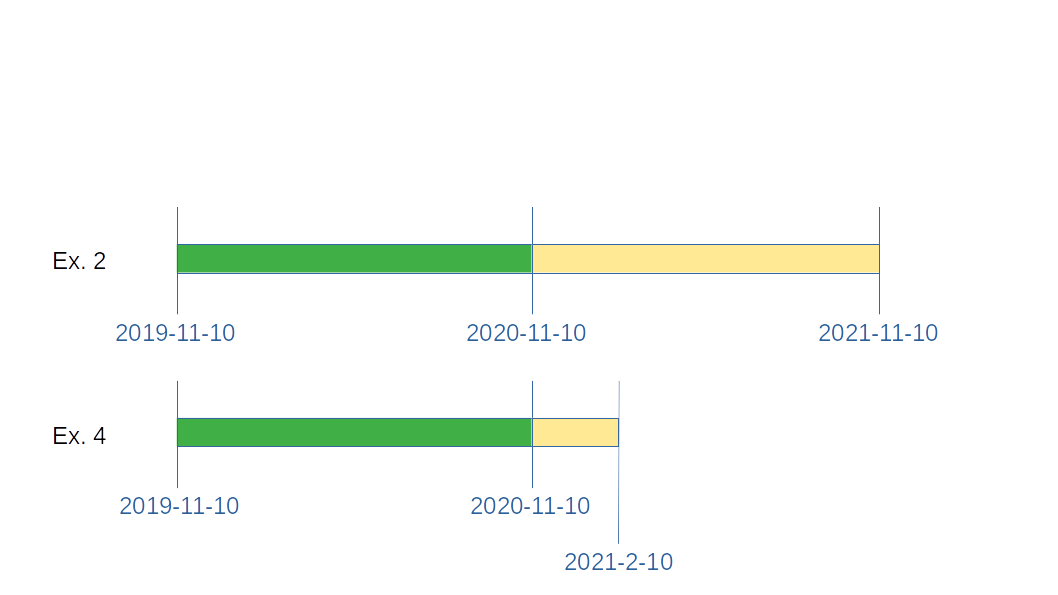
\includegraphics[width=0.8\linewidth]{time_flow.png}
%\end{figure}

%Here's some skeleton code to help you get started:
%
%\begin{Shaded}
%\begin{Highlighting}[]
%\ImportTok{from}\NormalTok{ dateutil }\ImportTok{import}\NormalTok{ relativedelta}
%
%\KeywordTok{def}\NormalTok{ generate_swap_dates(start_date, n_months):}
%\NormalTok{    dates }\OperatorTok{=}\NormalTok{ []}
%    \CommentTok{# your code here which adds all the relevant dates to the dates list}
%    \ControlFlowTok{return}\NormalTok{ dates}
%\end{Highlighting}
%\end{Shaded}
%
%\begin{Shaded}
%\begin{Highlighting}[]
%\CommentTok{# some tests to check if the function is working correctly}
%\ImportTok{from}\NormalTok{ datetime }\ImportTok{import}\NormalTok{ date}
%
%\ControlFlowTok{assert}\NormalTok{ generate_swap_dates(date(}\DecValTok{2019}\NormalTok{, }\DecValTok{11}\NormalTok{, }\DecValTok{10}\NormalTok{), }\DecValTok{12}\NormalTok{) }\OperatorTok{==}\NormalTok{ [date(}\DecValTok{2019}\NormalTok{, }\DecValTok{11}\NormalTok{, }\DecValTok{10}\NormalTok{), }
%\NormalTok{                                                       date(}\DecValTok{2020}\NormalTok{, }\DecValTok{11}\NormalTok{, }\DecValTok{10}\NormalTok{)]}
%\ControlFlowTok{assert}\NormalTok{ generate_swap_dates(date(}\DecValTok{2019}\NormalTok{, }\DecValTok{11}\NormalTok{, }\DecValTok{10}\NormalTok{), }\DecValTok{24}\NormalTok{) }\OperatorTok{==}\NormalTok{ [date(}\DecValTok{2019}\NormalTok{, }\DecValTok{11}\NormalTok{, }\DecValTok{10}\NormalTok{), }
%\NormalTok{                                                       date(}\DecValTok{2020}\NormalTok{, }\DecValTok{11}\NormalTok{, }\DecValTok{10}\NormalTok{), }
%\NormalTok{                                                       date(}\DecValTok{2021}\NormalTok{, }\DecValTok{11}\NormalTok{, }\DecValTok{10}\NormalTok{)]}
%
%\ControlFlowTok{assert}\NormalTok{ generate_swap_dates(date(}\DecValTok{2019}\NormalTok{, }\DecValTok{11}\NormalTok{, }\DecValTok{10}\NormalTok{), }\DecValTok{9}\NormalTok{) }\OperatorTok{==}\NormalTok{ [date(}\DecValTok{2019}\NormalTok{, }\DecValTok{11}\NormalTok{, }\DecValTok{10}\NormalTok{), }
%\NormalTok{                                                      date(}\DecValTok{2020}\NormalTok{, }\DecValTok{8}\NormalTok{, }\DecValTok{10}\NormalTok{)]}
%\ControlFlowTok{assert}\NormalTok{ generate_swap_dates(date(}\DecValTok{2019}\NormalTok{, }\DecValTok{11}\NormalTok{, }\DecValTok{10}\NormalTok{), }\DecValTok{15}\NormalTok{) }\OperatorTok{==}\NormalTok{ [date(}\DecValTok{2019}\NormalTok{, }\DecValTok{11}\NormalTok{, }\DecValTok{10}\NormalTok{), }
%\NormalTok{                                                       date(}\DecValTok{2020}\NormalTok{, }\DecValTok{11}\NormalTok{, }\DecValTok{10}\NormalTok{), }
%\NormalTok{                                                       date(}\DecValTok{2021}\NormalTok{, }\DecValTok{2}\NormalTok{, }\DecValTok{10}\NormalTok{)]}
%\end{Highlighting}
%\end{Shaded}
\end{Exercise}

\begin{Answer}
\begin{Verbatim}[commandchars=\\\{\}]
\PY{k+kn}{from} \PY{n+nn}{finmarkets} \PY{k}{import} \PY{n}{generate\PYZus{}swap\PYZus{}dates}
\PY{k+kn}{from} \PY{n+nn}{datetime} \PY{k}{import} \PY{n}{date}
\PY{k+kn}{from} \PY{n+nn}{dateutil}\PY{n+nn}{.}\PY{n+nn}{relativedelta} \PY{k}{import} \PY{n}{relativedelta}

\PY{k}{def} \PY{n+nf}{generate\PYZus{}swap\PYZus{}dates}\PY{p}{(}\PY{n}{start\PYZus{}date}\PY{p}{,} \PY{n}{n\PYZus{}months}\PY{p}{)}\PY{p}{:}
    \PY{n}{dates} \PY{o}{=} \PY{p}{[}\PY{p}{]}
    \PY{k}{for} \PY{n}{i} \PY{o+ow}{in} \PY{n+nb}{range}\PY{p}{(}\PY{l+m+mi}{0}\PY{p}{,} \PY{n}{n\PYZus{}months}\PY{p}{,} \PY{l+m+mi}{12}\PY{p}{)}\PY{p}{:}
        \PY{n}{dates}\PY{o}{.}\PY{n}{append}\PY{p}{(}\PY{n}{start\PYZus{}date} \PY{o}{+} \PY{n}{relativedelta}\PY{p}{(}\PY{n}{months}\PY{o}{=}\PY{n}{i}\PY{p}{)}\PY{p}{)}
    \PY{n}{dates}\PY{o}{.}\PY{n}{append}\PY{p}{(}\PY{n}{start\PYZus{}date} \PY{o}{+} \PY{n}{relativedelta}\PY{p}{(}\PY{n}{months}\PY{o}{=}\PY{n}{n\PYZus{}months}\PY{p}{)}\PY{p}{)}
    
    \PY{k}{return} \PY{n}{dates}


\PY{k}{assert} \PY{n}{generate\PYZus{}swap\PYZus{}dates}\PY{p}{(}\PY{n}{date}\PY{p}{(}\PY{l+m+mi}{2019}\PY{p}{,} \PY{l+m+mi}{11}\PY{p}{,} \PY{l+m+mi}{10}\PY{p}{)}\PY{p}{,} \PY{l+m+mi}{12}\PY{p}{)} \PY{o}{==} \PY{p}{[}\PY{n}{date}\PY{p}{(}\PY{l+m+mi}{2019}\PY{p}{,} \PY{l+m+mi}{11}\PY{p}{,} \PY{l+m+mi}{10}\PY{p}{)}\PY{p}{,} 
                                                       \PY{n}{date}\PY{p}{(}\PY{l+m+mi}{2020}\PY{p}{,} \PY{l+m+mi}{11}\PY{p}{,} \PY{l+m+mi}{10}\PY{p}{)}\PY{p}{]}
\PY{k}{assert} \PY{n}{generate\PYZus{}swap\PYZus{}dates}\PY{p}{(}\PY{n}{date}\PY{p}{(}\PY{l+m+mi}{2019}\PY{p}{,} \PY{l+m+mi}{11}\PY{p}{,} \PY{l+m+mi}{10}\PY{p}{)}\PY{p}{,} \PY{l+m+mi}{24}\PY{p}{)} \PY{o}{==} \PY{p}{[}\PY{n}{date}\PY{p}{(}\PY{l+m+mi}{2019}\PY{p}{,} \PY{l+m+mi}{11}\PY{p}{,} \PY{l+m+mi}{10}\PY{p}{)}\PY{p}{,} 
                                                       \PY{n}{date}\PY{p}{(}\PY{l+m+mi}{2020}\PY{p}{,} \PY{l+m+mi}{11}\PY{p}{,} \PY{l+m+mi}{10}\PY{p}{)}\PY{p}{,} 
                                                       \PY{n}{date}\PY{p}{(}\PY{l+m+mi}{2021}\PY{p}{,} \PY{l+m+mi}{11}\PY{p}{,} \PY{l+m+mi}{10}\PY{p}{)}\PY{p}{]}

\PY{k}{assert} \PY{n}{generate\PYZus{}swap\PYZus{}dates}\PY{p}{(}\PY{n}{date}\PY{p}{(}\PY{l+m+mi}{2019}\PY{p}{,} \PY{l+m+mi}{11}\PY{p}{,} \PY{l+m+mi}{10}\PY{p}{)}\PY{p}{,} \PY{l+m+mi}{9}\PY{p}{)} \PY{o}{==} \PY{p}{[}\PY{n}{date}\PY{p}{(}\PY{l+m+mi}{2019}\PY{p}{,} \PY{l+m+mi}{11}\PY{p}{,} \PY{l+m+mi}{10}\PY{p}{)}\PY{p}{,} 
                                                      \PY{n}{date}\PY{p}{(}\PY{l+m+mi}{2020}\PY{p}{,} \PY{l+m+mi}{8}\PY{p}{,} \PY{l+m+mi}{10}\PY{p}{)}\PY{p}{]}
\PY{k}{assert} \PY{n}{generate\PYZus{}swap\PYZus{}dates}\PY{p}{(}\PY{n}{date}\PY{p}{(}\PY{l+m+mi}{2019}\PY{p}{,} \PY{l+m+mi}{11}\PY{p}{,} \PY{l+m+mi}{10}\PY{p}{)}\PY{p}{,} \PY{l+m+mi}{15}\PY{p}{)} \PY{o}{==} \PY{p}{[}\PY{n}{date}\PY{p}{(}\PY{l+m+mi}{2019}\PY{p}{,} \PY{l+m+mi}{11}\PY{p}{,} \PY{l+m+mi}{10}\PY{p}{)}\PY{p}{,} 
                                                               \PY{n}{date}\PY{p}{(}\PY{l+m+mi}{2020}\PY{p}{,} \PY{l+m+mi}{11}\PY{p}{,} \PY{l+m+mi}{10}\PY{p}{)}\PY{p}{,} 
                                                               \PY{n}{date}\PY{p}{(}\PY{l+m+mi}{2021}\PY{p}{,} \PY{l+m+mi}{2}\PY{p}{,} \PY{l+m+mi}{10}\PY{p}{)}\PY{p}{]}
\end{Verbatim}
\end{Answer}

\clearpage
\chapter{Function and Classes}\label{introduction-to-python---lesson-4}

\section{Exercises}

\begin{Exercise}[label={ex:BS2}]
Take the code for the Black-Scholes formula from Exercise~\ref{ex:BS1} and wrap it in a function. Then, use this function to calculate the prices of calls with various strikes, using the following data.

\begin{Shaded}
\begin{Highlighting}[]
\NormalTok{s }\OperatorTok{=} \DecValTok{800}
\CommentTok{# strikes expressed as % of spot price}
\NormalTok{moneyness }\OperatorTok{=}\NormalTok{ [ }\FloatTok{0.5}\NormalTok{, }\FloatTok{0.75}\NormalTok{, }\FloatTok{0.825}\NormalTok{, }\FloatTok{1.0}\NormalTok{, }\FloatTok{1.125}\NormalTok{, }\FloatTok{1.25}\NormalTok{, }\FloatTok{1.5}\NormalTok{ ] }
\NormalTok{vol }\OperatorTok{=} \FloatTok{0.3}
\NormalTok{ttm }\OperatorTok{=} \FloatTok{0.75}
\NormalTok{r }\OperatorTok{=} \FloatTok{0.005}
\end{Highlighting}
\end{Shaded}

The output should be a dictionary mapping strikes to call prices.
\end{Exercise}

\begin{Answer}
\begin{tcolorbox}[size=fbox, boxrule=1pt, colback=cellbackground, colframe=cellborder]
\begin{Verbatim}[commandchars=\\\{\}]
\PY{k+kn}{from} \PY{n+nn}{math} \PY{k}{import} \PY{n}{log}\PY{p}{,} \PY{n}{exp}\PY{p}{,} \PY{n}{sqrt}
\PY{k+kn}{from} \PY{n+nn}{scipy}\PY{n+nn}{.}\PY{n+nn}{stats} \PY{k}{import} \PY{n}{norm}

\PY{k}{def} \PY{n+nf}{d1}\PY{p}{(}\PY{n}{S\PYZus{}t}\PY{p}{,} \PY{n}{K}\PY{p}{,} \PY{n}{r}\PY{p}{,} \PY{n}{vol}\PY{p}{,} \PY{n}{ttm}\PY{p}{)}\PY{p}{:}
    \PY{n}{num} \PY{o}{=} \PY{n}{log}\PY{p}{(}\PY{n}{S\PYZus{}t}\PY{o}{/}\PY{n}{K}\PY{p}{)} \PY{o}{+} \PY{p}{(}\PY{n}{r} \PY{o}{+} \PY{l+m+mf}{0.5}\PY{o}{*}\PY{n+nb}{pow}\PY{p}{(}\PY{n}{vol}\PY{p}{,} \PY{l+m+mi}{2}\PY{p}{)}\PY{p}{)} \PY{o}{*} \PY{n}{ttm}
    \PY{n}{den} \PY{o}{=} \PY{n}{vol} \PY{o}{*} \PY{n}{sqrt}\PY{p}{(}\PY{n}{ttm}\PY{p}{)}
    \PY{k}{return} \PY{n}{num}\PY{o}{/}\PY{n}{den}

\PY{k}{def} \PY{n+nf}{d2}\PY{p}{(}\PY{n}{S\PYZus{}t}\PY{p}{,} \PY{n}{K}\PY{p}{,} \PY{n}{r}\PY{p}{,} \PY{n}{vol}\PY{p}{,} \PY{n}{ttm}\PY{p}{)}\PY{p}{:}
    \PY{k}{return} \PY{n}{d1}\PY{p}{(}\PY{n}{S\PYZus{}t}\PY{p}{,} \PY{n}{K}\PY{p}{,} \PY{n}{r}\PY{p}{,} \PY{n}{vol}\PY{p}{,} \PY{n}{ttm}\PY{p}{)} \PY{o}{\PYZhy{}} \PY{n}{vol} \PY{o}{*} \PY{n}{sqrt}\PY{p}{(}\PY{n}{ttm}\PY{p}{)}

\PY{k}{def} \PY{n+nf}{call}\PY{p}{(}\PY{n}{S\PYZus{}t}\PY{p}{,} \PY{n}{K}\PY{p}{,} \PY{n}{r}\PY{p}{,} \PY{n}{vol}\PY{p}{,} \PY{n}{ttm}\PY{p}{)}\PY{p}{:}
    \PY{k}{return} \PY{n}{S\PYZus{}t} \PY{o}{*} \PY{n}{norm}\PY{o}{.}\PY{n}{cdf}\PY{p}{(}\PY{n}{d1}\PY{p}{(}\PY{n}{S\PYZus{}t}\PY{p}{,} \PY{n}{K}\PY{p}{,} \PY{n}{r}\PY{p}{,} \PY{n}{vol}\PY{p}{,} \PY{n}{ttm}\PY{p}{)}\PY{p}{)} \PYZbs{}
       \PY{o}{\PYZhy{}} \PY{n}{K} \PY{o}{*} \PY{n}{exp}\PY{p}{(}\PY{o}{\PYZhy{}}\PY{n}{r} \PY{o}{*} \PY{n}{ttm}\PY{p}{)} \PY{o}{*} \PY{n}{norm}\PY{o}{.}\PY{n}{cdf}\PY{p}{(}\PY{n}{d2}\PY{p}{(}\PY{n}{S\PYZus{}t}\PY{p}{,} \PY{n}{K}\PY{p}{,} \PY{n}{r}\PY{p}{,} \PY{n}{vol}\PY{p}{,} \PY{n}{ttm}\PY{p}{)}\PY{p}{)}

\PY{n}{s} \PY{o}{=} \PY{l+m+mi}{800}
\PY{c+c1}{\PYZsh{} strikes expressed as \PYZpc{} of spot price}
\PY{n}{moneyness} \PY{o}{=} \PY{p}{[} \PY{l+m+mf}{0.5}\PY{p}{,} \PY{l+m+mf}{0.75}\PY{p}{,} \PY{l+m+mf}{0.825}\PY{p}{,} \PYZbs{}
             \PY{l+m+mf}{1.0}\PY{p}{,} \PY{l+m+mf}{1.125}\PY{p}{,} \PY{l+m+mf}{1.25}\PY{p}{,} \PY{l+m+mf}{1.5} \PY{p}{]}
\PY{n}{vol} \PY{o}{=} \PY{l+m+mf}{0.3}
\PY{n}{ttm} \PY{o}{=} \PY{l+m+mf}{0.75}
\PY{n}{r} \PY{o}{=} \PY{l+m+mf}{0.005}

\PY{n}{result} \PY{o}{=} \PY{p}{\PYZob{}}\PY{p}{\PYZcb{}}
\PY{k}{for} \PY{n}{m} \PY{o+ow}{in} \PY{n}{moneyness}\PY{p}{:}
    \PY{n}{result}\PY{p}{[}\PY{n}{s}\PY{o}{*}\PY{n}{m}\PY{p}{]} \PY{o}{=} \PY{n}{call}\PY{p}{(}\PY{n}{s}\PY{p}{,} \PY{n}{m}\PY{o}{*}\PY{n}{s}\PY{p}{,} \PY{n}{r}\PY{p}{,} \PY{n}{vol}\PY{p}{,} \PY{n}{ttm}\PY{p}{)}
\PY{k}{print}\PY{p}{(}\PY{n}{result}\PY{p}{)}

\{400.0: 401.66074527896365,
  600.0: 213.9883852521275,
  660.0: 166.85957363897393,
  800.0: 84.03697017660357,
  900.0: 47.61880394696229,
  1000.0: 25.632722952585738,
  1200.0: 6.655275227771156\}
\end{Verbatim}
\end{tcolorbox}
\end{Answer}

\begin{Exercise}
Write two classes, \texttt{Circle} and \texttt{Rectangle} that given the radius and height, width respectively allow to compute area and perimeter of the two shapes. Test them with the following:

\begin{Shaded}
\begin{Highlighting}[]
\NormalTok{a_circle }\OperatorTok{=}\NormalTok{ Circle(}\DecValTok{5}\NormalTok{)}
\BuiltInTok{print}\NormalTok{ (}\StringTok{"My circle has an area of }\SpecialCharTok{\{\}}\StringTok{ m**2"}\NormalTok{.}\BuiltInTok{format}\NormalTok{(a_circle.area()))}

\NormalTok{a_rectangle }\OperatorTok{=}\NormalTok{ Rectangle(}\DecValTok{3}\NormalTok{, }\DecValTok{6}\NormalTok{)}
\BuiltInTok{print}\NormalTok{ (}\StringTok{"My rectangle has a perimeter of }\SpecialCharTok{\{\}}\StringTok{ m and an area of }\SpecialCharTok{\{\}}\StringTok{ m**2"}\NormalTok{ \textbackslash{}}
\NormalTok{    .}\BuiltInTok{format}\NormalTok{(a_rectangle.perimeter(), a_rectangle.area()))}
\end{Highlighting}
\end{Shaded}
\end{Exercise}

\begin{Answer}
\begin{tcolorbox}[size=fbox, boxrule=1pt, colback=cellbackground, colframe=cellborder]
\begin{Verbatim}[commandchars=\\\{\}]
\PY{k+kn}{from} \PY{n+nn}{math} \PY{k}{import} \PY{n}{pi}     
\PY{k}{class} \PY{n+nc}{Circle}\PY{p}{:}
    \PY{k}{def} \PY{n+nf}{\PYZus{}\PYZus{}init\PYZus{}\PYZus{}}\PY{p}{(}\PY{n+nb+bp}{self}\PY{p}{,} \PY{n}{radius}\PY{p}{)}\PY{p}{:}
        \PY{n+nb+bp}{self}\PY{o}{.}\PY{n}{radius} \PY{o}{=} \PY{n}{radius}

    \PY{k}{def} \PY{n+nf}{area}\PY{p}{(}\PY{n+nb+bp}{self}\PY{p}{)}\PY{p}{:}
        \PY{k}{return} \PY{n}{pi}\PY{o}{*}\PY{n+nb+bp}{self}\PY{o}{.}\PY{n}{radius}\PY{o}{*}\PY{o}{*}\PY{l+m+mi}{2}

\PY{k}{class} \PY{n+nc}{Rectangle}\PY{p}{:}
    \PY{k}{def} \PY{n+nf}{\PYZus{}\PYZus{}init\PYZus{}\PYZus{}}\PY{p}{(}\PY{n+nb+bp}{self}\PY{p}{,} \PY{n}{width}\PY{p}{,} \PY{n}{height}\PY{p}{)}\PY{p}{:}
        \PY{n+nb+bp}{self}\PY{o}{.}\PY{n}{height} \PY{o}{=} \PY{n}{height}
        \PY{n+nb+bp}{self}\PY{o}{.}\PY{n}{width} \PY{o}{=} \PY{n}{width}

    \PY{k}{def} \PY{n+nf}{area}\PY{p}{(}\PY{n+nb+bp}{self}\PY{p}{)}\PY{p}{:}
        \PY{k}{return} \PY{n+nb+bp}{self}\PY{o}{.}\PY{n}{width}\PY{o}{*}\PY{n+nb+bp}{self}\PY{o}{.}\PY{n}{height}

    \PY{k}{def} \PY{n+nf}{perimeter}\PY{p}{(}\PY{n+nb+bp}{self}\PY{p}{)}\PY{p}{:}
        \PY{k}{return} \PY{n+nb+bp}{self}\PY{o}{.}\PY{n}{width}\PY{o}{*}\PY{l+m+mi}{2} \PY{o}{+} \PY{n+nb+bp}{self}\PY{o}{.}\PY{n}{height}\PY{o}{*}\PY{l+m+mi}{2}

\PY{n}{circle} \PY{o}{=} \PY{n}{Circle}\PY{p}{(}\PY{l+m+mi}{5}\PY{p}{)}
\PY{n+nb}{print} \PY{p}{(}\PY{l+s+s2}{\PYZdq{}}\PY{l+s+s2}{My circle area is }\PY{l+s+si}{\PYZob{}:.1f\PYZcb{}}\PY{l+s+s2}{ m**2}\PY{l+s+s2}{\PYZdq{}}\PY{o}{.}\PY{n}{format}\PY{p}{(}\PY{n}{circle}\PY{o}{.}\PY{n}{area}\PY{p}{(}\PY{p}{)}\PY{p}{)}\PY{p}{)}

\PY{n}{rect} \PY{o}{=} \PY{n}{Rectangle}\PY{p}{(}\PY{l+m+mi}{3}\PY{p}{,} \PY{l+m+mi}{6}\PY{p}{)}
\PY{n+nb}{print} \PY{p}{(}\PY{l+s+s2}{\PYZdq{}}\PY{l+s+s2}{My rect area is }\PY{l+s+si}{\PYZob{}:.1f\PYZcb{}}\PY{l+s+s2}{ m**2 and the }\PY{l+s+s2}{\PYZdq{}}\PYZbs{}
       \PY{l+s+s2}{\PYZdq{}}\PY{l+s+s2}{perimeter is }\PY{l+s+si}{\PYZob{}\PYZcb{}}\PY{l+s+s2}{ m}\PY{l+s+s2}{\PYZdq{}}\PY{o}{.}\PY{n}{format}\PY{p}{(}\PY{n}{rect}\PY{o}{.}\PY{n}{area}\PY{p}{(}\PY{p}{)}\PY{p}{,} \PY{n}{rect}\PY{o}{.}\PY{n}{perimeter}\PY{p}{(}\PY{p}{)}\PY{p}{)}\PY{p}{)}

My circle area is 78.5 m**2
My rect area is 18.0 m**2 and the perimeter is 18 m
\end{Verbatim}
\end{tcolorbox}
\end{Answer}

\begin{Exercise}
Define a class \texttt{Songs}, its \texttt{\_\_init\_\_} should take as input a dictionary (\texttt{lyrics} that contains lyrics line by line). Define a method, \texttt{sing\_me\_a\_song} that prints each element of the lyrics in his own line. Also test it with the follwing input.

\begin{Shaded}
\begin{Highlighting}[]
\NormalTok{lyrics }\OperatorTok{=}\NormalTok{ \{}\StringTok{"Wonderwall"}\NormalTok{:[}\StringTok{"Today is gonna be the day"}\NormalTok{,}
                        \StringTok{"That they're gonna throw it back to you"}\NormalTok{,}
                        \StringTok{"By now you should've somehow"}\NormalTok{, }\StringTok{"..."}\NormalTok{], }
          \StringTok{"Wish you were here"}\NormalTok{:  [}\StringTok{"So, so you think you can tell"}\NormalTok{,}
                                  \StringTok{"Heaven from hell"}\NormalTok{,}
                                   \StringTok{"Blue skies from pain"}\NormalTok{, }\StringTok{"..."}\NormalTok{]\}}
\end{Highlighting}
\end{Shaded}
\end{Exercise}

\begin{Answer}
\begin{tcolorbox}[size=fbox, boxrule=1pt, colback=cellbackground, colframe=cellborder]
\begin{Verbatim}[commandchars=\\\{\}]
\PY{k}{class} \PY{n+nc}{Songs}\PY{p}{:}
        \PY{k}{def} \PY{n+nf}{\PYZus{}\PYZus{}init\PYZus{}\PYZus{}}\PY{p}{(}\PY{n+nb+bp}{self}\PY{p}{,} \PY{n}{lyrics}\PY{p}{)}\PY{p}{:}
            \PY{n+nb+bp}{self}\PY{o}{.}\PY{n}{lyrics} \PY{o}{=} \PY{n}{lyrics}
    
        \PY{k}{def} \PY{n+nf}{sing\PYZus{}me\PYZus{}a\PYZus{}song}\PY{p}{(}\PY{n+nb+bp}{self}\PY{p}{,} \PY{n}{title}\PY{p}{)}\PY{p}{:}
            \PY{n}{song} \PY{o}{=} \PY{n+nb+bp}{self}\PY{o}{.}\PY{n}{lyrics}\PY{p}{[}\PY{n}{title}\PY{p}{]}
            \PY{n+nb}{print} \PY{p}{(}\PY{l+s+s2}{\PYZdq{}}\PY{l+s+s2}{Title: }\PY{l+s+si}{\PYZob{}\PYZcb{}}\PY{l+s+s2}{\PYZdq{}}\PY{o}{.}\PY{n}{format}\PY{p}{(}\PY{n}{title}\PY{p}{)}\PY{p}{)}
            \PY{n+nb}{print} \PY{p}{(}\PY{l+s+s2}{\PYZdq{}}\PY{l+s+s2}{********************}\PY{l+s+s2}{\PYZdq{}}\PY{p}{)}
            \PY{k}{for} \PY{n}{line} \PY{o+ow}{in} \PY{n}{song}\PY{p}{:}
                \PY{n+nb}{print} \PY{p}{(}\PY{n}{line}\PY{p}{)}
    
\PY{n}{lyrics} \PY{o}{=} \PY{p}{\PYZob{}}\PY{l+s+s2}{\PYZdq{}}\PY{l+s+s2}{Wonderwall}\PY{l+s+s2}{\PYZdq{}}\PY{p}{:}\PY{p}{[}\PY{l+s+s2}{\PYZdq{}}\PY{l+s+s2}{Today is gonna be the day}\PY{l+s+s2}{\PYZdq{}}\PY{p}{,}
                        \PY{l+s+s2}{\PYZdq{}}\PY{l+s+s2}{That they}\PY{l+s+s2}{\PYZsq{}}\PY{l+s+s2}{re gonna throw it back to you}\PY{l+s+s2}{\PYZdq{}}\PY{p}{,}
                        \PY{l+s+s2}{\PYZdq{}}\PY{l+s+s2}{By now you should}\PY{l+s+s2}{\PYZsq{}}\PY{l+s+s2}{ve somehow}\PY{l+s+s2}{\PYZdq{}}\PY{p}{,} \PY{l+s+s2}{\PYZdq{}}\PY{l+s+s2}{...}\PY{l+s+s2}{\PYZdq{}}\PY{p}{]}\PY{p}{,} 
          \PY{l+s+s2}{\PYZdq{}}\PY{l+s+s2}{Vado al massimo}\PY{l+s+s2}{\PYZdq{}}\PY{p}{:}  \PY{p}{[}\PY{l+s+s2}{\PYZdq{}}\PY{l+s+s2}{Voglio veder come va a finire}\PY{l+s+s2}{\PYZdq{}}\PY{p}{,}
                        \PY{l+s+s2}{\PYZdq{}}\PY{l+s+s2}{Andando al massimo senza frenare}\PY{l+s+s2}{\PYZdq{}}
                        \PY{l+s+s2}{\PYZdq{}}\PY{l+s+s2}{Voglio vedere se davvero poi}\PY{l+s+s2}{\PYZdq{}}\PY{p}{,}
                        \PY{l+s+s2}{\PYZdq{}}\PY{l+s+s2}{Si va a finir male}\PY{l+s+s2}{\PYZdq{}}\PY{p}{,} \PY{l+s+s2}{\PYZdq{}}\PY{l+s+s2}{...}\PY{l+s+s2}{\PYZdq{}}\PY{p}{]}\PY{p}{\PYZcb{}}

\PY{n}{songs} \PY{o}{=} \PY{n}{Songs}\PY{p}{(}\PY{n}{lyrics}\PY{p}{)}
\PY{n}{songs}\PY{o}{.}\PY{n}{sing\PYZus{}me\PYZus{}a\PYZus{}song}\PY{p}{(}\PY{l+s+s2}{\PYZdq{}}\PY{l+s+s2}{Wonderwall}\PY{l+s+s2}{\PYZdq{}}\PY{p}{)}

Title: Wonderwall
********************
Today is gonna be the day
That they're gonna throw it back to you
By now you should've somehow
{\ldots}
\end{Verbatim}
\end{tcolorbox}
\end{Answer}

\begin{Exercise}
Define a Point2D class that represent a point in a plane. Its \texttt{\_\_init\_\_} method should accept the point coordinates \texttt{x} and \texttt{y}. Write a method \texttt{distanceTo} that compute the distance of the point to another passed as input. Test the class by printing the distance of the point \(P=(4, 5)\) to the origin \(P=(0,0)\) and to \(P=(3,4)\). \\
\textbf{Hint:} in the Cartesian plane the distance between two points is: $\sqrt{(x_1 - x_2)^2 + (y_1 - y_2)^2}$.
\end{Exercise}

\begin{Answer}
\begin{tcolorbox}[size=fbox, boxrule=1pt, colback=cellbackground, colframe=cellborder]
\begin{Verbatim}[commandchars=\\\{\}]
\PY{k+kn}{from} \PY{n+nn}{math} \PY{k}{import} \PY{n}{sqrt}
\PY{k}{class} \PY{n+nc}{Point2D}\PY{p}{:}
    \PY{k}{def} \PY{n+nf}{\PYZus{}\PYZus{}init\PYZus{}\PYZus{}}\PY{p}{(}\PY{n+nb+bp}{self}\PY{p}{,} \PY{n}{x}\PY{p}{,} \PY{n}{y}\PY{p}{)}\PY{p}{:}
        \PY{n+nb+bp}{self}\PY{o}{.}\PY{n}{x} \PY{o}{=} \PY{n}{x}
        \PY{n+nb+bp}{self}\PY{o}{.}\PY{n}{y} \PY{o}{=} \PY{n}{y}

    \PY{k}{def} \PY{n+nf}{distanceTo}\PY{p}{(}\PY{n+nb+bp}{self}\PY{p}{,} \PY{n}{x}\PY{p}{,} \PY{n}{y}\PY{p}{)}\PY{p}{:}
        \PY{n}{dist} \PY{o}{=} \PY{n}{sqrt}\PY{p}{(}\PY{p}{(}\PY{n+nb+bp}{self}\PY{o}{.}\PY{n}{x}\PY{o}{\PYZhy{}}\PY{n}{x}\PY{p}{)}\PY{o}{*}\PY{o}{*}\PY{l+m+mi}{2} \PY{o}{+} \PY{p}{(}\PY{n+nb+bp}{self}\PY{o}{.}\PY{n}{y} \PY{o}{\PYZhy{}} \PY{n}{y}\PY{p}{)}\PY{o}{*}\PY{o}{*}\PY{l+m+mi}{2}\PY{p}{)}
        \PY{k}{return} \PY{n}{dist}

    \PY{k}{def} \PY{n+nf}{distanceTo\PYZus{}v2}\PY{p}{(}\PY{n+nb+bp}{self}\PY{p}{,} \PY{n}{p}\PY{p}{)}\PY{p}{:}
        \PY{n}{dist} \PY{o}{=} \PY{n}{sqrt}\PY{p}{(}\PY{p}{(}\PY{n+nb+bp}{self}\PY{o}{.}\PY{n}{x}\PY{o}{\PYZhy{}}\PY{n}{p}\PY{p}{[}\PY{l+m+mi}{0}\PY{p}{]}\PY{p}{)}\PY{o}{*}\PY{o}{*}\PY{l+m+mi}{2} \PY{o}{+} \PY{p}{(}\PY{n+nb+bp}{self}\PY{o}{.}\PY{n}{y} \PY{o}{\PYZhy{}} \PY{n}{p}\PY{p}{[}\PY{l+m+mi}{1}\PY{p}{]}\PY{p}{)}\PY{o}{*}\PY{o}{*}\PY{l+m+mi}{2}\PY{p}{)}
        \PY{k}{return} \PY{n}{dist}

    \PY{k}{def} \PY{n+nf}{distanceTo\PYZus{}v3}\PY{p}{(}\PY{n+nb+bp}{self}\PY{p}{,} \PY{n}{p}\PY{p}{)}\PY{p}{:}
        \PY{n}{dist} \PY{o}{=} \PY{n}{sqrt}\PY{p}{(}\PY{p}{(}\PY{n+nb+bp}{self}\PY{o}{.}\PY{n}{x}\PY{o}{\PYZhy{}}\PY{n}{p}\PY{o}{.}\PY{n}{x}\PY{p}{)}\PY{o}{*}\PY{o}{*}\PY{l+m+mi}{2} \PY{o}{+} \PY{p}{(}\PY{n+nb+bp}{self}\PY{o}{.}\PY{n}{y} \PY{o}{\PYZhy{}} \PY{n}{p}\PY{o}{.}\PY{n}{y}\PY{p}{)}\PY{o}{*}\PY{o}{*}\PY{l+m+mi}{2}\PY{p}{)}
        \PY{k}{return} \PY{n}{dist}

\PY{n}{point} \PY{o}{=} \PY{n}{Point2D}\PY{p}{(}\PY{l+m+mi}{4}\PY{p}{,} \PY{l+m+mi}{5}\PY{p}{)}
\PY{n}{p0} \PY{o}{=} \PY{p}{(}\PY{l+m+mi}{0}\PY{p}{,} \PY{l+m+mi}{0}\PY{p}{)}
\PY{n}{point0} \PY{o}{=} \PY{n}{Point2D}\PY{p}{(}\PY{l+m+mi}{0}\PY{p}{,} \PY{l+m+mi}{0}\PY{p}{)}
\PY{n+nb}{print} \PY{p}{(}\PY{l+s+s2}{\PYZdq{}}\PY{l+s+s2}{distance to p0: }\PY{l+s+si}{\PYZob{}:.2f\PYZcb{}}\PY{l+s+s2}{\PYZdq{}}\PY{o}{.}\PY{n}{format}\PY{p}{(}\PY{n}{point}\PY{o}{.}\PY{n}{distanceTo}\PY{p}{(}\PY{n}{p0}\PY{p}{[}\PY{l+m+mi}{0}\PY{p}{]}\PY{p}{,} \PY{n}{p0}\PY{p}{[}\PY{l+m+mi}{1}\PY{p}{]}\PY{p}{)}\PY{p}{)}\PY{p}{)}
\PY{n+nb}{print} \PY{p}{(}\PY{l+s+s2}{\PYZdq{}}\PY{l+s+s2}{distance\PYZus{}v2 to p0: }\PY{l+s+si}{\PYZob{}:.2f\PYZcb{}}\PY{l+s+s2}{\PYZdq{}}\PY{o}{.}\PY{n}{format}\PY{p}{(}\PY{n}{point}\PY{o}{.}\PY{n}{distanceTo\PYZus{}v2}\PY{p}{(}\PY{n}{p0}\PY{p}{)}\PY{p}{)}\PY{p}{)}
\PY{n+nb}{print} \PY{p}{(}\PY{l+s+s2}{\PYZdq{}}\PY{l+s+s2}{distance\PYZus{}v3 to p0: }\PY{l+s+si}{\PYZob{}:.2f\PYZcb{}}\PY{l+s+s2}{\PYZdq{}}\PY{o}{.}\PY{n}{format}\PY{p}{(}\PY{n}{point}\PY{o}{.}\PY{n}{distanceTo\PYZus{}v3}\PY{p}{(}\PY{n}{point0}\PY{p}{)}\PY{p}{)}\PY{p}{)}

\PY{n}{p1} \PY{o}{=} \PY{p}{(}\PY{l+m+mi}{3}\PY{p}{,} \PY{l+m+mi}{4}\PY{p}{)}
\PY{n}{point1} \PY{o}{=} \PY{n}{Point2D}\PY{p}{(}\PY{l+m+mi}{3}\PY{p}{,} \PY{l+m+mi}{4}\PY{p}{)}
\PY{n+nb}{print} \PY{p}{(}\PY{l+s+s2}{\PYZdq{}}\PY{l+s+s2}{distance to p1: }\PY{l+s+si}{\PYZob{}:.2f\PYZcb{}}\PY{l+s+s2}{\PYZdq{}}\PY{o}{.}\PY{n}{format}\PY{p}{(}\PY{n}{point}\PY{o}{.}\PY{n}{distanceTo}\PY{p}{(}\PY{n}{p1}\PY{p}{[}\PY{l+m+mi}{0}\PY{p}{]}\PY{p}{,} \PY{n}{p1}\PY{p}{[}\PY{l+m+mi}{1}\PY{p}{]}\PY{p}{)}\PY{p}{)}\PY{p}{)}
\PY{n+nb}{print} \PY{p}{(}\PY{l+s+s2}{\PYZdq{}}\PY{l+s+s2}{distance\PYZus{}v2 to p1: }\PY{l+s+si}{\PYZob{}:.2f\PYZcb{}}\PY{l+s+s2}{\PYZdq{}}\PY{o}{.}\PY{n}{format}\PY{p}{(}\PY{n}{point}\PY{o}{.}\PY{n}{distanceTo\PYZus{}v2}\PY{p}{(}\PY{n}{p1}\PY{p}{)}\PY{p}{)}\PY{p}{)}
\PY{n+nb}{print} \PY{p}{(}\PY{l+s+s2}{\PYZdq{}}\PY{l+s+s2}{distance\PYZus{}v3 to p1: }\PY{l+s+si}{\PYZob{}:.2f\PYZcb{}}\PY{l+s+s2}{\PYZdq{}}\PY{o}{.}\PY{n}{format}\PY{p}{(}\PY{n}{point}\PY{o}{.}\PY{n}{distanceTo\PYZus{}v3}\PY{p}{(}\PY{n}{point1}\PY{p}{)}\PY{p}{)}\PY{p}{)}

distance to p0: 6.40
distance\_v2 to p0: 6.40
distance\_v3 to p0: 6.40
distance to p1: 1.41
distance\_v2 to p1: 1.41
distance\_v3 to p1: 1.41
\end{Verbatim}
\end{tcolorbox}
\end{Answer}

\clearpage
\chapter{Data Manipulation and Its Representation}\label{introduction-to-python---lesson-5}

\begin{Exercise}
Using \texttt{pandas} import data stored in \href{https://drive.google.com/file/d/1Uu9lQorvzM-1xwRKPNszaSqlCYAiY-gr/view?usp=sharing}{\texttt{stock\_market.xlsx}} (click on the name to see and download it). With the resulting dataframe determine:
\Question remove duplicates and missing data (how many rows are left ?)
\Question stocks with positive variation;
\Question the first five stocks with the lowest price.
\end{Exercise}
\clearpage
\begin{Answer}
  \Question
First load the excel file into a dataframe and look at data structure.

\begin{codebox}[size=fbox, boxrule=1pt, colback=cellbackground, colframe=cellborder]
\begin{Verbatim}[commandchars=\\\{\}]
\PY{k+kn}{import} \PY{n+nn}{pandas} \PY{k}{as} \PY{n+nn}{pd}

\PY{n}{df} \PY{o}{=} \PY{n}{pd}\PY{o}{.}\PY{n}{read\PYZus{}excel}\PY{p}{(}\PY{l+s+s2}{\PYZdq{}}\PY{l+s+s2}{stock\PYZus{}market.xlsx}\PY{l+s+s2}{\PYZdq{}}\PY{p}{)}

\PY{n+nb}{print} \PY{p}{(}\PY{n+nb}{len}\PY{p}{(}\PY{n}{df}\PY{p}{)}\PY{p}{)}
\PY{n}{df}\PY{o}{.}\PY{n}{head}\PY{p}{(}\PY{p}{)}

51

  Symbol                      Name   Price  Change  Change\%  Volume (M)  \textbackslash{}
0     GE  General Electric Company    6.07   -0.19  -0.0304     142.732
1    NOK         Nokia Corporation    4.78    0.33   0.0742     117.960
2      F        Ford Motor Company    6.61   -0.13  -0.0193     115.394
3   PINS           Pinterest, Inc.   34.29    9.10   0.3613     111.864
4   AAPL                Apple Inc.  425.04   40.28   0.1047      93.574

   Avg Volume (M)  Market Cap (B)
0         102.268          53.132
1          31.296          27.083
2          87.719          26.288
3          15.550          20.110
4          35.035        1821.000
\end{Verbatim}
\end{codebox}
        
As usual if we are not sure that our data is \emph{clean} we should check for duplicates and NaN and take care of them. The \texttt{duplicated} method returns the status of each row (duplicate or not, True or False). If we would like just to see the duplicated entries we could combine the \texttt{duplicated} method with the selection syntax like this:

\begin{codebox}[size=fbox, boxrule=1pt, colback=cellbackground, colframe=cellborder]
\begin{Verbatim}[commandchars=\\\{\}]
\PY{n}{df}\PY{p}{[}\PY{n}{df}\PY{o}{.}\PY{n}{duplicated}\PY{p}{(}\PY{p}{)} \PY{o}{==} \PY{k+kc}{True}\PY{p}{]}

   Symbol         Name  Price  Change  Change\%  Volume (M)  Avg Volume (M)  \textbackslash{}
40    RUN  Sunrun Inc.  36.69    0.02   0.0005      20.113           3.604

    Market Cap (B)
40           4.489
\end{Verbatim}
\end{codebox}
        
So it looks like we have just one duplicate and we can remove it:

\begin{codebox}[size=fbox, boxrule=1pt, colback=cellbackground, colframe=cellborder]
\begin{Verbatim}[commandchars=\\\{\}]
\PY{n+nb}{print} \PY{p}{(}\PY{l+s+s2}{\PYZdq{}}\PY{l+s+s2}{Before duplicates removal: }\PY{l+s+si}{\PYZob{}\PYZcb{}}\PY{l+s+s2}{\PYZdq{}}\PY{o}{.}\PY{n}{format}\PY{p}{(}\PY{n+nb}{len}\PY{p}{(}\PY{n}{df}\PY{p}{)}\PY{p}{)}\PY{p}{)}
\PY{n}{df} \PY{o}{=} \PY{n}{df}\PY{o}{.}\PY{n}{drop\PYZus{}duplicates}\PY{p}{(}\PY{p}{)}
\PY{n+nb}{print} \PY{p}{(}\PY{l+s+s2}{\PYZdq{}}\PY{l+s+s2}{After duplicates removal: }\PY{l+s+si}{\PYZob{}\PYZcb{}}\PY{l+s+s2}{\PYZdq{}}\PY{o}{.}\PY{n}{format}\PY{p}{(}\PY{n+nb}{len}\PY{p}{(}\PY{n}{df}\PY{p}{)}\PY{p}{)}\PY{p}{)}

Before duplicates removal: 50
After duplicates removal: 50
\end{Verbatim}
\end{codebox}

Then we need to take care of the NaN, again if we want to check the rows with NaN we can select (here the syntax is a little bit more complicated since we need to use \texttt{any} to look for Nan in every column):

\begin{codebox}[size=fbox, boxrule=1pt, colback=cellbackground, colframe=cellborder]
\begin{Verbatim}[commandchars=\\\{\}]
\PY{n}{df}\PY{p}{[}\PY{n}{df}\PY{o}{.}\PY{n}{isna}\PY{p}{(}\PY{p}{)}\PY{o}{.}\PY{n}{any}\PY{p}{(}\PY{n}{axis}\PY{o}{=}\PY{l+m+mi}{1}\PY{p}{)}\PY{p}{]}

   Symbol                                 Name  Price  Change  Change\%  \textbackslash{}
23   NCLH  Norwegian Cruise Line Holdings Ltd.  13.64   -0.53  -0.0374
47    NBL                   Noble Energy, Inc.    NaN   -0.23  -0.0225

    Volume (M)  Avg Volume (M)  Market Cap (B)
23      28.402          64.895             NaN
47      18.462          13.535           4.795
\end{Verbatim}
\end{codebox}
        
Since we don't want to artificially modify our sample we just drop rows with NaN:

\begin{codebox}[size=fbox, boxrule=1pt, colback=cellbackground, colframe=cellborder]
\begin{Verbatim}[commandchars=\\\{\}]
\PY{n+nb}{print} \PY{p}{(}\PY{l+s+s2}{\PYZdq{}}\PY{l+s+s2}{Before NaN removal: }\PY{l+s+si}{\PYZob{}\PYZcb{}}\PY{l+s+s2}{\PYZdq{}}\PY{o}{.}\PY{n}{format}\PY{p}{(}\PY{n+nb}{len}\PY{p}{(}\PY{n}{df}\PY{p}{)}\PY{p}{)}\PY{p}{)}
\PY{n}{df} \PY{o}{=} \PY{n}{df}\PY{o}{.}\PY{n}{dropna}\PY{p}{(}\PY{p}{)}
\PY{n+nb}{print} \PY{p}{(}\PY{l+s+s2}{\PYZdq{}}\PY{l+s+s2}{After NaN removal: }\PY{l+s+si}{\PYZob{}\PYZcb{}}\PY{l+s+s2}{\PYZdq{}}\PY{o}{.}\PY{n}{format}\PY{p}{(}\PY{n+nb}{len}\PY{p}{(}\PY{n}{df}\PY{p}{)}\PY{p}{)}\PY{p}{)}

Before NaN removal: 51
After NaN removal: 49
\end{Verbatim}
\end{codebox}

\Question
The second point asks to determine the companies with a daily positive variation. Clearly we have to apply to the dataframe a selection on the ``Change'' (or ``Change\%'') column requiring positive values.

\begin{codebox}[size=fbox, boxrule=1pt, colback=cellbackground, colframe=cellborder]
\begin{Verbatim}[commandchars=\\\{\}]
\PY{n}{pos\PYZus{}var} \PY{o}{=} \PY{n}{df}\PY{p}{[}\PY{n}{df}\PY{o}{.}\PY{n}{loc}\PY{p}{[}\PY{p}{:}\PY{p}{,} \PY{l+s+s2}{\PYZdq{}}\PY{l+s+s2}{Change}\PY{l+s+s2}{\PYZdq{}}\PY{p}{]} \PY{o}{\PYZgt{}} \PY{l+m+mi}{0}\PY{p}{]}

\PY{n+nb}{print} \PY{p}{(}\PY{n+nb}{len}\PY{p}{(}\PY{n}{pos\PYZus{}var}\PY{p}{)}\PY{p}{)}
\PY{n}{pos\PYZus{}var}\PY{o}{.}\PY{n}{head}\PY{p}{(}\PY{p}{)} \PY{c+c1}{\PYZsh{} just printing the first 5 rows}

16

  Symbol                         Name   Price  Change  Change\%  Volume (M)  \textbackslash{}
1    NOK            Nokia Corporation    4.78    0.33   0.0742     117.960
3   PINS              Pinterest, Inc.   34.29    9.10   0.3613     111.864
4   AAPL                   Apple Inc.  425.04   40.28   0.1047      93.574
6    BAC  Bank of America Corporation   24.88    0.04   0.0016      62.039
8     FB               Facebook, Inc.  253.67   19.17   0.0817      53.030

   Avg Volume (M)  Market Cap (B)
1          31.296          27.083
3          15.550          20.110
4          35.035        1821.000
6          72.793         215.562
8          24.521         723.726
\end{Verbatim}
\end{codebox}
        
So in origin we had 48 stocks and just 16 have a positive variation of its price.

\Question
The last question requires to print the first 5 stocks with the lowest prices. In this case it is enough to sort by price the dataframe (ascending) and then just select the first 5 entries.

\begin{codebox}[size=fbox, boxrule=1pt, colback=cellbackground, colframe=cellborder]
\begin{Verbatim}[commandchars=\\\{\}]
\PY{n}{highest\PYZus{}price} \PY{o}{=} \PY{n}{df}\PY{o}{.}\PY{n}{sort\PYZus{}values}\PY{p}{(}\PY{n}{by}\PY{o}{=}\PY{p}{[}\PY{l+s+s1}{\PYZsq{}}\PY{l+s+s1}{Price}\PY{l+s+s1}{\PYZsq{}}\PY{p}{]}\PY{p}{,} \PY{n}{ascending}\PY{o}{=}\PY{k+kc}{True}\PY{p}{)}\PY{p}{[}\PY{p}{:}\PY{l+m+mi}{5}\PY{p}{]}

\PY{n}{highest\PYZus{}price}

   Symbol                      Name  Price  Change  Change\%  Volume (M)  \textbackslash{}
25   ABEV               Ambev S. A.   2.68   -0.16  -0.0563      26.136
32    BBD      Banco Bradesco S. A.   4.22   -0.32  -0.0705      22.129
1     NOK         Nokia Corporation   4.78    0.33   0.0742     117.960
15    OPK         OPKO Health, Inc.   5.15   -0.76  -0.1286      35.762
33    MRO  Marathon Oil Corporation   5.49   -0.02  -0.0036      21.249

    Avg Volume (M)  Market Cap (B)
25          36.654          41.999
32          22.046          36.739
1           31.296          27.083
15          17.792           3.450
33          34.098           4.339
\end{Verbatim}
\end{codebox}
\end{Answer}

\begin{Exercise}
Given the following discount factors plot the resulting discount curve,
possibly adding axis labels and legend.

\begin{Shaded}
\begin{Highlighting}[]
\NormalTok{dfs }\OperatorTok{=}\NormalTok{ [}\FloatTok{1.0}\NormalTok{, }\FloatTok{1.0014907894567657}\NormalTok{, }\FloatTok{1.0031038833235129}\NormalTok{, }\FloatTok{1.0047764800189012}\NormalTok{,}
       \FloatTok{1.0065986105304596}\NormalTok{, }\FloatTok{1.014496095021891}\NormalTok{, }\FloatTok{1.022687560553011}\NormalTok{,}
       \FloatTok{1.0303585751965112}\NormalTok{, }\FloatTok{1.0369440287181253}\NormalTok{, }\FloatTok{1.0422287558021188}\NormalTok{,}
       \FloatTok{1.0461834022163963}\NormalTok{, }\FloatTok{1.0489228953047331}\NormalTok{, }\FloatTok{1.0505725627906783}\NormalTok{,}
       \FloatTok{1.0513323539753632}\NormalTok{, }\FloatTok{1.0513777790851995}\NormalTok{, }\FloatTok{1.0508768750534248}\NormalTok{,}
       \FloatTok{1.049935905228433}\NormalTok{, }\FloatTok{1.0486741093761602}\NormalTok{, }\FloatTok{1.047175413484517}\NormalTok{,}
       \FloatTok{1.0455115431993336}\NormalTok{, }\FloatTok{1.0437147446170034}\NormalTok{, }\FloatTok{1.0418294960952215}\NormalTok{,}
       \FloatTok{1.0398823957504923}\NormalTok{, }\FloatTok{1.0378979499878478}\NormalTok{, }\FloatTok{1.0358789099539805}\NormalTok{,}
       \FloatTok{1.0338409767365169}\NormalTok{, }\FloatTok{1.031791178324756}\NormalTok{, }\FloatTok{1.0297378455884902}\NormalTok{,}
       \FloatTok{1.0276772747965244}\NormalTok{, }\FloatTok{1.0256154380560942}\NormalTok{, }\FloatTok{1.0235543974485939}\NormalTok{,}
       \FloatTok{1.0214974135391857}\NormalTok{, }\FloatTok{1.0194401540150835}\NormalTok{, }\FloatTok{1.0173862951028778}\NormalTok{]}

\NormalTok{pillars }\OperatorTok{=}\NormalTok{ [datetime.date(}\DecValTok{2020}\NormalTok{, }\DecValTok{8}\NormalTok{, }\DecValTok{3}\NormalTok{), datetime.date(}\DecValTok{2020}\NormalTok{, }\DecValTok{11}\NormalTok{, }\DecValTok{3}\NormalTok{), }
\NormalTok{           datetime.date(}\DecValTok{2021}\NormalTok{, }\DecValTok{2}\NormalTok{, }\DecValTok{3}\NormalTok{), datetime.date(}\DecValTok{2021}\NormalTok{, }\DecValTok{5}\NormalTok{, }\DecValTok{3}\NormalTok{), }
\NormalTok{           datetime.date(}\DecValTok{2021}\NormalTok{, }\DecValTok{8}\NormalTok{, }\DecValTok{3}\NormalTok{), datetime.date(}\DecValTok{2022}\NormalTok{, }\DecValTok{8}\NormalTok{, }\DecValTok{3}\NormalTok{),}
\NormalTok{           datetime.date(}\DecValTok{2023}\NormalTok{, }\DecValTok{8}\NormalTok{, }\DecValTok{3}\NormalTok{), datetime.date(}\DecValTok{2024}\NormalTok{, }\DecValTok{8}\NormalTok{, }\DecValTok{3}\NormalTok{), }
\NormalTok{           datetime.date(}\DecValTok{2025}\NormalTok{, }\DecValTok{8}\NormalTok{, }\DecValTok{3}\NormalTok{), datetime.date(}\DecValTok{2026}\NormalTok{, }\DecValTok{8}\NormalTok{, }\DecValTok{3}\NormalTok{), }
\NormalTok{           datetime.date(}\DecValTok{2027}\NormalTok{, }\DecValTok{8}\NormalTok{, }\DecValTok{3}\NormalTok{), datetime.date(}\DecValTok{2028}\NormalTok{, }\DecValTok{8}\NormalTok{, }\DecValTok{3}\NormalTok{),}
\NormalTok{           datetime.date(}\DecValTok{2029}\NormalTok{, }\DecValTok{8}\NormalTok{, }\DecValTok{3}\NormalTok{), datetime.date(}\DecValTok{2030}\NormalTok{, }\DecValTok{8}\NormalTok{, }\DecValTok{3}\NormalTok{), }
\NormalTok{           datetime.date(}\DecValTok{2031}\NormalTok{, }\DecValTok{8}\NormalTok{, }\DecValTok{3}\NormalTok{), datetime.date(}\DecValTok{2032}\NormalTok{, }\DecValTok{8}\NormalTok{, }\DecValTok{3}\NormalTok{), }
\NormalTok{           datetime.date(}\DecValTok{2033}\NormalTok{, }\DecValTok{8}\NormalTok{, }\DecValTok{3}\NormalTok{), datetime.date(}\DecValTok{2034}\NormalTok{, }\DecValTok{8}\NormalTok{, }\DecValTok{3}\NormalTok{),}
\NormalTok{           datetime.date(}\DecValTok{2035}\NormalTok{, }\DecValTok{8}\NormalTok{, }\DecValTok{3}\NormalTok{), datetime.date(}\DecValTok{2036}\NormalTok{, }\DecValTok{8}\NormalTok{, }\DecValTok{3}\NormalTok{), }
\NormalTok{           datetime.date(}\DecValTok{2037}\NormalTok{, }\DecValTok{8}\NormalTok{, }\DecValTok{3}\NormalTok{), datetime.date(}\DecValTok{2038}\NormalTok{, }\DecValTok{8}\NormalTok{, }\DecValTok{3}\NormalTok{), }
\NormalTok{           datetime.date(}\DecValTok{2039}\NormalTok{, }\DecValTok{8}\NormalTok{, }\DecValTok{3}\NormalTok{), datetime.date(}\DecValTok{2040}\NormalTok{, }\DecValTok{8}\NormalTok{, }\DecValTok{3}\NormalTok{),}
\NormalTok{           datetime.date(}\DecValTok{2041}\NormalTok{, }\DecValTok{8}\NormalTok{, }\DecValTok{3}\NormalTok{), datetime.date(}\DecValTok{2042}\NormalTok{, }\DecValTok{8}\NormalTok{, }\DecValTok{3}\NormalTok{), }
\NormalTok{           datetime.date(}\DecValTok{2043}\NormalTok{, }\DecValTok{8}\NormalTok{, }\DecValTok{3}\NormalTok{), datetime.date(}\DecValTok{2044}\NormalTok{, }\DecValTok{8}\NormalTok{, }\DecValTok{3}\NormalTok{), }
\NormalTok{           datetime.date(}\DecValTok{2045}\NormalTok{, }\DecValTok{8}\NormalTok{, }\DecValTok{3}\NormalTok{), datetime.date(}\DecValTok{2046}\NormalTok{, }\DecValTok{8}\NormalTok{, }\DecValTok{3}\NormalTok{),}
\NormalTok{           datetime.date(}\DecValTok{2047}\NormalTok{, }\DecValTok{8}\NormalTok{, }\DecValTok{3}\NormalTok{), datetime.date(}\DecValTok{2048}\NormalTok{, }\DecValTok{8}\NormalTok{, }\DecValTok{3}\NormalTok{), }
\NormalTok{           datetime.date(}\DecValTok{2049}\NormalTok{, }\DecValTok{8}\NormalTok{, }\DecValTok{3}\NormalTok{), datetime.date(}\DecValTok{2050}\NormalTok{, }\DecValTok{8}\NormalTok{, }\DecValTok{3}\NormalTok{)]}
\end{Highlighting}
\end{Shaded}
\end{Exercise}

\begin{Answer}
\begin{codebox}[size=fbox, boxrule=1pt, colback=cellbackground, colframe=cellborder]
\begin{Verbatim}[commandchars=\\\{\}]
\PY{k+kn}{import} \PY{n+nn}{datetime}

\PY{n}{dfs} \PY{o}{=} \PY{p}{[}\PY{l+m+mf}{1.0}\PY{p}{,} \PY{l+m+mf}{1.0014907894567657}\PY{p}{,} \PY{l+m+mf}{1.0031038833235129}\PY{p}{,} \PY{l+m+mf}{1.0047764800189012}\PY{p}{, ...]}
       
\PY{n}{pillars} \PY{o}{=} \PY{p}{[}\PY{n}{datetime}\PY{o}{.}\PY{n}{date}\PY{p}{(}\PY{l+m+mi}{2020}\PY{p}{,} \PY{l+m+mi}{8}\PY{p}{,} \PY{l+m+mi}{3}\PY{p}{)}\PY{p}{,} \PY{n}{datetime}\PY{o}{.}\PY{n}{date}\PY{p}{(}\PY{l+m+mi}{2020}\PY{p}{,} \PY{l+m+mi}{11}\PY{p}{,} \PY{l+m+mi}{3}\PY{p}{)}\PY{p}{, ...]}

\PY{k+kn}{from} \PY{n+nn}{matplotlib} \PY{k}{import} \PY{n}{pyplot} \PY{k}{as} \PY{n}{plt}
\PY{k+kn}{import} \PY{n+nn}{matplotlib}\PY{n+nn}{.}\PY{n+nn}{dates} \PY{k}{as} \PY{n+nn}{mdates}

\PY{n}{plt}\PY{o}{.}\PY{n}{plot}\PY{p}{(}\PY{n}{pillars}\PY{p}{,} \PY{n}{dfs}\PY{p}{,} \PY{n}{marker}\PY{o}{=}\PY{l+s+s2}{\PYZdq{}}\PY{l+s+s2}{o}\PY{l+s+s2}{\PYZdq{}}\PY{p}{,} \PY{n}{label}\PY{o}{=}\PY{l+s+s2}{\PYZdq{}}\PY{l+s+s2}{EUR6M d.f.}\PY{l+s+s2}{\PYZdq{}}\PY{p}{)}

\PY{n}{plt}\PY{o}{.}\PY{n}{gca}\PY{p}{(}\PY{p}{)}\PY{o}{.}\PY{n}{xaxis}\PY{o}{.}\PY{n}{set\PYZus{}major\PYZus{}formatter}\PY{p}{(}\PY{n}{mdates}\PY{o}{.}\PY{n}{DateFormatter}\PY{p}{(}\PY{l+s+s1}{\PYZsq{}}\PY{l+s+s1}{\PYZpc{}}\PY{l+s+s1}{Y\PYZhy{}}\PY{l+s+s1}{\PYZpc{}}\PY{l+s+s1}{m\PYZhy{}}\PY{l+s+si}{\PYZpc{}d}\PY{l+s+s1}{\PYZsq{}}\PY{p}{)}\PY{p}{)}
\PY{c+c1}{\PYZsh{} this one instead rotate labels to avoid superimposition}
\PY{n}{plt}\PY{o}{.}\PY{n}{xticks}\PY{p}{(}\PY{n}{rotation}\PY{o}{=}\PY{l+m+mi}{45}\PY{p}{)}
\PY{n}{plt}\PY{o}{.}\PY{n}{xlabel}\PY{p}{(}\PY{l+s+s2}{\PYZdq{}}\PY{l+s+s2}{Pillar dates}\PY{l+s+s2}{\PYZdq{}}\PY{p}{)}
\PY{n}{plt}\PY{o}{.}\PY{n}{ylabel}\PY{p}{(}\PY{l+s+s2}{\PYZdq{}}\PY{l+s+s2}{Discount Factors}\PY{l+s+s2}{\PYZdq{}}\PY{p}{)}
\PY{n}{plt}\PY{o}{.}\PY{n}{grid}\PY{p}{(}\PY{k+kc}{True}\PY{p}{)}
\PY{n}{plt}\PY{o}{.}\PY{n}{legend}\PY{p}{(}\PY{p}{)}
\PY{n}{plt}\PY{o}{.}\PY{n}{show}\PY{p}{(}\PY{p}{)}
\end{Verbatim}
\end{codebox}

\begin{center}
  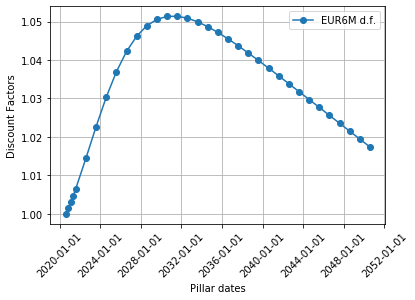
\includegraphics{figures/ex5.5.png}
\end{center}
\end{Answer}





\clearpage
\chapter{Interpolation, Discount Factors and Forward Rates}\label{introduction-to-python---lesson-6}

\begin{Exercise}[title={(Assertion)}]
Python has a useful command called \texttt{assert} which can be used for
checking that a given condition is satisfied, and raising an error if
the condition is not satisfied.

The following line does not cause an error, in fact it does nothing since 1 is lower than 2, hence the condition is met.

\begin{Shaded}
\begin{Highlighting}[]
\ControlFlowTok{assert} \DecValTok{1} \OperatorTok{<} \DecValTok{2}
\end{Highlighting}
\end{Shaded}

This causes an error (the condition is evaluated to false. 

\begin{Shaded}
\begin{Highlighting}[]
\ControlFlowTok{assert} \DecValTok{1} \OperatorTok{>} \DecValTok{2}
\end{Highlighting}
\end{Shaded}

\texttt{assert} can take a second argument with a message to display in case of failure.

\begin{Shaded}
\begin{Highlighting}[]
\ControlFlowTok{assert} \DecValTok{1} \OperatorTok{>} \DecValTok{2}\NormalTok{, }\StringTok{"Two is greater than one"}
\end{Highlighting}
\end{Shaded}

Now takes the \texttt{df} function from Chapter 6 of the Lecture Notes and modify it by adding some assertions to check that:

\begin{itemize}
\tightlist
\item
  the pillar date list contains at least 2 elements;
\item
  the pillar date list has the same length as the discount factor one;
\item
  the first pillar date is equal to the today's date;
\item
  the value date (first argument \texttt{d}) is greater or equal to the first pillar
  date and also less than or equal to the last pillar date.
\end{itemize}

Then try using the function with some invalid data to make sure that your as sertions are correctly checking the desired conditions
\end{Exercise}

\begin{Answer}
\begin{tcolorbox}[size=fbox, boxrule=1pt, colback=cellbackground, colframe=cellborder]
\begin{Verbatim}[commandchars=\\\{\}]
\PY{c+c1}{\PYZsh{} import modules and objects that we need}
\PY{k+kn}{from} \PY{n+nn}{datetime} \PY{k}{import} \PY{n}{date}
\PY{k+kn}{import} \PY{n+nn}{numpy}
\PY{k+kn}{import} \PY{n+nn}{math}

\PY{n}{today\PYZus{}date} \PY{o}{=} \PY{n}{date}\PY{p}{(}\PY{l+m+mi}{2017}\PY{p}{,} \PY{l+m+mi}{10}\PY{p}{,} \PY{l+m+mi}{1}\PY{p}{)}
\PY{n}{pillar\PYZus{}dates} \PY{o}{=} \PY{p}{[}\PY{n}{date}\PY{p}{(}\PY{l+m+mi}{2017}\PY{p}{,} \PY{l+m+mi}{10}\PY{p}{,} \PY{l+m+mi}{1}\PY{p}{)}\PY{p}{,} 
                \PY{n}{date}\PY{p}{(}\PY{l+m+mi}{2018}\PY{p}{,} \PY{l+m+mi}{10}\PY{p}{,} \PY{l+m+mi}{1}\PY{p}{)}\PY{p}{,} 
                \PY{n}{date}\PY{p}{(}\PY{l+m+mi}{2019}\PY{p}{,} \PY{l+m+mi}{10}\PY{p}{,} \PY{l+m+mi}{1}\PY{p}{)}\PY{p}{]}
\PY{n}{discount\PYZus{}factors} \PY{o}{=} \PY{p}{[}\PY{l+m+mf}{1.0}\PY{p}{,} \PY{l+m+mf}{0.95}\PY{p}{,} \PY{l+m+mf}{0.8}\PY{p}{]}

\PY{k}{def} \PY{n+nf}{df}\PY{p}{(}\PY{n}{d, observation_date, pillar_dates, discount_factors}\PY{p}{)}\PY{p}{:}
    \PY{c+c1}{\PYZsh{}\PYZsh{}\PYZsh{}\PYZsh{}\PYZsh{}\PYZsh{}\PYZsh{}\PYZsh{}\PYZsh{}\PYZsh{}\PYZsh{}\PYZsh{}\PYZsh{}\PYZsh{} CHECKS \PYZsh{}\PYZsh{}\PYZsh{}\PYZsh{}\PYZsh{}\PYZsh{}\PYZsh{}\PYZsh{}\PYZsh{}\PYZsh{}\PYZsh{}\PYZsh{}\PYZsh{}\PYZsh{}\PYZsh{}\PYZsh{}}
    \PY{k}{assert} \PY{n+nb}{len}\PY{p}{(}\PY{n}{pillar\PYZus{}dates}\PY{p}{)} \PY{o}{\PYZgt{}}\PY{o}{=} \PY{l+m+mi}{2}\PY{p}{,} \PY{l+s+s2}{\PYZdq{}}\PY{l+s+s2}{ need at least 2 pillar dates}\PY{l+s+s2}{\PYZdq{}}
    
    \PY{k}{assert} \PY{n+nb}{len}\PY{p}{(}\PY{n}{pillar\PYZus{}dates}\PY{p}{)} \PY{o}{==} \PY{n+nb}{len}\PY{p}{(}\PY{n}{discount\PYZus{}factors}\PY{p}{)}\PY{p}{,} \PYZbs{}
        \PY{l+s+s2}{\PYZdq{}}\PY{l+s+s2}{number of pillar dates should be equal to }\PY{l+s+se}{\PYZbs{}}
\PY{l+s+s2}{        the number of pillar discount factors}\PY{l+s+s2}{\PYZdq{}}
    
    \PY{k}{assert} \PY{n}{observation\PYZus{}date} \PY{o}{==} \PY{n}{pillar\PYZus{}dates}\PY{p}{[}\PY{l+m+mi}{0}\PY{p}{]}\PY{p}{,} \PYZbs{}
        \PY{l+s+s2}{\PYZdq{}}\PY{l+s+s2}{first pillar date should be the observation date}\PY{l+s+s2}{\PYZdq{}}
    
    \PY{k}{assert} \PY{n}{pillar\PYZus{}dates}\PY{p}{[}\PY{l+m+mi}{0}\PY{p}{]} \PY{o}{\PYZlt{}}\PY{o}{=} \PY{n}{d} \PY{o}{\PYZlt{}}\PY{o}{=} \PY{n}{pillar\PYZus{}dates}\PY{p}{[}\PY{o}{\PYZhy{}}\PY{l+m+mi}{1}\PY{p}{]}\PY{p}{,} \PYZbs{}
        \PY{l+s+s2}{\PYZdq{}}\PY{l+s+s2}{Invalid value date }\PY{l+s+si}{\PYZpc{}s}\PY{l+s+s2}{\PYZdq{}} \PY{o}{\PYZpc{}} \PY{p}{(}\PY{n}{d}\PY{p}{)}
    \PY{c+c1}{\PYZsh{}\PYZsh{}\PYZsh{}\PYZsh{}\PYZsh{}\PYZsh{}\PYZsh{}\PYZsh{}\PYZsh{}\PYZsh{}\PYZsh{}\PYZsh{}\PYZsh{}\PYZsh{} END OF CHECKS \PYZsh{}\PYZsh{}\PYZsh{}\PYZsh{}\PYZsh{}\PYZsh{}\PYZsh{}\PYZsh{}\PYZsh{}\PYZsh{}\PYZsh{}\PYZsh{}\PYZsh{}\PYZsh{}\PYZsh{}\PYZsh{}}
    
    \PY{n}{log\PYZus{}discount\PYZus{}factors} \PY{o}{=} \PY{p}{[}\PY{p}{]}
    \PY{k}{for} \PY{n}{discount\PYZus{}factor} \PY{o+ow}{in} \PY{n}{discount\PYZus{}factors}\PY{p}{:}
        \PY{n}{log\PYZus{}discount\PYZus{}factors}\PY{o}{.}\PY{n}{append}\PY{p}{(}\PY{n}{math}\PY{o}{.}\PY{n}{log}\PY{p}{(}\PY{n}{discount\PYZus{}factor}\PY{p}{)}\PY{p}{)}
    
    \PY{n}{pillar\PYZus{}days} \PY{o}{=} \PY{p}{[}\PY{p}{]}
    \PY{k}{for} \PY{n}{pillar\PYZus{}date} \PY{o+ow}{in} \PY{n}{pillar\PYZus{}dates}\PY{p}{:}
        \PY{n}{pillar\PYZus{}days}\PY{o}{.}\PY{n}{append}\PY{p}{(}\PY{p}{(}\PY{n}{pillar\PYZus{}date} \PY{o}{\PYZhy{}} \PY{n}{observation\PYZus{}date}\PY{p}{)}\PY{o}{.}\PY{n}{days}\PY{p}{)}
    
    \PY{n}{d\PYZus{}days} \PY{o}{=} \PY{p}{(}\PY{n}{d} \PY{o}{\PYZhy{}} \PY{n}{observation\PYZus{}date}\PY{p}{)}\PY{o}{.}\PY{n}{days}
    
    \PY{n}{interpolated\PYZus{}log\PYZus{}discount\PYZus{}factor} \PY{o}{=} \PYZbs{}
        \PY{n}{numpy}\PY{o}{.}\PY{n}{interp}\PY{p}{(}\PY{n}{d\PYZus{}days}\PY{p}{,} \PY{n}{pillar\PYZus{}days}\PY{p}{,} \PY{n}{log\PYZus{}discount\PYZus{}factors}\PY{p}{)}
    
    \PY{k}{return} \PY{n}{math}\PY{o}{.}\PY{n}{exp}\PY{p}{(}\PY{n}{interpolated\PYZus{}log\PYZus{}discount\PYZus{}factor}\PY{p}{)}

\PY{n}{df}\PY{p}{(}\PY{n}{date}\PY{p}{(}\PY{l+m+mi}{2019}\PY{p}{,} \PY{l+m+mi}{1}\PY{p}{,} \PY{l+m+mi}{1}\PY{p}{), today_date, pillar_dates, discount_factors}\PY{p}{)}

0.9097285910181567
\end{Verbatim}
\end{tcolorbox} 
\end{Answer}

\begin{Exercise}[label={ex:BS3}, title={(Black-Scholes Again)}]
Copy into the file \texttt{finmarkets.py} the function used to compute Black Scholes formula used in Ex.~\ref{ex:BS2}. This is another utility for our financial library. Then repeat Ex.~\ref{ex:BS2} now using the version of the Black and Scholes formula in the \texttt{finmarkets} module.
\end{Exercise}

\begin{Answer}
\begin{tcolorbox}[size=fbox, boxrule=1pt, colback=cellbackground, colframe=cellborder]
\begin{Verbatim}[commandchars=\\\{\}]
\PY{k}{import} \PY{n}{finmarkets}
        
\PY{n}{s} \PY{o}{=} \PY{l+m+mi}{800}
\PY{c+c1}{\PYZsh{} strikes expressed as \PYZpc{} of spot price}
\PY{n}{moneyness} \PY{o}{=} \PY{p}{[} \PY{l+m+mf}{0.5}\PY{p}{,} \PY{l+m+mf}{0.75}\PY{p}{,} \PY{l+m+mf}{0.825}\PY{p}{,} \PYZbs{}
             \PY{l+m+mf}{1.0}\PY{p}{,} \PY{l+m+mf}{1.125}\PY{p}{,} \PY{l+m+mf}{1.25}\PY{p}{,} \PY{l+m+mf}{1.5} \PY{p}{]}
\PY{n}{vol} \PY{o}{=} \PY{l+m+mf}{0.3}
\PY{n}{ttm} \PY{o}{=} \PY{l+m+mf}{0.75}
\PY{n}{r} \PY{o}{=} \PY{l+m+mf}{0.005}

\PY{n}{result} \PY{o}{=} \PY{p}{\PYZob{}}\PY{p}{\PYZcb{}}
\PY{k}{for} \PY{n}{m} \PY{o+ow}{in} \PY{n}{moneyness}\PY{p}{:}
    \PY{n}{result}\PY{p}{[}\PY{n}{s}\PY{o}{*}\PY{n}{m}\PY{p}{]} \PY{o}{=} \PY{n}{finmarkets.call}\PY{p}{(}\PY{n}{s}\PY{p}{,} \PY{n}{m}\PY{o}{*}\PY{n}{s}\PY{p}{,} \PY{n}{r}\PY{p}{,} \PY{n}{vol}\PY{p}{,} \PY{n}{ttm}\PY{p}{)}
\PY{n}{result}

\{400.0: 401.66074527896365,
  600.0: 213.9883852521275,
  660.0: 166.85957363897393,
  800.0: 84.03697017660357,
  900.0: 47.61880394696229,
  1000.0: 25.632722952585738,
  1200.0: 6.655275227771156\}
\end{Verbatim}
\end{tcolorbox}
\end{Answer}

\begin{Exercise}[title={(Discount Curves)}]
  Following the steps outlined in Chapter 6 of the Lecture Notes, implement a \texttt{DiscountCurve} class and add it to \texttt{finmarkets} module. The class should have as attributes the pillar dates and the corresponding discount factors and two methods, one to interpolate discount factors and another to calculate forward rates.
  Finally using that class compute the forward 6M LIBOR coupon using the curves given below in pre and post 2008 crisis way.

\textbf{Input:}
\begin{Shaded}
\begin{Highlighting}[]
\NormalTok{observation_date }\OperatorTok{=}\NormalTok{ date (}\DecValTok{2020}\NormalTok{, }\DecValTok{1}\NormalTok{, }\DecValTok{1}\NormalTok{)}
\NormalTok{t1 }\OperatorTok{=}\NormalTok{ date(}\DecValTok{2020}\NormalTok{,}\DecValTok{4}\NormalTok{, }\DecValTok{1}\NormalTok{)}
\NormalTok{t2 }\OperatorTok{=}\NormalTok{ date(}\DecValTok{2020}\NormalTok{, }\DecValTok{10}\NormalTok{, }\DecValTok{1}\NormalTok{)}

\CommentTok{# for EONIA}
\NormalTok{pillar_dates_eonia }\OperatorTok{=}\NormalTok{ [date(}\DecValTok{2020}\NormalTok{ , }\DecValTok{1}\NormalTok{ ,}\DecValTok{1}\NormalTok{), }
\NormalTok{                      date(}\DecValTok{2021}\NormalTok{, }\DecValTok{1}\NormalTok{, }\DecValTok{1}\NormalTok{), }
\NormalTok{                      date(}\DecValTok{2022}\NormalTok{, }\DecValTok{10}\NormalTok{ ,}\DecValTok{1}\NormalTok{)]}
\NormalTok{discount_factors_eonia }\OperatorTok{=}\NormalTok{ [}\FloatTok{1.0}\NormalTok{, }\FloatTok{0.97}\NormalTok{, }\FloatTok{0.72}\NormalTok{]}

\CommentTok{# for LIBOR 6M}
\NormalTok{pillar_dates_libor }\OperatorTok{=}\NormalTok{ [date(}\DecValTok{2020}\NormalTok{, }\DecValTok{1}\NormalTok{ ,}\DecValTok{1}\NormalTok{), }
\NormalTok{                      date(}\DecValTok{2020}\NormalTok{, }\DecValTok{6}\NormalTok{, }\DecValTok{1}\NormalTok{), }
\NormalTok{                      date(}\DecValTok{2020}\NormalTok{, }\DecValTok{12}\NormalTok{ ,}\DecValTok{1}\NormalTok{)]}
\NormalTok{discount_factors_libor }\OperatorTok{=}\NormalTok{ [}\FloatTok{1.0}\NormalTok{, }\FloatTok{0.95}\NormalTok{, }\FloatTok{0.90}\NormalTok{]}
\end{Highlighting}
\end{Shaded}
\end{Exercise}

\begin{Answer}
\begin{tcolorbox}[size=fbox, boxrule=1pt, pad at break*=1mm,colback=cellbackground, colframe=cellborder]
\begin{Verbatim}[commandchars=\\\{\}]
\PY{k+kn}{import} \PY{n+nn}{math}
\PY{k+kn}{import} \PY{n+nn}{numpy}
\PY{k+kn}{from} \PY{n+nn}{datetime} \PY{k}{import} \PY{n}{date}

\PY{k}{class} \PY{n+nc}{DiscountCurve}\PY{p}{:}

    \PY{k}{def} \PY{n+nf}{\PYZus{}\PYZus{}init\PYZus{}\PYZus{}}\PY{p}{(}\PY{n+nb+bp}{self}\PY{p}{,} \PY{n}{today}\PY{p}{,} \PY{n}{pillar\PYZus{}dates}\PY{p}{,} \PY{n}{discount\PYZus{}factors}\PY{p}{)}\PY{p}{:}
        \PY{n+nb+bp}{self}\PY{o}{.}\PY{n}{today} \PY{o}{=} \PY{n}{today}
        \PY{n+nb+bp}{self}\PY{o}{.}\PY{n}{pillar\PYZus{}dates} \PY{o}{=} \PY{n}{pillar\PYZus{}dates}
        \PY{n+nb+bp}{self}\PY{o}{.}\PY{n}{discount\PYZus{}factors} \PY{o}{=} \PY{n}{discount\PYZus{}factors}

    \PY{k}{def} \PY{n+nf}{df}\PY{p}{(}\PY{n+nb+bp}{self}\PY{p}{,} \PY{n}{d}\PY{p}{)}\PY{p}{:}
        \PY{n}{log\PYZus{}discount\PYZus{}factors} \PY{o}{=} \PYZbs{}
          \PY{p}{[}\PY{n}{math}\PY{o}{.}\PY{n}{log}\PY{p}{(}\PY{n}{discount\PYZus{}factor}\PY{p}{)} 
           \PY{k}{for} \PY{n}{discount\PYZus{}factor} \PY{o+ow}{in} \PY{n+nb+bp}{self}\PY{o}{.}\PY{n}{discount\PYZus{}factors}\PY{p}{]}
        \PY{n}{pillar\PYZus{}days} \PY{o}{=} \PY{p}{[}\PY{p}{(}\PY{n}{pillar\PYZus{}date} \PY{o}{\PYZhy{}} \PY{n+nb+bp}{self}\PY{o}{.}\PY{n}{today}\PY{p}{)}\PY{o}{.}\PY{n}{days} 
                       \PY{k}{for} \PY{n}{pillar\PYZus{}date} \PY{o+ow}{in} \PY{n+nb+bp}{self}\PY{o}{.}\PY{n}{pillar\PYZus{}dates}\PY{p}{]}
        \PY{n}{d\PYZus{}days} \PY{o}{=} \PY{p}{(}\PY{n}{d} \PY{o}{\PYZhy{}} \PY{n+nb+bp}{self}\PY{o}{.}\PY{n}{today}\PY{p}{)}\PY{o}{.}\PY{n}{days}
        \PY{n}{interpolated\PYZus{}log\PYZus{}discount\PYZus{}factor} \PY{o}{=} \PYZbs{}
            \PY{n}{numpy}\PY{o}{.}\PY{n}{interp}\PY{p}{(}\PY{n}{d\PYZus{}days}\PY{p}{,} \PY{n}{pillar\PYZus{}days}\PY{p}{,} \PY{n}{log\PYZus{}discount\PYZus{}factors}\PY{p}{)}
        \PY{k}{return} \PY{n}{math}\PY{o}{.}\PY{n}{exp}\PY{p}{(}\PY{n}{interpolated\PYZus{}log\PYZus{}discount\PYZus{}factor}\PY{p}{)}

    \PY{k}{def} \PY{n+nf}{forward\PYZus{}rate}\PY{p}{(}\PY{n+nb+bp}{self}\PY{p}{,} \PY{n}{d1}\PY{p}{,} \PY{n}{d2}\PY{p}{)}\PY{p}{:}
        \PY{k}{return} \PY{p}{(}\PY{n+nb+bp}{self}\PY{o}{.}\PY{n}{df}\PY{p}{(}\PY{n}{d1}\PY{p}{)} \PY{o}{/} \PY{n+nb+bp}{self}\PY{o}{.}\PY{n}{df}\PY{p}{(}\PY{n}{d2}\PY{p}{)} \PY{o}{\PYZhy{}} \PY{l+m+mf}{1.0}\PY{p}{)} \PY{o}{*} \PYZbs{}
                \PY{p}{(}\PY{l+m+mf}{365.0} \PY{o}{/} \PY{p}{(}\PY{p}{(}\PY{n}{d2} \PY{o}{\PYZhy{}} \PY{n}{d1}\PY{p}{)}\PY{o}{.}\PY{n}{days}\PY{p}{)}\PY{p}{)}
\end{Verbatim}
\end{tcolorbox}

\begin{tcolorbox}[breakable, size=fbox, boxrule=1pt, pad at break*=1mm,colback=cellbackground, colframe=cellborder]
\begin{Verbatim}[commandchars=\\\{\}]
\PY{k+kn}{from} \PY{n+nn}{finmarkets} \PY{k}{import} \PY{n}{DiscountCurve}

\PY{n}{observation\PYZus{}date} \PY{o}{=} \PY{n}{date} \PY{p}{(}\PY{l+m+mi}{2020}\PY{p}{,} \PY{l+m+mi}{1}\PY{p}{,} \PY{l+m+mi}{1}\PY{p}{)}
\PY{n}{t1} \PY{o}{=} \PY{n}{date}\PY{p}{(}\PY{l+m+mi}{2020}\PY{p}{,}\PY{l+m+mi}{4}\PY{p}{,} \PY{l+m+mi}{1}\PY{p}{)}
\PY{n}{t2} \PY{o}{=} \PY{n}{date}\PY{p}{(}\PY{l+m+mi}{2020}\PY{p}{,} \PY{l+m+mi}{10}\PY{p}{,} \PY{l+m+mi}{1}\PY{p}{)}

\PY{c+c1}{\PYZsh{} for EONIA}
\PY{n}{pillar\PYZus{}dates\PYZus{}eonia} \PY{o}{=} \PY{p}{[}\PY{n}{date}\PY{p}{(}\PY{l+m+mi}{2020} \PY{p}{,} \PY{l+m+mi}{1} \PY{p}{,}\PY{l+m+mi}{1}\PY{p}{)}\PY{p}{,} 
                      \PY{n}{date}\PY{p}{(}\PY{l+m+mi}{2021}\PY{p}{,} \PY{l+m+mi}{1}\PY{p}{,} \PY{l+m+mi}{1}\PY{p}{)}\PY{p}{,} 
                      \PY{n}{date}\PY{p}{(}\PY{l+m+mi}{2022}\PY{p}{,} \PY{l+m+mi}{10} \PY{p}{,}\PY{l+m+mi}{1}\PY{p}{)}\PY{p}{]}
\PY{n}{discount\PYZus{}factors\PYZus{}eonia} \PY{o}{=} \PY{p}{[}\PY{l+m+mf}{1.0}\PY{p}{,} \PY{l+m+mf}{0.97}\PY{p}{,} \PY{l+m+mf}{0.72}\PY{p}{]}

\PY{c+c1}{\PYZsh{} for LIBOR 6M}
\PY{n}{pillar\PYZus{}dates\PYZus{}libor} \PY{o}{=} \PY{p}{[}\PY{n}{date}\PY{p}{(}\PY{l+m+mi}{2020}\PY{p}{,} \PY{l+m+mi}{1} \PY{p}{,}\PY{l+m+mi}{1}\PY{p}{)}\PY{p}{,} 
                      \PY{n}{date}\PY{p}{(}\PY{l+m+mi}{2020}\PY{p}{,} \PY{l+m+mi}{6}\PY{p}{,} \PY{l+m+mi}{1}\PY{p}{)}\PY{p}{,} 
                      \PY{n}{date}\PY{p}{(}\PY{l+m+mi}{2020}\PY{p}{,} \PY{l+m+mi}{12} \PY{p}{,}\PY{l+m+mi}{1}\PY{p}{)}\PY{p}{]}
\PY{n}{discount\PYZus{}factors\PYZus{}libor} \PY{o}{=} \PY{p}{[}\PY{l+m+mf}{1.0}\PY{p}{,} \PY{l+m+mf}{0.95}\PY{p}{,} \PY{l+m+mf}{0.90}\PY{p}{]}


\PY{n}{eonia\PYZus{}curve} \PY{o}{=} \PY{n}{DiscountCurve}\PY{p}{(}\PY{n}{observation\PYZus{}date}\PY{p}{,} 
                            \PY{n}{pillar\PYZus{}dates\PYZus{}eonia}\PY{p}{,} 
                            \PY{n}{discount\PYZus{}factors\PYZus{}eonia}\PY{p}{)}
\PY{n}{libor\PYZus{}curve} \PY{o}{=} \PY{n}{DiscountCurve}\PY{p}{(}\PY{n}{observation\PYZus{}date}\PY{p}{,} 
                            \PY{n}{pillar\PYZus{}dates\PYZus{}libor}\PY{p}{,} 
                            \PY{n}{discount\PYZus{}factors\PYZus{}libor}\PY{p}{)}


\PY{n}{npv} \PY{o}{=} \PY{n}{eonia\PYZus{}curve}\PY{o}{.}\PY{n}{df}\PY{p}{(}\PY{n}{t1}\PY{p}{)} \PY{o}{*} \PY{n}{libor\PYZus{}curve}\PY{o}{.}\PY{n}{forward\PYZus{}rate}\PY{p}{(}\PY{n}{t1}\PY{p}{,} \PY{n}{t2}\PY{p}{)}

\PY{c+c1}{\PYZsh{} Compute it in the pre\PYZhy{}2008 way}
\PY{n}{npv\PYZus{}pre2008} \PY{o}{=} \PY{n}{libor\PYZus{}curve}\PY{o}{.}\PY{n}{df}\PY{p}{(}\PY{n}{t1}\PY{p}{)} \PY{o}{*} \PY{n}{libor\PYZus{}curve}\PY{o}{.}\PY{n}{forward\PYZus{}rate}\PY{p}{(}\PY{n}{t1}\PY{p}{,} \PY{n}{t2}\PY{p}{)}

\PY{n+nb}{print} \PY{p}{(}\PY{l+s+s2}{\PYZdq{}}\PY{l+s+s2}{NPV post 2008:}\PY{l+s+s2}{\PYZdq{}}\PY{p}{,} \PY{n}{npv}\PY{p}{)}
\PY{n+nb}{print} \PY{p}{(}\PY{l+s+s2}{\PYZdq{}}\PY{l+s+s2}{NPV pre 2008:}\PY{l+s+s2}{\PYZdq{}}\PY{p}{,} \PY{n}{npv\PYZus{}pre2008}\PY{p}{)}

NPV post 2008: 0.11533243116069992
NPV pre 2008: 0.11269481011359303
\end{Verbatim}
\end{tcolorbox}
\end{Answer}

\begin{Exercise}[title={(Forward Rate Curve)}]
Write a ForwardRateCurve class (for EURIBOR/LIBOR rate curve) which
doesn't compute discount factors but only interplatates forward rates;
then add it to the \texttt{finmarkets} module (this function is used to
define the LIBOR curve needed throughout future lessons).
\end{Exercise}

\begin{Answer}
In this case it is enough to write a new \texttt{class} that has three
attributes: a today date, a set of pillar\_dates and the corresponding
rates. There will be just a single method \texttt{forward\_rate} which
returns the corresponding interpolated rate.

\begin{tcolorbox}[size=fbox, boxrule=1pt, colback=cellbackground, colframe=cellborder]
\begin{Verbatim}[commandchars=\\\{\}]
\PY{k+kn}{import} \PY{n+nn}{numpy}
        
\PY{c+c1}{\PYZsh{} an EURIBOR or LIBOR rate curve}
\PY{c+c1}{\PYZsh{} doesn\PYZsq{}t calculate discount factors, only interpolates forward rates}
\PY{k}{class} \PY{n+nc}{ForwardRateCurve}\PY{p}{(}\PY{n+nb}{object}\PY{p}{)}\PY{p}{:}
   
   \PY{c+c1}{\PYZsh{} the special \PYZus{}\PYZus{}init\PYZus{}\PYZus{} method defines how to}
   \PY{c+c1}{\PYZsh{} construct instances of the class}
   \PY{k}{def} \PY{n+nf}{\PYZus{}\PYZus{}init\PYZus{}\PYZus{}}\PY{p}{(}\PY{n+nb+bp}{self}\PY{p}{,} \PY{n}{pillar\PYZus{}dates}\PY{p}{,} \PY{n}{rates}\PY{p}{)}\PY{p}{:}
       
       \PY{c+c1}{\PYZsh{} we just store the arguments as attributes of the instance}
       \PY{n+nb+bp}{self}\PY{o}{.}\PY{n}{today} \PY{o}{=} \PY{n}{pillar\PYZus{}dates}\PY{p}{[}\PY{l+m+mi}{0}\PY{p}{]}
       \PY{n+nb+bp}{self}\PY{o}{.}\PY{n}{rates} \PY{o}{=} \PY{n}{rates}
       
       \PY{n+nb+bp}{self}\PY{o}{.}\PY{n}{pillar\PYZus{}days} \PY{o}{=} \PY{p}{[}
           \PY{p}{(}\PY{n}{pillar\PYZus{}date} \PY{o}{\PYZhy{}} \PY{n+nb+bp}{self}\PY{o}{.}\PY{n}{today}\PY{p}{)}\PY{o}{.}\PY{n}{days}
           \PY{k}{for} \PY{n}{pillar\PYZus{}date} \PY{o+ow}{in} \PY{n}{pillar\PYZus{}dates}
       \PY{p}{]}
       
       
   \PY{c+c1}{\PYZsh{} interpolates the forward rates stored in the instance}
   \PY{k}{def} \PY{n+nf}{forward\PYZus{}rate}\PY{p}{(}\PY{n+nb+bp}{self}\PY{p}{,} \PY{n}{d}\PY{p}{)}\PY{p}{:}
       \PY{n}{d\PYZus{}days} \PY{o}{=} \PY{p}{(}\PY{n}{d} \PY{o}{\PYZhy{}} \PY{n+nb+bp}{self}\PY{o}{.}\PY{n}{today}\PY{p}{)}\PY{o}{.}\PY{n}{days}
       \PY{k}{return} \PY{n}{numpy}\PY{o}{.}\PY{n}{interp}\PY{p}{(}\PY{n}{d\PYZus{}days}\PY{p}{,} \PY{n+nb+bp}{self}\PY{o}{.}\PY{n}{pillar\PYZus{}days}\PY{p}{,} \PY{n+nb+bp}{self}\PY{o}{.}\PY{n}{rates}\PY{p}{)}
\end{Verbatim}
\end{tcolorbox}
\end{Answer}


  

\clearpage
%\chapter{Interpolation, Discount Factors and Forward Rates}\label{introduction-to-python---lesson-6}

\begin{Exercise}[title={(Assertion)}]
Python has a useful command called \texttt{assert} which can be used for
checking that a given condition is satisfied, and raising an error if
the condition is not satisfied.

The following line does not cause an error, in fact it does nothing since 1 is lower than 2, hence the condition is met.

\begin{Shaded}
\begin{Highlighting}[]
\ControlFlowTok{assert} \DecValTok{1} \OperatorTok{<} \DecValTok{2}
\end{Highlighting}
\end{Shaded}

This causes an error (the condition is evaluated to false. 

\begin{Shaded}
\begin{Highlighting}[]
\ControlFlowTok{assert} \DecValTok{1} \OperatorTok{>} \DecValTok{2}
\end{Highlighting}
\end{Shaded}

\texttt{assert} can take a second argument with a message to display in case of failure.

\begin{Shaded}
\begin{Highlighting}[]
\ControlFlowTok{assert} \DecValTok{1} \OperatorTok{>} \DecValTok{2}\NormalTok{, }\StringTok{"Two is greater than one"}
\end{Highlighting}
\end{Shaded}

Now takes the \texttt{df} function from Chapter 6 of the Lecture Notes and modify it by adding some assertions to check that:

\begin{itemize}
\tightlist
\item
  the pillar date list contains at least 2 elements;
\item
  the pillar date list has the same length as the discount factor one;
\item
  the first pillar date is equal to the today's date;
\item
  the value date (first argument \texttt{d}) is greater or equal to the first pillar
  date and also less than or equal to the last pillar date.
\end{itemize}

Then try using the function with some invalid data to make sure that your as sertions are correctly checking the desired conditions
\end{Exercise}

\begin{Answer}
\begin{tcolorbox}[size=fbox, boxrule=1pt, colback=cellbackground, colframe=cellborder]
\begin{Verbatim}[commandchars=\\\{\}]
\PY{c+c1}{\PYZsh{} import modules and objects that we need}
\PY{k+kn}{from} \PY{n+nn}{datetime} \PY{k}{import} \PY{n}{date}
\PY{k+kn}{import} \PY{n+nn}{numpy}
\PY{k+kn}{import} \PY{n+nn}{math}

\PY{n}{today\PYZus{}date} \PY{o}{=} \PY{n}{date}\PY{p}{(}\PY{l+m+mi}{2017}\PY{p}{,} \PY{l+m+mi}{10}\PY{p}{,} \PY{l+m+mi}{1}\PY{p}{)}
\PY{n}{pillar\PYZus{}dates} \PY{o}{=} \PY{p}{[}\PY{n}{date}\PY{p}{(}\PY{l+m+mi}{2017}\PY{p}{,} \PY{l+m+mi}{10}\PY{p}{,} \PY{l+m+mi}{1}\PY{p}{)}\PY{p}{,} 
                \PY{n}{date}\PY{p}{(}\PY{l+m+mi}{2018}\PY{p}{,} \PY{l+m+mi}{10}\PY{p}{,} \PY{l+m+mi}{1}\PY{p}{)}\PY{p}{,} 
                \PY{n}{date}\PY{p}{(}\PY{l+m+mi}{2019}\PY{p}{,} \PY{l+m+mi}{10}\PY{p}{,} \PY{l+m+mi}{1}\PY{p}{)}\PY{p}{]}
\PY{n}{discount\PYZus{}factors} \PY{o}{=} \PY{p}{[}\PY{l+m+mf}{1.0}\PY{p}{,} \PY{l+m+mf}{0.95}\PY{p}{,} \PY{l+m+mf}{0.8}\PY{p}{]}

\PY{k}{def} \PY{n+nf}{df}\PY{p}{(}\PY{n}{d, observation_date, pillar_dates, discount_factors}\PY{p}{)}\PY{p}{:}
    \PY{c+c1}{\PYZsh{}\PYZsh{}\PYZsh{}\PYZsh{}\PYZsh{}\PYZsh{}\PYZsh{}\PYZsh{}\PYZsh{}\PYZsh{}\PYZsh{}\PYZsh{}\PYZsh{}\PYZsh{} CHECKS \PYZsh{}\PYZsh{}\PYZsh{}\PYZsh{}\PYZsh{}\PYZsh{}\PYZsh{}\PYZsh{}\PYZsh{}\PYZsh{}\PYZsh{}\PYZsh{}\PYZsh{}\PYZsh{}\PYZsh{}\PYZsh{}}
    \PY{k}{assert} \PY{n+nb}{len}\PY{p}{(}\PY{n}{pillar\PYZus{}dates}\PY{p}{)} \PY{o}{\PYZgt{}}\PY{o}{=} \PY{l+m+mi}{2}\PY{p}{,} \PY{l+s+s2}{\PYZdq{}}\PY{l+s+s2}{ need at least 2 pillar dates}\PY{l+s+s2}{\PYZdq{}}
    
    \PY{k}{assert} \PY{n+nb}{len}\PY{p}{(}\PY{n}{pillar\PYZus{}dates}\PY{p}{)} \PY{o}{==} \PY{n+nb}{len}\PY{p}{(}\PY{n}{discount\PYZus{}factors}\PY{p}{)}\PY{p}{,} \PYZbs{}
        \PY{l+s+s2}{\PYZdq{}}\PY{l+s+s2}{number of pillar dates should be equal to }\PY{l+s+se}{\PYZbs{}}
\PY{l+s+s2}{        the number of pillar discount factors}\PY{l+s+s2}{\PYZdq{}}
    
    \PY{k}{assert} \PY{n}{observation\PYZus{}date} \PY{o}{==} \PY{n}{pillar\PYZus{}dates}\PY{p}{[}\PY{l+m+mi}{0}\PY{p}{]}\PY{p}{,} \PYZbs{}
        \PY{l+s+s2}{\PYZdq{}}\PY{l+s+s2}{first pillar date should be the observation date}\PY{l+s+s2}{\PYZdq{}}
    
    \PY{k}{assert} \PY{n}{pillar\PYZus{}dates}\PY{p}{[}\PY{l+m+mi}{0}\PY{p}{]} \PY{o}{\PYZlt{}}\PY{o}{=} \PY{n}{d} \PY{o}{\PYZlt{}}\PY{o}{=} \PY{n}{pillar\PYZus{}dates}\PY{p}{[}\PY{o}{\PYZhy{}}\PY{l+m+mi}{1}\PY{p}{]}\PY{p}{,} \PYZbs{}
        \PY{l+s+s2}{\PYZdq{}}\PY{l+s+s2}{Invalid value date }\PY{l+s+si}{\PYZpc{}s}\PY{l+s+s2}{\PYZdq{}} \PY{o}{\PYZpc{}} \PY{p}{(}\PY{n}{d}\PY{p}{)}
    \PY{c+c1}{\PYZsh{}\PYZsh{}\PYZsh{}\PYZsh{}\PYZsh{}\PYZsh{}\PYZsh{}\PYZsh{}\PYZsh{}\PYZsh{}\PYZsh{}\PYZsh{}\PYZsh{}\PYZsh{} END OF CHECKS \PYZsh{}\PYZsh{}\PYZsh{}\PYZsh{}\PYZsh{}\PYZsh{}\PYZsh{}\PYZsh{}\PYZsh{}\PYZsh{}\PYZsh{}\PYZsh{}\PYZsh{}\PYZsh{}\PYZsh{}\PYZsh{}}
    
    \PY{n}{log\PYZus{}discount\PYZus{}factors} \PY{o}{=} \PY{p}{[}\PY{p}{]}
    \PY{k}{for} \PY{n}{discount\PYZus{}factor} \PY{o+ow}{in} \PY{n}{discount\PYZus{}factors}\PY{p}{:}
        \PY{n}{log\PYZus{}discount\PYZus{}factors}\PY{o}{.}\PY{n}{append}\PY{p}{(}\PY{n}{math}\PY{o}{.}\PY{n}{log}\PY{p}{(}\PY{n}{discount\PYZus{}factor}\PY{p}{)}\PY{p}{)}
    
    \PY{n}{pillar\PYZus{}days} \PY{o}{=} \PY{p}{[}\PY{p}{]}
    \PY{k}{for} \PY{n}{pillar\PYZus{}date} \PY{o+ow}{in} \PY{n}{pillar\PYZus{}dates}\PY{p}{:}
        \PY{n}{pillar\PYZus{}days}\PY{o}{.}\PY{n}{append}\PY{p}{(}\PY{p}{(}\PY{n}{pillar\PYZus{}date} \PY{o}{\PYZhy{}} \PY{n}{observation\PYZus{}date}\PY{p}{)}\PY{o}{.}\PY{n}{days}\PY{p}{)}
    
    \PY{n}{d\PYZus{}days} \PY{o}{=} \PY{p}{(}\PY{n}{d} \PY{o}{\PYZhy{}} \PY{n}{observation\PYZus{}date}\PY{p}{)}\PY{o}{.}\PY{n}{days}
    
    \PY{n}{interpolated\PYZus{}log\PYZus{}discount\PYZus{}factor} \PY{o}{=} \PYZbs{}
        \PY{n}{numpy}\PY{o}{.}\PY{n}{interp}\PY{p}{(}\PY{n}{d\PYZus{}days}\PY{p}{,} \PY{n}{pillar\PYZus{}days}\PY{p}{,} \PY{n}{log\PYZus{}discount\PYZus{}factors}\PY{p}{)}
    
    \PY{k}{return} \PY{n}{math}\PY{o}{.}\PY{n}{exp}\PY{p}{(}\PY{n}{interpolated\PYZus{}log\PYZus{}discount\PYZus{}factor}\PY{p}{)}

\PY{n}{df}\PY{p}{(}\PY{n}{date}\PY{p}{(}\PY{l+m+mi}{2019}\PY{p}{,} \PY{l+m+mi}{1}\PY{p}{,} \PY{l+m+mi}{1}\PY{p}{), today_date, pillar_dates, discount_factors}\PY{p}{)}

0.9097285910181567
\end{Verbatim}
\end{tcolorbox} 
\end{Answer}

\begin{Exercise}[label={ex:BS3}, title={(Black-Scholes Again)}]
Copy into the file \texttt{finmarkets.py} the function used to compute Black Scholes formula used in Ex.~\ref{ex:BS2}. This is another utility for our financial library. Then repeat Ex.~\ref{ex:BS2} now using the version of the Black and Scholes formula in the \texttt{finmarkets} module.
\end{Exercise}

\begin{Answer}
\begin{tcolorbox}[size=fbox, boxrule=1pt, colback=cellbackground, colframe=cellborder]
\begin{Verbatim}[commandchars=\\\{\}]
\PY{k}{import} \PY{n}{finmarkets}
        
\PY{n}{s} \PY{o}{=} \PY{l+m+mi}{800}
\PY{c+c1}{\PYZsh{} strikes expressed as \PYZpc{} of spot price}
\PY{n}{moneyness} \PY{o}{=} \PY{p}{[} \PY{l+m+mf}{0.5}\PY{p}{,} \PY{l+m+mf}{0.75}\PY{p}{,} \PY{l+m+mf}{0.825}\PY{p}{,} \PYZbs{}
             \PY{l+m+mf}{1.0}\PY{p}{,} \PY{l+m+mf}{1.125}\PY{p}{,} \PY{l+m+mf}{1.25}\PY{p}{,} \PY{l+m+mf}{1.5} \PY{p}{]}
\PY{n}{vol} \PY{o}{=} \PY{l+m+mf}{0.3}
\PY{n}{ttm} \PY{o}{=} \PY{l+m+mf}{0.75}
\PY{n}{r} \PY{o}{=} \PY{l+m+mf}{0.005}

\PY{n}{result} \PY{o}{=} \PY{p}{\PYZob{}}\PY{p}{\PYZcb{}}
\PY{k}{for} \PY{n}{m} \PY{o+ow}{in} \PY{n}{moneyness}\PY{p}{:}
    \PY{n}{result}\PY{p}{[}\PY{n}{s}\PY{o}{*}\PY{n}{m}\PY{p}{]} \PY{o}{=} \PY{n}{finmarkets.call}\PY{p}{(}\PY{n}{s}\PY{p}{,} \PY{n}{m}\PY{o}{*}\PY{n}{s}\PY{p}{,} \PY{n}{r}\PY{p}{,} \PY{n}{vol}\PY{p}{,} \PY{n}{ttm}\PY{p}{)}
\PY{n}{result}

\{400.0: 401.66074527896365,
  600.0: 213.9883852521275,
  660.0: 166.85957363897393,
  800.0: 84.03697017660357,
  900.0: 47.61880394696229,
  1000.0: 25.632722952585738,
  1200.0: 6.655275227771156\}
\end{Verbatim}
\end{tcolorbox}
\end{Answer}

\begin{Exercise}[title={(Discount Curves)}]
  Following the steps outlined in Chapter 6 of the Lecture Notes, implement a \texttt{DiscountCurve} class and add it to \texttt{finmarkets} module. The class should have as attributes the pillar dates and the corresponding discount factors and two methods, one to interpolate discount factors and another to calculate forward rates.
  Finally using that class compute the forward 6M LIBOR coupon using the curves given below in pre and post 2008 crisis way.

\textbf{Input:}
\begin{Shaded}
\begin{Highlighting}[]
\NormalTok{observation_date }\OperatorTok{=}\NormalTok{ date (}\DecValTok{2020}\NormalTok{, }\DecValTok{1}\NormalTok{, }\DecValTok{1}\NormalTok{)}
\NormalTok{t1 }\OperatorTok{=}\NormalTok{ date(}\DecValTok{2020}\NormalTok{,}\DecValTok{4}\NormalTok{, }\DecValTok{1}\NormalTok{)}
\NormalTok{t2 }\OperatorTok{=}\NormalTok{ date(}\DecValTok{2020}\NormalTok{, }\DecValTok{10}\NormalTok{, }\DecValTok{1}\NormalTok{)}

\CommentTok{# for EONIA}
\NormalTok{pillar_dates_eonia }\OperatorTok{=}\NormalTok{ [date(}\DecValTok{2020}\NormalTok{ , }\DecValTok{1}\NormalTok{ ,}\DecValTok{1}\NormalTok{), }
\NormalTok{                      date(}\DecValTok{2021}\NormalTok{, }\DecValTok{1}\NormalTok{, }\DecValTok{1}\NormalTok{), }
\NormalTok{                      date(}\DecValTok{2022}\NormalTok{, }\DecValTok{10}\NormalTok{ ,}\DecValTok{1}\NormalTok{)]}
\NormalTok{discount_factors_eonia }\OperatorTok{=}\NormalTok{ [}\FloatTok{1.0}\NormalTok{, }\FloatTok{0.97}\NormalTok{, }\FloatTok{0.72}\NormalTok{]}

\CommentTok{# for LIBOR 6M}
\NormalTok{pillar_dates_libor }\OperatorTok{=}\NormalTok{ [date(}\DecValTok{2020}\NormalTok{, }\DecValTok{1}\NormalTok{ ,}\DecValTok{1}\NormalTok{), }
\NormalTok{                      date(}\DecValTok{2020}\NormalTok{, }\DecValTok{6}\NormalTok{, }\DecValTok{1}\NormalTok{), }
\NormalTok{                      date(}\DecValTok{2020}\NormalTok{, }\DecValTok{12}\NormalTok{ ,}\DecValTok{1}\NormalTok{)]}
\NormalTok{discount_factors_libor }\OperatorTok{=}\NormalTok{ [}\FloatTok{1.0}\NormalTok{, }\FloatTok{0.95}\NormalTok{, }\FloatTok{0.90}\NormalTok{]}
\end{Highlighting}
\end{Shaded}
\end{Exercise}

\begin{Answer}
\begin{tcolorbox}[size=fbox, boxrule=1pt, pad at break*=1mm,colback=cellbackground, colframe=cellborder]
\begin{Verbatim}[commandchars=\\\{\}]
\PY{k+kn}{import} \PY{n+nn}{math}
\PY{k+kn}{import} \PY{n+nn}{numpy}
\PY{k+kn}{from} \PY{n+nn}{datetime} \PY{k}{import} \PY{n}{date}

\PY{k}{class} \PY{n+nc}{DiscountCurve}\PY{p}{:}

    \PY{k}{def} \PY{n+nf}{\PYZus{}\PYZus{}init\PYZus{}\PYZus{}}\PY{p}{(}\PY{n+nb+bp}{self}\PY{p}{,} \PY{n}{today}\PY{p}{,} \PY{n}{pillar\PYZus{}dates}\PY{p}{,} \PY{n}{discount\PYZus{}factors}\PY{p}{)}\PY{p}{:}
        \PY{n+nb+bp}{self}\PY{o}{.}\PY{n}{today} \PY{o}{=} \PY{n}{today}
        \PY{n+nb+bp}{self}\PY{o}{.}\PY{n}{pillar\PYZus{}dates} \PY{o}{=} \PY{n}{pillar\PYZus{}dates}
        \PY{n+nb+bp}{self}\PY{o}{.}\PY{n}{discount\PYZus{}factors} \PY{o}{=} \PY{n}{discount\PYZus{}factors}

    \PY{k}{def} \PY{n+nf}{df}\PY{p}{(}\PY{n+nb+bp}{self}\PY{p}{,} \PY{n}{d}\PY{p}{)}\PY{p}{:}
        \PY{n}{log\PYZus{}discount\PYZus{}factors} \PY{o}{=} \PYZbs{}
          \PY{p}{[}\PY{n}{math}\PY{o}{.}\PY{n}{log}\PY{p}{(}\PY{n}{discount\PYZus{}factor}\PY{p}{)} 
           \PY{k}{for} \PY{n}{discount\PYZus{}factor} \PY{o+ow}{in} \PY{n+nb+bp}{self}\PY{o}{.}\PY{n}{discount\PYZus{}factors}\PY{p}{]}
        \PY{n}{pillar\PYZus{}days} \PY{o}{=} \PY{p}{[}\PY{p}{(}\PY{n}{pillar\PYZus{}date} \PY{o}{\PYZhy{}} \PY{n+nb+bp}{self}\PY{o}{.}\PY{n}{today}\PY{p}{)}\PY{o}{.}\PY{n}{days} 
                       \PY{k}{for} \PY{n}{pillar\PYZus{}date} \PY{o+ow}{in} \PY{n+nb+bp}{self}\PY{o}{.}\PY{n}{pillar\PYZus{}dates}\PY{p}{]}
        \PY{n}{d\PYZus{}days} \PY{o}{=} \PY{p}{(}\PY{n}{d} \PY{o}{\PYZhy{}} \PY{n+nb+bp}{self}\PY{o}{.}\PY{n}{today}\PY{p}{)}\PY{o}{.}\PY{n}{days}
        \PY{n}{interpolated\PYZus{}log\PYZus{}discount\PYZus{}factor} \PY{o}{=} \PYZbs{}
            \PY{n}{numpy}\PY{o}{.}\PY{n}{interp}\PY{p}{(}\PY{n}{d\PYZus{}days}\PY{p}{,} \PY{n}{pillar\PYZus{}days}\PY{p}{,} \PY{n}{log\PYZus{}discount\PYZus{}factors}\PY{p}{)}
        \PY{k}{return} \PY{n}{math}\PY{o}{.}\PY{n}{exp}\PY{p}{(}\PY{n}{interpolated\PYZus{}log\PYZus{}discount\PYZus{}factor}\PY{p}{)}

    \PY{k}{def} \PY{n+nf}{forward\PYZus{}rate}\PY{p}{(}\PY{n+nb+bp}{self}\PY{p}{,} \PY{n}{d1}\PY{p}{,} \PY{n}{d2}\PY{p}{)}\PY{p}{:}
        \PY{k}{return} \PY{p}{(}\PY{n+nb+bp}{self}\PY{o}{.}\PY{n}{df}\PY{p}{(}\PY{n}{d1}\PY{p}{)} \PY{o}{/} \PY{n+nb+bp}{self}\PY{o}{.}\PY{n}{df}\PY{p}{(}\PY{n}{d2}\PY{p}{)} \PY{o}{\PYZhy{}} \PY{l+m+mf}{1.0}\PY{p}{)} \PY{o}{*} \PYZbs{}
                \PY{p}{(}\PY{l+m+mf}{365.0} \PY{o}{/} \PY{p}{(}\PY{p}{(}\PY{n}{d2} \PY{o}{\PYZhy{}} \PY{n}{d1}\PY{p}{)}\PY{o}{.}\PY{n}{days}\PY{p}{)}\PY{p}{)}
\end{Verbatim}
\end{tcolorbox}

\begin{tcolorbox}[breakable, size=fbox, boxrule=1pt, pad at break*=1mm,colback=cellbackground, colframe=cellborder]
\begin{Verbatim}[commandchars=\\\{\}]
\PY{k+kn}{from} \PY{n+nn}{finmarkets} \PY{k}{import} \PY{n}{DiscountCurve}

\PY{n}{observation\PYZus{}date} \PY{o}{=} \PY{n}{date} \PY{p}{(}\PY{l+m+mi}{2020}\PY{p}{,} \PY{l+m+mi}{1}\PY{p}{,} \PY{l+m+mi}{1}\PY{p}{)}
\PY{n}{t1} \PY{o}{=} \PY{n}{date}\PY{p}{(}\PY{l+m+mi}{2020}\PY{p}{,}\PY{l+m+mi}{4}\PY{p}{,} \PY{l+m+mi}{1}\PY{p}{)}
\PY{n}{t2} \PY{o}{=} \PY{n}{date}\PY{p}{(}\PY{l+m+mi}{2020}\PY{p}{,} \PY{l+m+mi}{10}\PY{p}{,} \PY{l+m+mi}{1}\PY{p}{)}

\PY{c+c1}{\PYZsh{} for EONIA}
\PY{n}{pillar\PYZus{}dates\PYZus{}eonia} \PY{o}{=} \PY{p}{[}\PY{n}{date}\PY{p}{(}\PY{l+m+mi}{2020} \PY{p}{,} \PY{l+m+mi}{1} \PY{p}{,}\PY{l+m+mi}{1}\PY{p}{)}\PY{p}{,} 
                      \PY{n}{date}\PY{p}{(}\PY{l+m+mi}{2021}\PY{p}{,} \PY{l+m+mi}{1}\PY{p}{,} \PY{l+m+mi}{1}\PY{p}{)}\PY{p}{,} 
                      \PY{n}{date}\PY{p}{(}\PY{l+m+mi}{2022}\PY{p}{,} \PY{l+m+mi}{10} \PY{p}{,}\PY{l+m+mi}{1}\PY{p}{)}\PY{p}{]}
\PY{n}{discount\PYZus{}factors\PYZus{}eonia} \PY{o}{=} \PY{p}{[}\PY{l+m+mf}{1.0}\PY{p}{,} \PY{l+m+mf}{0.97}\PY{p}{,} \PY{l+m+mf}{0.72}\PY{p}{]}

\PY{c+c1}{\PYZsh{} for LIBOR 6M}
\PY{n}{pillar\PYZus{}dates\PYZus{}libor} \PY{o}{=} \PY{p}{[}\PY{n}{date}\PY{p}{(}\PY{l+m+mi}{2020}\PY{p}{,} \PY{l+m+mi}{1} \PY{p}{,}\PY{l+m+mi}{1}\PY{p}{)}\PY{p}{,} 
                      \PY{n}{date}\PY{p}{(}\PY{l+m+mi}{2020}\PY{p}{,} \PY{l+m+mi}{6}\PY{p}{,} \PY{l+m+mi}{1}\PY{p}{)}\PY{p}{,} 
                      \PY{n}{date}\PY{p}{(}\PY{l+m+mi}{2020}\PY{p}{,} \PY{l+m+mi}{12} \PY{p}{,}\PY{l+m+mi}{1}\PY{p}{)}\PY{p}{]}
\PY{n}{discount\PYZus{}factors\PYZus{}libor} \PY{o}{=} \PY{p}{[}\PY{l+m+mf}{1.0}\PY{p}{,} \PY{l+m+mf}{0.95}\PY{p}{,} \PY{l+m+mf}{0.90}\PY{p}{]}


\PY{n}{eonia\PYZus{}curve} \PY{o}{=} \PY{n}{DiscountCurve}\PY{p}{(}\PY{n}{observation\PYZus{}date}\PY{p}{,} 
                            \PY{n}{pillar\PYZus{}dates\PYZus{}eonia}\PY{p}{,} 
                            \PY{n}{discount\PYZus{}factors\PYZus{}eonia}\PY{p}{)}
\PY{n}{libor\PYZus{}curve} \PY{o}{=} \PY{n}{DiscountCurve}\PY{p}{(}\PY{n}{observation\PYZus{}date}\PY{p}{,} 
                            \PY{n}{pillar\PYZus{}dates\PYZus{}libor}\PY{p}{,} 
                            \PY{n}{discount\PYZus{}factors\PYZus{}libor}\PY{p}{)}


\PY{n}{npv} \PY{o}{=} \PY{n}{eonia\PYZus{}curve}\PY{o}{.}\PY{n}{df}\PY{p}{(}\PY{n}{t1}\PY{p}{)} \PY{o}{*} \PY{n}{libor\PYZus{}curve}\PY{o}{.}\PY{n}{forward\PYZus{}rate}\PY{p}{(}\PY{n}{t1}\PY{p}{,} \PY{n}{t2}\PY{p}{)}

\PY{c+c1}{\PYZsh{} Compute it in the pre\PYZhy{}2008 way}
\PY{n}{npv\PYZus{}pre2008} \PY{o}{=} \PY{n}{libor\PYZus{}curve}\PY{o}{.}\PY{n}{df}\PY{p}{(}\PY{n}{t1}\PY{p}{)} \PY{o}{*} \PY{n}{libor\PYZus{}curve}\PY{o}{.}\PY{n}{forward\PYZus{}rate}\PY{p}{(}\PY{n}{t1}\PY{p}{,} \PY{n}{t2}\PY{p}{)}

\PY{n+nb}{print} \PY{p}{(}\PY{l+s+s2}{\PYZdq{}}\PY{l+s+s2}{NPV post 2008:}\PY{l+s+s2}{\PYZdq{}}\PY{p}{,} \PY{n}{npv}\PY{p}{)}
\PY{n+nb}{print} \PY{p}{(}\PY{l+s+s2}{\PYZdq{}}\PY{l+s+s2}{NPV pre 2008:}\PY{l+s+s2}{\PYZdq{}}\PY{p}{,} \PY{n}{npv\PYZus{}pre2008}\PY{p}{)}

NPV post 2008: 0.11533243116069992
NPV pre 2008: 0.11269481011359303
\end{Verbatim}
\end{tcolorbox}
\end{Answer}

\begin{Exercise}[title={(Forward Rate Curve)}]
Write a ForwardRateCurve class (for EURIBOR/LIBOR rate curve) which
doesn't compute discount factors but only interplatates forward rates;
then add it to the \texttt{finmarkets} module (this function is used to
define the LIBOR curve needed throughout future lessons).
\end{Exercise}

\begin{Answer}
In this case it is enough to write a new \texttt{class} that has three
attributes: a today date, a set of pillar\_dates and the corresponding
rates. There will be just a single method \texttt{forward\_rate} which
returns the corresponding interpolated rate.

\begin{tcolorbox}[size=fbox, boxrule=1pt, colback=cellbackground, colframe=cellborder]
\begin{Verbatim}[commandchars=\\\{\}]
\PY{k+kn}{import} \PY{n+nn}{numpy}
        
\PY{c+c1}{\PYZsh{} an EURIBOR or LIBOR rate curve}
\PY{c+c1}{\PYZsh{} doesn\PYZsq{}t calculate discount factors, only interpolates forward rates}
\PY{k}{class} \PY{n+nc}{ForwardRateCurve}\PY{p}{(}\PY{n+nb}{object}\PY{p}{)}\PY{p}{:}
   
   \PY{c+c1}{\PYZsh{} the special \PYZus{}\PYZus{}init\PYZus{}\PYZus{} method defines how to}
   \PY{c+c1}{\PYZsh{} construct instances of the class}
   \PY{k}{def} \PY{n+nf}{\PYZus{}\PYZus{}init\PYZus{}\PYZus{}}\PY{p}{(}\PY{n+nb+bp}{self}\PY{p}{,} \PY{n}{pillar\PYZus{}dates}\PY{p}{,} \PY{n}{rates}\PY{p}{)}\PY{p}{:}
       
       \PY{c+c1}{\PYZsh{} we just store the arguments as attributes of the instance}
       \PY{n+nb+bp}{self}\PY{o}{.}\PY{n}{today} \PY{o}{=} \PY{n}{pillar\PYZus{}dates}\PY{p}{[}\PY{l+m+mi}{0}\PY{p}{]}
       \PY{n+nb+bp}{self}\PY{o}{.}\PY{n}{rates} \PY{o}{=} \PY{n}{rates}
       
       \PY{n+nb+bp}{self}\PY{o}{.}\PY{n}{pillar\PYZus{}days} \PY{o}{=} \PY{p}{[}
           \PY{p}{(}\PY{n}{pillar\PYZus{}date} \PY{o}{\PYZhy{}} \PY{n+nb+bp}{self}\PY{o}{.}\PY{n}{today}\PY{p}{)}\PY{o}{.}\PY{n}{days}
           \PY{k}{for} \PY{n}{pillar\PYZus{}date} \PY{o+ow}{in} \PY{n}{pillar\PYZus{}dates}
       \PY{p}{]}
       
       
   \PY{c+c1}{\PYZsh{} interpolates the forward rates stored in the instance}
   \PY{k}{def} \PY{n+nf}{forward\PYZus{}rate}\PY{p}{(}\PY{n+nb+bp}{self}\PY{p}{,} \PY{n}{d}\PY{p}{)}\PY{p}{:}
       \PY{n}{d\PYZus{}days} \PY{o}{=} \PY{p}{(}\PY{n}{d} \PY{o}{\PYZhy{}} \PY{n+nb+bp}{self}\PY{o}{.}\PY{n}{today}\PY{p}{)}\PY{o}{.}\PY{n}{days}
       \PY{k}{return} \PY{n}{numpy}\PY{o}{.}\PY{n}{interp}\PY{p}{(}\PY{n}{d\PYZus{}days}\PY{p}{,} \PY{n+nb+bp}{self}\PY{o}{.}\PY{n}{pillar\PYZus{}days}\PY{p}{,} \PY{n+nb+bp}{self}\PY{o}{.}\PY{n}{rates}\PY{p}{)}
\end{Verbatim}
\end{tcolorbox}
\end{Answer}


  

%\clearpage
%\chapter{Monte Carlo Simulation}\label{introduction-to-python---lesson-8}

\begin{Exercise}[title={(Dice Simulation)}]
Using the function \texttt{randint} of the module \texttt{random} make a
Monte Carlo simulation of rolling three dices to check the probability
of getting the same values on the three of them.

From the probability theory you should expect:

\[P_{d1=d2=d3} = \frac{1}{6}\cdot\frac{1}{6}\cdot\frac{1}{6}\cdot 6 = \frac{1}{36} = 0.0278\]
\end{Exercise}
\begin{Answer}
\begin{tcolorbox}[size=fbox, boxrule=1pt, colback=cellbackground, colframe=cellborder]
\begin{Verbatim}[commandchars=\\\{\}]
\PY{k+kn}{from} \PY{n+nn}{random} \PY{k}{import} \PY{n}{seed}\PY{p}{,} \PY{n}{randint}
        
\PY{n}{seed}\PY{p}{(}\PY{l+m+mi}{1}\PY{p}{)}
        
\PY{n}{trials} \PY{o}{=} \PY{l+m+mi}{10000000}
\PY{n}{success} \PY{o}{=} \PY{l+m+mi}{0}
\PY{k}{for} \PY{n}{\PYZus{}} \PY{o+ow}{in} \PY{n+nb}{range}\PY{p}{(}\PY{n}{trials}\PY{p}{)}\PY{p}{:}{6}\PY{p}{)}\PY{p}{,} \PY{n}{randint}\PY{p}{(}\PY{l+m+mi}{1}\PY{p}{,} \PY{l+m+mi}{6}\PY{p}{)}\PY{p}{,} \PY{n}{randint}\PY{p}{(}\PY{l+m+mi}{1}\PY{p}{,} \PY{l+m+mi}{6}\PY{p}{)}    
    \PY{k}{if} \PY{n}{d1} \PY{o}{==} \PY{n}{d2} \PY{o+ow}{and} \PY{n}{d2} \PY{o}{==} \PY{n}{d3}\PY{p}{:}
        \PY{n}{success} \PY{o}{+}\PY{o}{=} \PY{l+m+mi}{1}
    
\PY{n+nb}{print} \PY{p}{(}\PY{l+s+s2}{\PYZdq{}}\PY{l+s+s2}{The probability to get three equal dice is }\PY{l+s+si}{\PYZob{}:.4f\PYZcb{}}\PY{l+s+s2}{\PYZdq{}}\PY{o}{.}\PY{n}{format}\PY{p}{(}\PY{n}{success}\PY{o}{/}\PY{n}{trials}\PY{p}{)}\PY{p}{)}
        
The probability to get three equal dice is 0.0278
\end{Verbatim}
\end{tcolorbox}
\end{Answer}

\begin{Exercise}[title={(Dice simulation II)}]
Two fair dice are rolled, find the probability that their sum is:
\begin{enumerate}
	\item equal to 1
	\item equal to 4
	\item less than 13
\end{enumerate}
	
\textbf{Hint:} the possible combinations of the outcomes of two dice are 36 (to realize it you can simply think that for each one of the six faces of the first die you have six possible faces of the second hence $6\cdot 6=36$). It is not possible to get 1 since 	the dice have no face with 0 so the first probability should come out 0. The sum of the two dice is always less than 13 (the maximum is 12\ldots) so the answer to point 3 is 1. We can get a sum of 4 in 3 cases (1-3, 3-1 or 2-2) so the expected probability is $3/36=1/12=0.0833$
\end{Exercise}

\begin{Answer}
\begin{tcolorbox}[size=fbox, boxrule=1pt, colback=cellbackground, colframe=cellborder]
\begin{Verbatim}[commandchars=\\\{\}]
\PY{k+kn}{import} \PY{n+nn}{random}
	
\PY{n}{random}\PY{o}{.}\PY{n}{seed}\PY{p}{(}\PY{l+m+mi}{1}\PY{p}{)}
	
\PY{n}{successes} \PY{o}{=} \PY{p}{\PYZob{}}\PY{l+s+s2}{\PYZdq{}}\PY{l+s+s2}{=1}\PY{l+s+s2}{\PYZdq{}}\PY{p}{:}\PY{l+m+mf}{0.0}\PY{p}{,} \PY{l+s+s2}{\PYZdq{}}\PY{l+s+s2}{=4}\PY{l+s+s2}{\PYZdq{}}\PY{p}{:}\PY{l+m+mf}{0.0}\PY{p}{,} \PY{l+s+s2}{\PYZdq{}}\PY{l+s+s2}{\PYZlt{}13}\PY{l+s+s2}{\PYZdq{}}\PY{p}{:}\PY{l+m+mf}{0.0}\PY{p}{\PYZcb{}}
\PY{n}{trials} \PY{o}{=} \PY{l+m+mi}{100000}
\PY{k}{for} \PY{n}{\PYZus{}} \PY{o+ow}{in} \PY{n+nb}{range}\PY{p}{(}\PY{n}{trials}\PY{p}{)}\PY{p}{:}
    \PY{n}{d1} \PY{o}{=} \PY{n}{random}\PY{o}{.}\PY{n}{randint}\PY{p}{(}\PY{l+m+mi}{1}\PY{p}{,} \PY{l+m+mi}{6}\PY{p}{)}
    \PY{n}{d2} \PY{o}{=} \PY{n}{random}\PY{o}{.}\PY{n}{randint}\PY{p}{(}\PY{l+m+mi}{1}\PY{p}{,} \PY{l+m+mi}{6}\PY{p}{)}
    \PY{k}{if} \PY{p}{(}\PY{n}{d1} \PY{o}{+} \PY{n}{d2}\PY{p}{)} \PY{o}{==} \PY{l+m+mi}{1}\PY{p}{:}
        \PY{n}{successes}\PY{p}{[}\PY{l+s+s2}{\PYZdq{}}\PY{l+s+s2}{=0}\PY{l+s+s2}{\PYZdq{}}\PY{p}{]} \PY{o}{+}\PY{o}{=} \PY{l+m+mf}{1.0}
    \PY{k}{if} \PY{p}{(}\PY{n}{d1} \PY{o}{+} \PY{n}{d2}\PY{p}{)} \PY{o}{==} \PY{l+m+mi}{4}\PY{p}{:}
        \PY{n}{successes}\PY{p}{[}\PY{l+s+s2}{\PYZdq{}}\PY{l+s+s2}{=4}\PY{l+s+s2}{\PYZdq{}}\PY{p}{]} \PY{o}{+}\PY{o}{=} \PY{l+m+mf}{1.0}
    \PY{k}{if} \PY{p}{(}\PY{n}{d1} \PY{o}{+} \PY{n}{d2}\PY{p}{)} \PY{o}{\PYZlt{}} \PY{l+m+mi}{13}\PY{p}{:}
        \PY{n}{successes}\PY{p}{[}\PY{l+s+s2}{\PYZdq{}}\PY{l+s+s2}{\PYZlt{}13}\PY{l+s+s2}{\PYZdq{}}\PY{p}{]} \PY{o}{+}\PY{o}{=} \PY{l+m+mf}{1.0}
	
\PY{k}{for} \PY{n}{k}\PY{p}{,}\PY{n}{v} \PY{o+ow}{in} \PY{n}{successes}\PY{o}{.}\PY{n}{items}\PY{p}{(}\PY{p}{)}\PY{p}{:}
    \PY{n+nb}{print} \PY{p}{(}\PY{l+s+s2}{\PYZdq{}}\PY{l+s+s2}{P(}\PY{l+s+si}{\PYZob{}\PYZcb{}}\PY{l+s+s2}{): }\PY{l+s+si}{\PYZob{}:.3f\PYZcb{}}\PY{l+s+s2}{\PYZdq{}}\PY{o}{.}\PY{n}{format}\PY{p}{(}\PY{n}{k}\PY{p}{,} \PY{n}{v}\PY{o}{/}\PY{n}{trials}\PY{p}{)}\PY{p}{)}
	
P(=1): 0.000
P(=4): 0.084
P(<13): 1.000
\end{Verbatim}
\end{tcolorbox}
\end{Answer}

\begin{Exercise}[title={(Monte Carlo Simulation}]
There are 60 chemical flasks in the laboratory, 6 of which are incorrectly labeled. What is the chance that if we randomly choose 5 flasks, exactly 3 of them will be labeled correctly ?

\textbf{Hint:} the probability is approximately 0.5 \%.
\end{Exercise}

\begin{Answer}
\begin{tcolorbox}[size=fbox, boxrule=1pt, colback=cellbackground, colframe=cellborder]
\begin{Verbatim}[commandchars=\\\{\}]
\PY{k+kn}{import} \PY{n+nn}{random}

\PY{n}{flasks} \PY{o}{=} \PY{p}{[}\PY{l+s+s2}{\PYZdq{}}\PY{l+s+s2}{C}\PY{l+s+s2}{\PYZdq{}}\PY{p}{]}\PY{o}{*}\PY{l+m+mi}{54} \PY{o}{+} \PY{p}{[}\PY{l+s+s2}{\PYZdq{}}\PY{l+s+s2}{U}\PY{l+s+s2}{\PYZdq{}}\PY{p}{]} \PY{o}{*} \PY{l+m+mi}{6}

\PY{n}{random}\PY{o}{.}\PY{n}{seed}\PY{p}{(}\PY{l+m+mi}{1}\PY{p}{)}
\PY{n}{trials} \PY{o}{=} \PY{l+m+mi}{1000}
\PY{n}{success} \PY{o}{=} \PY{l+m+mf}{0.}
\PY{k}{for} \PY{n}{\PYZus{}} \PY{o+ow}{in} \PY{n+nb}{range}\PY{p}{(}\PY{n}{trials}\PY{p}{)}\PY{p}{:}
    \PY{n}{draw} \PY{o}{=} \PY{n}{random}\PY{o}{.}\PY{n}{sample}\PY{p}{(}\PY{n}{flasks}\PY{p}{,} \PY{l+m+mi}{5}\PY{p}{)}
    \PY{k}{if} \PY{n}{draw}\PY{o}{.}\PY{n}{count}\PY{p}{(}\PY{l+s+s2}{\PYZdq{}}\PY{l+s+s2}{U}\PY{l+s+s2}{\PYZdq{}}\PY{p}{)} \PY{o}{==} \PY{l+m+mi}{3}\PY{p}{:}
        \PY{n}{success} \PY{o}{+}\PY{o}{=} \PY{l+m+mf}{1.}
        
\PY{n+nb}{print} \PY{p}{(}\PY{l+s+s2}{\PYZdq{}}\PY{l+s+s2}{Probability: }\PY{l+s+si}{\PYZob{}:.3f\PYZcb{}}\PY{l+s+s2}{\PYZpc{}}\PY{l+s+s2}{\PYZdq{}}\PY{o}{.}\PY{n}{format}\PY{p}{(}\PY{n}{success}\PY{o}{/}\PY{n+nb}{float}\PY{p}{(}\PY{n}{trials}\PY{p}{)}\PY{o}{*}\PY{l+m+mi}{100}\PY{p}{)}\PY{p}{)}

Probability: 0.499\%
\end{Verbatim}
\end{tcolorbox}
\end{Answer}

\begin{Exercise}[title={(Confidence Interval)}]
Given the following historical series (1895-2020) find average September temperature in US and report the 99\% confidence interval of your measure.

Input (temperatures are in Fahrenheit degrees):
 \begin{Shaded}
\begin{Highlighting}[]
\NormalTok{temperatures }\OperatorTok{=}\NormalTok{[}\FloatTok{65.98}\NormalTok{, }\FloatTok{68.43}\NormalTok{, }\FloatTok{67.53}\NormalTok{, }\FloatTok{66.27}\NormalTok{, }\FloatTok{67.12}\NormalTok{, }\FloatTok{68.54}\NormalTok{, }\FloatTok{66.20}\NormalTok{, }\FloatTok{66.96}\NormalTok{, }\FloatTok{66.31}\NormalTok{, }\FloatTok{66.09}\NormalTok{, }
\FloatTok{66.49}\NormalTok{, }\FloatTok{66.38}\NormalTok{, }\FloatTok{65.21}\NormalTok{, }\FloatTok{66.43}\NormalTok{, }\FloatTok{63.30}\NormalTok{, }\FloatTok{67.37}\NormalTok{, }\FloatTok{65.66}\NormalTok{, }\FloatTok{64.96}\NormalTok{, }\FloatTok{66.85}\NormalTok{, }\FloatTok{65.70}\NormalTok{, }\FloatTok{65.57}\NormalTok{, }\FloatTok{64.35}\NormalTok{, }
\FloatTok{68.99}\NormalTok{, }\FloatTok{66.42}\NormalTok{, }\FloatTok{63.46}\NormalTok{, }\FloatTok{64.69}\NormalTok{, }\FloatTok{65.55}\NormalTok{, }\FloatTok{63.30}\NormalTok{, }\FloatTok{64.67}\NormalTok{, }\FloatTok{64.90}\NormalTok{, }\FloatTok{67.35}\NormalTok{, }\FloatTok{64.08}\NormalTok{, }\FloatTok{64.60}\NormalTok{, }\FloatTok{65.25}\NormalTok{, }
\FloatTok{63.70}\NormalTok{, }\FloatTok{62.73}\NormalTok{, }\FloatTok{63.14}\NormalTok{, }\FloatTok{65.59}\NormalTok{, }\FloatTok{64.04}\NormalTok{, }\FloatTok{64.92}\NormalTok{, }\FloatTok{66.24}\NormalTok{, }\FloatTok{66.09}\NormalTok{, }\FloatTok{65.84}\NormalTok{, }\FloatTok{65.93}\NormalTok{, }\FloatTok{64.18}\NormalTok{, }\FloatTok{62.89}\NormalTok{, }
\FloatTok{62.31}\NormalTok{, }\FloatTok{64.40}\NormalTok{, }\FloatTok{64.44}\NormalTok{, }\FloatTok{64.33}\NormalTok{, }\FloatTok{64.58}\NormalTok{, }\FloatTok{65.55}\NormalTok{, }\FloatTok{63.90}\NormalTok{, }\FloatTok{64.06}\NormalTok{, }\FloatTok{64.54}\NormalTok{, }\FloatTok{61.77}\NormalTok{, }\FloatTok{63.70}\NormalTok{, }\FloatTok{66.34}\NormalTok{, }
\FloatTok{64.18}\NormalTok{, }\FloatTok{63.41}\NormalTok{, }\FloatTok{66.45}\NormalTok{, }\FloatTok{64.74}\NormalTok{, }\FloatTok{65.43}\NormalTok{, }\FloatTok{64.18}\NormalTok{, }\FloatTok{65.10}\NormalTok{, }\FloatTok{65.88}\NormalTok{, }\FloatTok{66.45}\NormalTok{, }\FloatTok{66.16}\NormalTok{, }\FloatTok{65.89}\NormalTok{, }\FloatTok{64.09}\NormalTok{, }
\FloatTok{63.50}\NormalTok{, }\FloatTok{63.73}\NormalTok{, }\FloatTok{66.07}\NormalTok{, }\FloatTok{66.54}\NormalTok{, }\FloatTok{64.54}\NormalTok{, }\FloatTok{64.99}\NormalTok{, }\FloatTok{65.26}\NormalTok{, }\FloatTok{64.33}\NormalTok{, }\FloatTok{63.66}\NormalTok{, }\FloatTok{64.53}\NormalTok{, }\FloatTok{65.35}\NormalTok{, }\FloatTok{67.37}\NormalTok{, }
\FloatTok{66.63}\NormalTok{, }\FloatTok{65.70}\NormalTok{, }\FloatTok{66.36}\NormalTok{, }\FloatTok{64.80}\NormalTok{, }\FloatTok{63.84}\NormalTok{, }\FloatTok{67.73}\NormalTok{, }\FloatTok{64.69}\NormalTok{, }\FloatTok{68.13}\NormalTok{, }\FloatTok{65.75}\NormalTok{, }\FloatTok{63.41}\NormalTok{, }\FloatTok{63.27}\NormalTok{, }\FloatTok{64.98}\NormalTok{, }
\FloatTok{64.11}\NormalTok{, }\FloatTok{66.67}\NormalTok{, }\FloatTok{62.74}\NormalTok{, }\FloatTok{65.07}\NormalTok{, }\FloatTok{67.28}\NormalTok{, }\FloatTok{66.54}\NormalTok{, }\FloatTok{65.44}\NormalTok{, }\FloatTok{65.64}\NormalTok{, }\FloatTok{61.92}\NormalTok{, }\FloatTok{64.09}\NormalTok{, }\FloatTok{63.50}\NormalTok{, }\FloatTok{64.42}\NormalTok{, }
\FloatTok{64.58}\NormalTok{, }\FloatTok{63.64}\NormalTok{, }\FloatTok{62.73}\NormalTok{, }\FloatTok{66.09}\NormalTok{, }\FloatTok{65.68}\NormalTok{, }\FloatTok{64.40}\NormalTok{, }\FloatTok{65.59}\NormalTok{, }\FloatTok{64.22}\NormalTok{, }\FloatTok{66.25}\NormalTok{, }\FloatTok{65.95}\NormalTok{, }\FloatTok{64.96}\NormalTok{, }\FloatTok{62.73}\NormalTok{, }
\FloatTok{62.76}\NormalTok{, }\FloatTok{63.25}\NormalTok{, }\FloatTok{65.14}\NormalTok{, }\FloatTok{64.80}\NormalTok{, }\FloatTok{65.46}\NormalTok{, }\FloatTok{66.40}\NormalTok{, }\FloatTok{62.94}\NormalTok{, }\FloatTok{65.57}\NormalTok{]}
\end{Highlighting}
\end{Shaded}
\end{Exercise}

\begin{Answer}
\begin{tcolorbox}[size=fbox, boxrule=1pt, colback=cellbackground, colframe=cellborder]
\begin{Verbatim}[commandchars=\\\{\}]
\PY{k+kn}{from} \PY{n+nn}{scipy}\PY{n+nn}{.}\PY{n+nn}{stats} \PY{k}{import} \PY{n}{norm}
\PY{k+kn}{import} \PY{n+nn}{numpy} \PY{k}{as} \PY{n+nn}{np}
\PY{n}{temperatures} \PY{o}{=}\PY{p}{[}\PY{l+m+mf}{65.98}\PY{p}{,} \PY{l+m+mf}{68.43}\PY{p}{...}\PY{p}{]}
\PY{n}{temperatures} \PY{o}{=} \PY{n}{np}\PY{o}{.}\PY{n}{array}\PY{p}{(}\PY{n}{temperatures}\PY{p}{)}

\PY{n}{alpha} \PY{o}{=} \PY{l+m+mf}{0.99}
\PY{n}{A} \PY{o}{=} \PY{n}{norm}\PY{o}{.}\PY{n}{ppf}\PY{p}{(}\PY{p}{(}\PY{l+m+mi}{1} \PY{o}{+} \PY{n}{alpha}\PY{p}{)}\PY{o}{/}\PY{l+m+mi}{2}\PY{p}{)}
\PY{n}{m}\PY{p}{,} \PY{n}{se} \PY{o}{=} \PY{n}{np}\PY{o}{.}\PY{n}{mean}\PY{p}{(}\PY{n}{temperatures}\PY{p}{)}\PY{p}{,} \PY{n}{np}\PY{o}{.}\PY{n}{std}\PY{p}{(}\PY{n}{temperatures}\PY{p}{)}
\PY{n}{h} \PY{o}{=} \PY{n}{A}\PY{o}{*}\PY{n}{se}\PY{o}{/}\PY{n}{np}\PY{o}{.}\PY{n}{sqrt}\PY{p}{(}\PY{n+nb}{len}\PY{p}{(}\PY{n}{temperatures}\PY{p}{)}\PY{p}{)}
\end{Verbatim}
\end{tcolorbox}

\begin{tcolorbox}[size=fbox, boxrule=1pt, colback=cellbackground, colframe=cellborder]
\begin{Verbatim}[commandchars=\\\{\}]
\PY{n+nb}{print} \PY{p}{(}\PY{l+s+s2}{\PYZdq{}}\PY{l+s+s2}{Avg temperature in September (US): }\PY{l+s+si}{\PYZob{}\PYZcb{}}\PY{l+s+s2}{\PYZdq{}}\PY{o}{.}\PY{n}{format}\PY{p}{(}\PY{n}{m}\PY{p}{)}\PY{p}{)} 
\PY{n+nb}{print} \PY{p}{(}\PY{l+s+s2}{\PYZdq{}}\PY{l+s+si}{\PYZob{}:.0f\PYZcb{}}\PY{l+s+si}{\PYZpc{} c}\PY{l+s+s2}{onfidence interval: +\PYZhy{} }\PY{l+s+si}{\PYZob{}\PYZcb{}}\PY{l+s+s2}{\PYZdq{}}\PY{o}{.}\PY{n}{format}\PY{p}{(}\PY{n}{alpha}\PY{o}{*}\PY{l+m+mi}{100}\PY{p}{,} \PY{n}{h}\PY{p}{)}\PY{p}{)}

Avg temperature in September (US): 65.10992063492064
99\% confidence interval: +- 0.33013045424273185
\end{Verbatim}
\end{tcolorbox}
\end{Answer}

\begin{Exercise}[title={(Stochastic Process Simulation)}]
Using the function \texttt{normal} of \texttt{numpy.random} simulate the price of a stock which evolves according to a log-normal stochastic process with a daily rate of return \(\mu=0.1\) and a volatility \(\sigma=0.15\) for 30 days.

Also plot the price. Try to play with \(\mu\) and \(\sigma\) to see how the plot changes.
\end{Exercise}
\vfill
\begin{Answer}
\begin{tcolorbox}[size=fbox, boxrule=1pt, colback=cellbackground, colframe=cellborder]
\begin{Verbatim}[commandchars=\\\{\}]
\PY{k+kn}{from} \PY{n+nn}{numpy}\PY{n+nn}{.}\PY{n+nn}{random} \PY{k}{import} \PY{n}{normal}\PY{p}{,} \PY{n}{seed}
\PY{k+kn}{from} \PY{n+nn}{matplotlib} \PY{k}{import} \PY{n}{pyplot} \PY{k}{as} \PY{n}{plt}
\PY{k+kn}{import} \PY{n+nn}{math}
 
\PY{n}{S} \PY{o}{=} \PY{l+m+mi}{100}
\PY{n}{mu} \PY{o}{=} \PY{l+m+mf}{0.1}
\PY{n}{sigma} \PY{o}{=} \PY{l+m+mf}{0.15}
\PY{n}{T} \PY{o}{=} \PY{l+m+mi}{1}
\PY{n}{seed}\PY{p}{(}\PY{l+m+mi}{1}\PY{p}{)}
\PY{n}{historical\PYZus{}series} \PY{o}{=} \PY{p}{[}\PY{n}{S}\PY{p}{]}
\PY{k}{for} \PY{n}{i} \PY{o+ow}{in} \PY{n+nb}{range}\PY{p}{(}\PY{l+m+mi}{30}\PY{p}{)}\PY{p}{:}
     \PY{n}{S} \PY{o}{=} \PY{n}{S} \PY{o}{*} \PY{n}{math}\PY{o}{.}\PY{n}{exp}\PY{p}{(}\PY{p}{(}\PY{n}{mu} \PY{o}{\PYZhy{}} \PY{l+m+mf}{0.5} \PY{o}{*} \PY{n}{sigma} \PY{o}{*} \PY{n}{sigma}\PY{p}{)} \PY{o}{*} \PY{n}{T} \PY{o}{+}
                                       \PY{n}{sigma} \PY{o}{*} \PY{n}{math}\PY{o}{.}\PY{n}{sqrt}\PY{p}{(}\PY{n}{T}\PY{p}{)} \PY{o}{*} \PY{n}{normal}\PY{p}{(}\PY{p}{)}\PY{p}{)}
     \PY{n}{historical\PYZus{}series}\PY{o}{.}\PY{n}{append}\PY{p}{(}\PY{n}{S}\PY{p}{)}
     
\PY{n}{plt}\PY{o}{.}\PY{n}{plot}\PY{p}{(}\PY{n+nb}{range}\PY{p}{(}\PY{l+m+mi}{31}\PY{p}{)}\PY{p}{,} \PY{n}{historical\PYZus{}series}\PY{p}{)}
\PY{n}{plt}\PY{o}{.}\PY{n}{xlabel}\PY{p}{(}\PY{l+s+s2}{\PYZdq{}}\PY{l+s+s2}{days}\PY{l+s+s2}{\PYZdq{}}\PY{p}{)}
\PY{n}{plt}\PY{o}{.}\PY{n}{ylabel}\PY{p}{(}\PY{l+s+s2}{\PYZdq{}}\PY{l+s+s2}{Price of stock X}\PY{l+s+s2}{\PYZdq{}}\PY{p}{)}
\PY{n}{plt}\PY{o}{.}\PY{n}{show}\PY{p}{(}\PY{p}{)}
\end{Verbatim}
\end{tcolorbox}
\vspace{5.5cm}
\begin{center}
  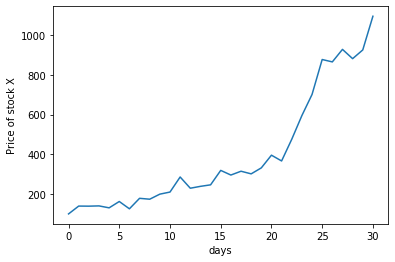
\includegraphics{figures/lesson6_solutions_5_0.png}
\end{center}
\end{Answer}

%\clearpage
%\chapter{Interest Rate Swap and Swaptions}\label{introduction-to-python---lesson-9}

\begin{Exercise}[title={(Swaption Class)}]
  Add to \texttt{finmarkets} module a class to valuate swaptions, it should have as attributes the underlying IRS, the swap rate volatility and the exercise date.
  The class should have the capability of estimating the payoff of the swaptions both with the Black-Scholes formula and Monte Carlo Simulation.
\end{Exercise}

\begin{Answer}
  \begin{tcolorbox}[breakable, size=fbox, boxrule=1pt, pad at break*=1mm,colback=cellbackground, colframe=cellborder]
\begin{Verbatim}[commandchars=\\\{\}]
\PY{k}{class} \PY{n+nc}{InterestRateSwaption}\PY{p}{:}
    
    \PY{k}{def} \PY{n+nf}{\PYZus{}\PYZus{}init\PYZus{}\PYZus{}}\PY{p}{(}\PY{n+nb+bp}{self}\PY{p}{,} \PY{n}{exercise\PYZus{}date}\PY{p}{,} \PY{n}{irs}\PY{p}{)}\PY{p}{:}
        \PY{n+nb+bp}{self}\PY{o}{.}\PY{n}{exercise\PYZus{}date} \PY{o}{=} \PY{n}{exercise\PYZus{}date}
        \PY{n+nb+bp}{self}\PY{o}{.}\PY{n}{irs} \PY{o}{=} \PY{n}{irs}
        
    \PY{k}{def} \PY{n+nf}{npv\PYZus{}bs}\PY{p}{(}\PY{n+nb+bp}{self}\PY{p}{,} \PY{n}{discount\PYZus{}curve}\PY{p}{,} \PY{n}{libor\PYZus{}curve}\PY{p}{,} \PY{n}{sigma}\PY{p}{)}\PY{p}{:}
        
        \PY{n}{A} \PY{o}{=} \PY{n+nb+bp}{self}\PY{o}{.}\PY{n}{irs}\PY{o}{.}\PY{n}{annuity}\PY{p}{(}\PY{n}{discount\PYZus{}curve}\PY{p}{)}
        \PY{n}{S} \PY{o}{=} \PY{n+nb+bp}{self}\PY{o}{.}\PY{n}{irs}\PY{o}{.}\PY{n}{swap\PYZus{}rate}\PY{p}{(}\PY{n}{discount\PYZus{}curve}\PY{p}{,} \PY{n}{libor\PYZus{}curve}\PY{p}{)}

        \PY{n}{T} \PY{o}{=} \PY{p}{(}\PY{n+nb+bp}{self}\PY{o}{.}\PY{n}{exercise\PYZus{}date} \PY{o}{\PYZhy{}} \PY{n}{discount\PYZus{}curve}\PY{o}{.}\PY{n}{today}\PY{p}{)}\PY{o}{.}\PY{n}{days} \PY{o}{/} \PY{l+m+mi}{365}

        \PY{n}{d1} \PY{o}{=} \PY{p}{(}\PY{n}{math}\PY{o}{.}\PY{n}{log}\PY{p}{(}\PY{n}{S}\PY{o}{/}\PY{n+nb+bp}{self}\PY{o}{.}\PY{n}{irs}\PY{o}{.}\PY{n}{fixed\PYZus{}rate}\PY{p}{)} \PY{o}{+} \PY{l+m+mf}{0.5} \PY{o}{*} \PY{n}{sigma}\PY{o}{*}\PY{o}{*}\PY{l+m+mi}{2} \PY{o}{*} \PY{n}{T}\PY{p}{)} \PY{o}{/} \PY{p}{(}\PY{n}{sigma} \PY{o}{*} \PY{n}{T}\PY{o}{*}\PY{o}{*}\PY{l+m+mf}{0.5}\PY{p}{)}
        \PY{n}{d2} \PY{o}{=} \PY{n}{d1} \PY{o}{\PYZhy{}} \PY{p}{(}\PY{n}{sigma} \PY{o}{*} \PY{n}{T}\PY{o}{*}\PY{o}{*}\PY{l+m+mf}{0.5}\PY{p}{)}

        \PY{n}{npv} \PY{o}{=} \PY{n+nb+bp}{self}\PY{o}{.}\PY{n}{irs}\PY{o}{.}\PY{n}{notional} \PY{o}{*} \PY{n}{A} \PY{o}{*} \PY{p}{(}\PY{n}{S} \PY{o}{*} \PY{n}{scipy}\PY{o}{.}\PY{n}{stats}\PY{o}{.}\PY{n}{norm}\PY{o}{.}\PY{n}{cdf}\PY{p}{(}\PY{n}{d1}\PY{p}{)} \PY{o}{\PYZhy{}} 
                                       \PY{n+nb+bp}{self}\PY{o}{.}\PY{n}{irs}\PY{o}{.}\PY{n}{fixed\PYZus{}rate} \PY{o}{*} \PY{n}{scipy}\PY{o}{.}\PY{n}{stats}\PY{o}{.}\PY{n}{norm}\PY{o}{.}\PY{n}{cdf}\PY{p}{(}\PY{n}{d2}\PY{p}{)}\PY{p}{)}
        
        \PY{k}{return} \PY{n}{npv}
    
    \PY{k}{def} \PY{n+nf}{npv\PYZus{}mc}\PY{p}{(}\PY{n+nb+bp}{self}\PY{p}{,} \PY{n}{discount\PYZus{}curve}\PY{p}{,} \PY{n}{libor\PYZus{}curve}\PY{p}{,} \PY{n}{sigma}\PY{p}{,} \PY{n}{n\PYZus{}scenarios}\PY{o}{=}\PY{l+m+mi}{10000}\PY{p}{)}\PY{p}{:}
        
        \PY{n}{A} \PY{o}{=} \PY{n+nb+bp}{self}\PY{o}{.}\PY{n}{irs}\PY{o}{.}\PY{n}{annuity}\PY{p}{(}\PY{n}{discount\PYZus{}curve}\PY{p}{)}
        \PY{n}{S} \PY{o}{=} \PY{n+nb+bp}{self}\PY{o}{.}\PY{n}{irs}\PY{o}{.}\PY{n}{swap\PYZus{}rate}\PY{p}{(}\PY{n}{discount\PYZus{}curve}\PY{p}{,} \PY{n}{libor\PYZus{}curve}\PY{p}{)}

        \PY{n}{T} \PY{o}{=} \PY{p}{(}\PY{n+nb+bp}{self}\PY{o}{.}\PY{n}{exercise\PYZus{}date} \PY{o}{\PYZhy{}} \PY{n}{discount\PYZus{}curve}\PY{o}{.}\PY{n}{today}\PY{p}{)}\PY{o}{.}\PY{n}{days} \PY{o}{/} \PY{l+m+mi}{365}
        \PY{n}{discounted\PYZus{}payoffs} \PY{o}{=} \PY{p}{[}\PY{p}{]}

        \PY{k}{for} \PY{n}{i\PYZus{}scenario} \PY{o+ow}{in} \PY{n+nb}{range}\PY{p}{(}\PY{n}{n\PYZus{}scenarios}\PY{p}{)}\PY{p}{:}
            \PY{n}{S\PYZus{}simulated} \PY{o}{=} \PY{n}{S} \PY{o}{*} \PY{n}{math}\PY{o}{.}\PY{n}{exp}\PY{p}{(}\PY{o}{\PYZhy{}}\PY{l+m+mf}{0.5} \PY{o}{*} \PY{n}{sigma} \PY{o}{*} \PY{n}{sigma} \PY{o}{*} \PY{n}{T} \PY{o}{+}
                                       \PY{n}{sigma} \PY{o}{*} \PY{n}{math}\PY{o}{.}\PY{n}{sqrt}\PY{p}{(}\PY{n}{T}\PY{p}{)} \PY{o}{*} \PY{n}{numpy}\PY{o}{.}\PY{n}{random}\PY{o}{.}\PY{n}{normal}\PY{p}{(}\PY{p}{)}\PY{p}{)}

            \PY{n}{swap\PYZus{}npv} \PY{o}{=} \PY{n+nb+bp}{self}\PY{o}{.}\PY{n}{irs}\PY{o}{.}\PY{n}{notional} \PY{o}{*} \PY{p}{(}\PY{n}{S\PYZus{}simulated} \PY{o}{\PYZhy{}} \PY{n+nb+bp}{self}\PY{o}{.}\PY{n}{irs}\PY{o}{.}\PY{n}{fixed\PYZus{}rate}\PY{p}{)} \PY{o}{*} \PY{n}{A}
            \PY{n}{discounted\PYZus{}payoffs}\PY{o}{.}\PY{n}{append}\PY{p}{(}\PY{n+nb}{max}\PY{p}{(}\PY{l+m+mi}{0}\PY{p}{,} \PY{n}{swap\PYZus{}npv}\PY{p}{)}\PY{p}{)}

        \PY{n}{npv\PYZus{}mc} \PY{o}{=} \PY{n}{numpy}\PY{o}{.}\PY{n}{mean}\PY{p}{(}\PY{n}{discounted\PYZus{}payoffs}\PY{p}{)}
        \PY{n}{npv\PYZus{}error} \PY{o}{=} \PY{l+m+mi}{3} \PY{o}{*} \PY{n}{numpy}\PY{o}{.}\PY{n}{std}\PY{p}{(}\PY{n}{discounted\PYZus{}payoffs}\PY{p}{)} \PY{o}{/} \PY{n}{math}\PY{o}{.}\PY{n}{sqrt}\PY{p}{(}\PY{n}{n\PYZus{}scenarios}\PY{p}{)}
        
        \PY{k}{return} \PY{n}{npv\PYZus{}mc}\PY{p}{,} \PY{n}{npv\PYZus{}error}
\end{Verbatim}
\end{tcolorbox}
\end{Answer}

\begin{Exercise}[title={(Swaption)}]
Suppouse that the LIBOR Forward rates and the discount curve are those defined in \href{https://drive.google.com/file/d/1dm5oZnZKmJM6UrV0L32OcqD5Tzs9SI9A/view?usp=sharing}{libor.xlsx} and \href{https://drive.google.com/file/d/14R22r7m-6VpQ_P79D3qHdK0QN_mOQ_UB/view?usp=sharing}{discount\_curve.xlsx} respectively.
Determine the value of an option to pay a fixed rate of 4\% and receives LIBOR on a 5 year swap starting in 1 year. Assume the notional is 100 EUR, the exercise date is on October, 30th 2020 and the swap rate volatility is 15\%.

\textbf{Hint:} add \texttt{InterestRateSwap} class to \texttt{finmarkets.py}.
\end{Exercise}

\begin{Answer}
\begin{tcolorbox}[size=fbox, boxrule=1pt, colback=cellbackground, colframe=cellborder]
\begin{Verbatim}[commandchars=\\\{\}]
\PY{k+kn}{from} \PY{n+nn}{finmarkets} \PY{k}{import} \PY{n}{InterestRateSwap}
\PY{k+kn}{from} \PY{n+nn}{datetime} \PY{k}{import} \PY{n}{date}
\PY{k+kn}{from} \PY{n+nn}{dateutil}\PY{n+nn}{.}\PY{n+nn}{relativedelta} \PY{k}{import} \PY{n}{relativedelta}
\PY{k+kn}{from} \PY{n+nn}{curve\PYZus{}data} \PY{k}{import} \PY{n}{discount\PYZus{}curve}\PY{p}{,} \PY{n}{libor\PYZus{}curve}
\PY{k+kn}{from} \PY{n+nn}{scipy}\PY{n+nn}{.}\PY{n+nn}{stats} \PY{k}{import} \PY{n}{norm}
\PY{k+kn}{import} \PY{n+nn}{math}

\PY{n}{pricing\PYZus{}date} \PY{o}{=} \PY{n}{date}\PY{o}{.}\PY{n}{today}\PY{p}{(}\PY{p}{)}
\PY{n}{start\PYZus{}date} \PY{o}{=} \PY{n}{date}\PY{o}{.}\PY{n}{today}\PY{p}{(}\PY{p}{)} \PY{o}{+} \PY{n}{relativedelta}\PY{p}{(}\PY{n}{years}\PY{o}{=}\PY{l+m+mi}{1}\PY{p}{)}
\PY{n}{exercise\PYZus{}date} \PY{o}{=} \PY{n}{date}\PY{p}{(}\PY{l+m+mi}{2020}\PY{p}{,} \PY{l+m+mi}{10}\PY{p}{,} \PY{l+m+mi}{30}\PY{p}{)}

\PY{n}{irs} \PY{o}{=} \PY{n}{InterestRateSwap}\PY{p}{(}\PY{n}{start\PYZus{}date}\PY{p}{,} \PY{l+m+mi}{100}\PY{p}{,} \PY{l+m+mf}{0.04}\PY{p}{,} \PY{l+m+mi}{12}\PY{p}{,} \PY{l+m+mi}{5}\PY{p}{)}
\PY{n}{sigma} \PY{o}{=} \PY{l+m+mf}{0.15}

\PY{n}{A} \PY{o}{=} \PY{n}{irs}\PY{o}{.}\PY{n}{annuity}\PY{p}{(}\PY{n}{discount\PYZus{}curve}\PY{p}{)}
\PY{n}{S} \PY{o}{=} \PY{n}{irs}\PY{o}{.}\PY{n}{swap\PYZus{}rate}\PY{p}{(}\PY{n}{discount\PYZus{}curve}\PY{p}{,} \PY{n}{libor\PYZus{}curve}\PY{p}{)}
\PY{n}{T} \PY{o}{=} \PY{p}{(}\PY{n}{exercise\PYZus{}date} \PY{o}{\PYZhy{}} \PY{n}{pricing\PYZus{}date}\PY{p}{)}\PY{o}{.}\PY{n}{days} \PY{o}{/} \PY{l+m+mi}{365}
\PY{n}{d1} \PY{o}{=} \PY{p}{(}\PY{n}{math}\PY{o}{.}\PY{n}{log}\PY{p}{(}\PY{n}{S}\PY{o}{/}\PY{n}{irs}\PY{o}{.}\PY{n}{fixed\PYZus{}rate}\PY{p}{)} \PY{o}{+} \PY{l+m+mf}{0.5} \PY{o}{*} \PY{n}{sigma}\PY{o}{*}\PY{o}{*}\PY{l+m+mi}{2} \PY{o}{*} \PY{n}{T}\PY{p}{)} \PY{o}{/} \PY{p}{(}\PY{n}{sigma} \PY{o}{*} \PY{n}{T}\PY{o}{*}\PY{o}{*}\PY{l+m+mf}{0.5}\PY{p}{)}
\PY{n}{d2} \PY{o}{=} \PY{p}{(}\PY{n}{math}\PY{o}{.}\PY{n}{log}\PY{p}{(}\PY{n}{S}\PY{o}{/}\PY{n}{irs}\PY{o}{.}\PY{n}{fixed\PYZus{}rate}\PY{p}{)} \PY{o}{\PYZhy{}} \PY{l+m+mf}{0.5} \PY{o}{*} \PY{n}{sigma}\PY{o}{*}\PY{o}{*}\PY{l+m+mi}{2} \PY{o}{*} \PY{n}{T}\PY{p}{)} \PY{o}{/} \PY{p}{(}\PY{n}{sigma} \PY{o}{*} \PY{n}{T}\PY{o}{*}\PY{o}{*}\PY{l+m+mf}{0.5}\PY{p}{)}
\PY{n}{npv} \PY{o}{=} \PY{n}{irs}\PY{o}{.}\PY{n}{notional} \PY{o}{*} \PY{n}{A} \PY{o}{*} \PY{p}{(}\PY{n}{S} \PY{o}{*} \PY{n}{norm}\PY{o}{.}\PY{n}{cdf}\PY{p}{(}\PY{n}{d1}\PY{p}{)} \PY{o}{\PYZhy{}} \PY{n}{irs}\PY{o}{.}\PY{n}{fixed\PYZus{}rate} \PY{o}{*} \PY{n}{norm}\PY{o}{.}\PY{n}{cdf}\PY{p}{(}\PY{n}{d2}\PY{p}{)}\PY{p}{)}

\PY{n+nb}{print}\PY{p}{(}\PY{l+s+s2}{\PYZdq{}}\PY{l+s+s2}{Swaption NPV: }\PY{l+s+si}{\PYZob{}:.3f\PYZcb{}}\PY{l+s+s2}{ EUR}\PY{l+s+s2}{\PYZdq{}}\PY{o}{.}\PY{n}{format}\PY{p}{(}\PY{n}{npv}\PY{p}{)}\PY{p}{)}

Swaption NPV: 13.587 EUR

\end{Verbatim}
\end{tcolorbox}
\end{Answer}

%\clearpage
%\chapter{Interest Rate Swap and Swaptions}\label{introduction-to-python---lesson-9}

\begin{Exercise}[title={(Swaption Class)}]
  Add to \texttt{finmarkets} module a class to valuate swaptions, it should have as attributes the underlying IRS, the swap rate volatility and the exercise date.
  The class should have the capability of estimating the payoff of the swaptions both with the Black-Scholes formula and Monte Carlo Simulation.
\end{Exercise}

\begin{Answer}
\begin{tcolorbox}[size=fbox, boxrule=1pt, colback=cellbackground, colframe=cellborder]
\begin{Verbatim}[commandchars=\\\{\}]
\PY{k}{class} \PY{n+nc}{InterestRateSwaption}\PY{p}{:}    
    \PY{k}{def} \PY{n+nf}{\PYZus{}\PYZus{}init\PYZus{}\PYZus{}}\PY{p}{(}\PY{n+nb+bp}{self}\PY{p}{,} \PY{n}{exercise\PYZus{}date}\PY{p}{,} \PY{n}{irs}\PY{p}{)}\PY{p}{:}
        \PY{n+nb+bp}{self}\PY{o}{.}\PY{n}{exercise\PYZus{}date} \PY{o}{=} \PY{n}{exercise\PYZus{}date}
        \PY{n+nb+bp}{self}\PY{o}{.}\PY{n}{irs} \PY{o}{=} \PY{n}{irs}
        
    \PY{k}{def} \PY{n+nf}{npv\PYZus{}bs}\PY{p}{(}\PY{n+nb+bp}{self}\PY{p}{,} \PY{n}{discount\PYZus{}curve}\PY{p}{,} \PY{n}{libor\PYZus{}curve}\PY{p}{,} \PY{n}{sigma}\PY{p}{)}\PY{p}{:}
        \PY{n}{A} \PY{o}{=} \PY{n+nb+bp}{self}\PY{o}{.}\PY{n}{irs}\PY{o}{.}\PY{n}{annuity}\PY{p}{(}\PY{n}{discount\PYZus{}curve}\PY{p}{)}
        \PY{n}{S} \PY{o}{=} \PY{n+nb+bp}{self}\PY{o}{.}\PY{n}{irs}\PY{o}{.}\PY{n}{swap\PYZus{}rate}\PY{p}{(}\PY{n}{discount\PYZus{}curve}\PY{p}{,} \PY{n}{libor\PYZus{}curve}\PY{p}{)}
        \PY{n}{T} \PY{o}{=} \PY{p}{(}\PY{n+nb+bp}{self}\PY{o}{.}\PY{n}{exercise\PYZus{}date} \PY{o}{\PYZhy{}} \PY{n}{discount\PYZus{}curve}\PY{o}{.}\PY{n}{today}\PY{p}{)}\PY{o}{.}\PY{n}{days} \PY{o}{/} \PY{l+m+mi}{365}
        \PY{n}{d1} \PY{o}{=} \PY{p}{(}\PY{n}{math}\PY{o}{.}\PY{n}{log}\PY{p}{(}\PY{n}{S}\PY{o}{/}\PY{n+nb+bp}{self}\PY{o}{.}\PY{n}{irs}\PY{o}{.}\PY{n}{fixed\PYZus{}rate}\PY{p}{)} \PY{o}{+} \PY{l+m+mf}{0.5} \PY{o}{*} \PY{n}{sigma}\PY{o}{*}\PY{o}{*}\PY{l+m+mi}{2} \PY{o}{*} \PY{n}{T}\PY{p}{)} 
             \PY{o}{/} \PY{p}{(}\PY{n}{sigma} \PY{o}{*} \PY{n}{T}\PY{o}{*}\PY{o}{*}\PY{l+m+mf}{0.5}\PY{p}{)}
        \PY{n}{d2} \PY{o}{=} \PY{n}{d1} \PY{o}{\PYZhy{}} \PY{p}{(}\PY{n}{sigma} \PY{o}{*} \PY{n}{T}\PY{o}{*}\PY{o}{*}\PY{l+m+mf}{0.5}\PY{p}{)}
        \PY{n}{npv} \PY{o}{=} \PY{n+nb+bp}{self}\PY{o}{.}\PY{n}{irs}\PY{o}{.}\PY{n}{notional} \PY{o}{*} \PY{n}{A} \PY{o}{*} \PY{p}{(}\PY{n}{S} \PY{o}{*} \PY{n}{scipy}\PY{o}{.}\PY{n}{stats}\PY{o}{.}\PY{n}{norm}\PY{o}{.}\PY{n}{cdf}\PY{p}{(}\PY{n}{d1}\PY{p}{)} \PY{o}{\PYZhy{}} 
              \PY{n+nb+bp}{self}\PY{o}{.}\PY{n}{irs}\PY{o}{.}\PY{n}{fixed\PYZus{}rate} \PY{o}{*} \PY{n}{scipy}\PY{o}{.}\PY{n}{stats}\PY{o}{.}\PY{n}{norm}\PY{o}{.}\PY{n}{cdf}\PY{p}{(}\PY{n}{d2}\PY{p}{)}\PY{p}{)}
        \PY{k}{return} \PY{n}{npv}
\end{Verbatim}
\end{tcolorbox}
\begin{tcolorbox}[size=fbox, boxrule=1pt, colback=cellbackground, colframe=cellborder]
\begin{Verbatim}[commandchars=\\\{\}]
    
    \PY{k}{def} \PY{n+nf}{npv\PYZus{}mc}\PY{p}{(}\PY{n+nb+bp}{self}\PY{p}{,} \PY{n}{discount\PYZus{}curve}\PY{p}{,} \PY{n}{libor\PYZus{}curve}\PY{p}{,} \PY{n}{sigma}\PY{p}{,} \PY{n}{n\PYZus{}scenarios}\PY{o}{=}\PY{l+m+mi}{10000}\PY{p}{)}\PY{p}{:}
        \PY{n}{A} \PY{o}{=} \PY{n+nb+bp}{self}\PY{o}{.}\PY{n}{irs}\PY{o}{.}\PY{n}{annuity}\PY{p}{(}\PY{n}{discount\PYZus{}curve}\PY{p}{)}
        \PY{n}{S} \PY{o}{=} \PY{n+nb+bp}{self}\PY{o}{.}\PY{n}{irs}\PY{o}{.}\PY{n}{swap\PYZus{}rate}\PY{p}{(}\PY{n}{discount\PYZus{}curve}\PY{p}{,} \PY{n}{libor\PYZus{}curve}\PY{p}{)}
        \PY{n}{T} \PY{o}{=} \PY{p}{(}\PY{n+nb+bp}{self}\PY{o}{.}\PY{n}{exercise\PYZus{}date} \PY{o}{\PYZhy{}} \PY{n}{discount\PYZus{}curve}\PY{o}{.}\PY{n}{today}\PY{p}{)}\PY{o}{.}\PY{n}{days} \PY{o}{/} \PY{l+m+mi}{365}
        \PY{n}{discounted\PYZus{}payoffs} \PY{o}{=} \PY{p}{[}\PY{p}{]}
        \PY{k}{for} \PY{n}{i\PYZus{}scenario} \PY{o+ow}{in} \PY{n+nb}{range}\PY{p}{(}\PY{n}{n\PYZus{}scenarios}\PY{p}{)}\PY{p}{:}
            \PY{n}{S\PYZus{}simulated} \PY{o}{=} \PY{n}{S} \PY{o}{*} \PY{n}{math}\PY{o}{.}\PY{n}{exp}\PY{p}{(}\PY{o}{\PYZhy{}}\PY{l+m+mf}{0.5} \PY{o}{*} \PY{n}{sigma} \PY{o}{*} \PY{n}{sigma} \PY{o}{*} \PY{n}{T} \PY{o}{+}
                          \PY{n}{sigma} \PY{o}{*} \PY{n}{math}\PY{o}{.}\PY{n}{sqrt}\PY{p}{(}\PY{n}{T}\PY{p}{)} \PY{o}{*} \PY{n}{numpy}\PY{o}{.}\PY{n}{random}\PY{o}{.}\PY{n}{normal}\PY{p}{(}\PY{p}{)}\PY{p}{)}
            \PY{n}{swap\PYZus{}npv} \PY{o}{=} \PY{n+nb+bp}{self}\PY{o}{.}\PY{n}{irs}\PY{o}{.}\PY{n}{notional} \PY{o}{*} \PY{p}{(}\PY{n}{S\PYZus{}simulated} \PY{o}{\PYZhy{}} \PY{n+nb+bp}{self}\PY{o}{.}\PY{n}{irs}\PY{o}{.}\PY{n}{fixed\PYZus{}rate}\PY{p}{)} \PY{o}{*} \PY{n}{A}
            \PY{n}{discounted\PYZus{}payoffs}\PY{o}{.}\PY{n}{append}\PY{p}{(}\PY{n+nb}{max}\PY{p}{(}\PY{l+m+mi}{0}\PY{p}{,} \PY{n}{swap\PYZus{}npv}\PY{p}{)}\PY{p}{)}
        \PY{n}{npv\PYZus{}mc} \PY{o}{=} \PY{n}{numpy}\PY{o}{.}\PY{n}{mean}\PY{p}{(}\PY{n}{discounted\PYZus{}payoffs}\PY{p}{)}
        \PY{n}{npv\PYZus{}error} \PY{o}{=} \PY{l+m+mi}{3} \PY{o}{*} \PY{n}{numpy}\PY{o}{.}\PY{n}{std}\PY{p}{(}\PY{n}{discounted\PYZus{}payoffs}\PY{p}{)} \PY{o}{/} \PY{n}{math}\PY{o}{.}\PY{n}{sqrt}\PY{p}{(}\PY{n}{n\PYZus{}scenarios}\PY{p}{)}
        
        \PY{k}{return} \PY{n}{npv\PYZus{}mc}\PY{p}{,} \PY{n}{npv\PYZus{}error}
\end{Verbatim}
\end{tcolorbox}
\end{Answer}

\begin{Exercise}[title={(Swaption)}]
Suppouse that the LIBOR Forward rates and the discount curve are those defined in \href{https://drive.google.com/file/d/1dm5oZnZKmJM6UrV0L32OcqD5Tzs9SI9A/view?usp=sharing}{libor.xlsx} and \href{https://drive.google.com/file/d/14R22r7m-6VpQ_P79D3qHdK0QN_mOQ_UB/view?usp=sharing}{discount\_curve.xlsx} respectively.
Determine the value of an option to pay a fixed rate of 4\% and receives LIBOR on a 5 year swap starting in 1 year. Assume the notional is 100 EUR, the exercise date is on October, 30th 2020 and the swap rate volatility is 15\%.

\textbf{Hint:} add \texttt{InterestRateSwap} class to \texttt{finmarkets.py}.
\end{Exercise}

\begin{Answer}
\begin{tcolorbox}[size=fbox, boxrule=1pt, colback=cellbackground, colframe=cellborder]
\begin{Verbatim}[commandchars=\\\{\}]
\PY{k+kn}{from} \PY{n+nn}{finmarkets} \PY{k}{import} \PY{n}{InterestRateSwap}
\PY{k+kn}{from} \PY{n+nn}{datetime} \PY{k}{import} \PY{n}{date}
\PY{k+kn}{from} \PY{n+nn}{dateutil}\PY{n+nn}{.}\PY{n+nn}{relativedelta} \PY{k}{import} \PY{n}{relativedelta}
\PY{k+kn}{from} \PY{n+nn}{curve\PYZus{}data} \PY{k}{import} \PY{n}{discount\PYZus{}curve}\PY{p}{,} \PY{n}{libor\PYZus{}curve}
\PY{k+kn}{from} \PY{n+nn}{scipy}\PY{n+nn}{.}\PY{n+nn}{stats} \PY{k}{import} \PY{n}{norm}
\PY{k+kn}{import} \PY{n+nn}{math}

\PY{n}{pricing\PYZus{}date} \PY{o}{=} \PY{n}{date}\PY{o}{.}\PY{n}{today}\PY{p}{(}\PY{p}{)}
\PY{n}{start\PYZus{}date} \PY{o}{=} \PY{n}{date}\PY{o}{.}\PY{n}{today}\PY{p}{(}\PY{p}{)} \PY{o}{+} \PY{n}{relativedelta}\PY{p}{(}\PY{n}{years}\PY{o}{=}\PY{l+m+mi}{1}\PY{p}{)}
\PY{n}{exercise\PYZus{}date} \PY{o}{=} \PY{n}{date}\PY{p}{(}\PY{l+m+mi}{2020}\PY{p}{,} \PY{l+m+mi}{10}\PY{p}{,} \PY{l+m+mi}{30}\PY{p}{)}
\end{Verbatim}
\end{tcolorbox}

\begin{tcolorbox}[size=fbox, boxrule=1pt, colback=cellbackground, colframe=cellborder]
\begin{Verbatim}[commandchars=\\\{\}]
\PY{n}{irs} \PY{o}{=} \PY{n}{InterestRateSwap}\PY{p}{(}\PY{n}{start\PYZus{}date}\PY{p}{,} \PY{l+m+mi}{100}\PY{p}{,} \PY{l+m+mf}{0.04}\PY{p}{,} \PY{l+m+mi}{12}\PY{p}{,} \PY{l+m+mi}{5}\PY{p}{)}
\PY{n}{sigma} \PY{o}{=} \PY{l+m+mf}{0.15}

\PY{n}{A} \PY{o}{=} \PY{n}{irs}\PY{o}{.}\PY{n}{annuity}\PY{p}{(}\PY{n}{discount\PYZus{}curve}\PY{p}{)}
\PY{n}{S} \PY{o}{=} \PY{n}{irs}\PY{o}{.}\PY{n}{swap\PYZus{}rate}\PY{p}{(}\PY{n}{discount\PYZus{}curve}\PY{p}{,} \PY{n}{libor\PYZus{}curve}\PY{p}{)}
\PY{n}{T} \PY{o}{=} \PY{p}{(}\PY{n}{exercise\PYZus{}date} \PY{o}{\PYZhy{}} \PY{n}{pricing\PYZus{}date}\PY{p}{)}\PY{o}{.}\PY{n}{days} \PY{o}{/} \PY{l+m+mi}{365}
\PY{n}{d1} \PY{o}{=} \PY{p}{(}\PY{n}{math}\PY{o}{.}\PY{n}{log}\PY{p}{(}\PY{n}{S}\PY{o}{/}\PY{n}{irs}\PY{o}{.}\PY{n}{fixed\PYZus{}rate}\PY{p}{)} \PY{o}{+} \PY{l+m+mf}{0.5} \PY{o}{*} \PY{n}{sigma}\PY{o}{*}\PY{o}{*}\PY{l+m+mi}{2} \PY{o}{*} \PY{n}{T}\PY{p}{)} \PY{o}{/} \PY{p}{(}\PY{n}{sigma} \PY{o}{*} \PY{n}{T}\PY{o}{*}\PY{o}{*}\PY{l+m+mf}{0.5}\PY{p}{)}
\PY{n}{d2} \PY{o}{=} \PY{p}{(}\PY{n}{math}\PY{o}{.}\PY{n}{log}\PY{p}{(}\PY{n}{S}\PY{o}{/}\PY{n}{irs}\PY{o}{.}\PY{n}{fixed\PYZus{}rate}\PY{p}{)} \PY{o}{\PYZhy{}} \PY{l+m+mf}{0.5} \PY{o}{*} \PY{n}{sigma}\PY{o}{*}\PY{o}{*}\PY{l+m+mi}{2} \PY{o}{*} \PY{n}{T}\PY{p}{)} \PY{o}{/} \PY{p}{(}\PY{n}{sigma} \PY{o}{*} \PY{n}{T}\PY{o}{*}\PY{o}{*}\PY{l+m+mf}{0.5}\PY{p}{)}
\PY{n}{npv} \PY{o}{=} \PY{n}{irs}\PY{o}{.}\PY{n}{notional} \PY{o}{*} \PY{n}{A} \PY{o}{*} \PY{p}{(}\PY{n}{S} \PY{o}{*} \PY{n}{norm}\PY{o}{.}\PY{n}{cdf}\PY{p}{(}\PY{n}{d1}\PY{p}{)} \PY{o}{\PYZhy{}} \PY{n}{irs}\PY{o}{.}\PY{n}{fixed\PYZus{}rate} \PY{o}{*} \PY{n}{norm}\PY{o}{.}\PY{n}{cdf}\PY{p}{(}\PY{n}{d2}\PY{p}{)}\PY{p}{)}

\PY{n+nb}{print}\PY{p}{(}\PY{l+s+s2}{\PYZdq{}}\PY{l+s+s2}{Swaption NPV: }\PY{l+s+si}{\PYZob{}:.3f\PYZcb{}}\PY{l+s+s2}{ EUR}\PY{l+s+s2}{\PYZdq{}}\PY{o}{.}\PY{n}{format}\PY{p}{(}\PY{n}{npv}\PY{p}{)}\PY{p}{)}

Swaption NPV: 13.587 EUR
\end{Verbatim}
\end{tcolorbox}
\end{Answer}

%\clearpage
%\chapter{Copulas and its Applications}\label{introduction-to-python---lesson-11}

\begin{Exercise}[title={(Distribution Transformation)}]
	Using the \emph{probability integral transform} transform a Gumbel distribution into a Gaussian. Plot also all the distributions involved in the transformation.
\end{Exercise}

\begin{Answer}
\begin{tcolorbox}[size=fbox, boxrule=1pt, colback=cellbackground, colframe=cellborder]
\begin{Verbatim}[commandchars=\\\{\}]
\PY{k+kn}{from} \PY{n+nn}{scipy}\PY{n+nn}{.}\PY{n+nn}{stats} \PY{k}{import} \PY{n}{gumbel\PYZus{}l}\PY{p}{,} \PY{n}{norm}
	
\PY{n}{gumbel} \PY{o}{=} \PY{n}{gumbel\PYZus{}l}\PY{p}{(}\PY{p}{)}
\PY{n}{xg} \PY{o}{=} \PY{n}{gumbel}\PY{o}{.}\PY{n}{rvs}\PY{p}{(}\PY{l+m+mi}{100000}\PY{p}{)}
\PY{n}{xu} \PY{o}{=} \PY{n}{gumbel}\PY{o}{.}\PY{n}{cdf}\PY{p}{(}\PY{n}{xg}\PY{p}{)}
\PY{n}{xn} \PY{o}{=} \PY{n}{norm}\PY{o}{.}\PY{n}{ppf}\PY{p}{(}\PY{n}{xu}\PY{p}{)}

\PY{k+kn}{from} \PY{n+nn}{matplotlib} \PY{k}{import} \PY{n}{pyplot} \PY{k}{as} \PY{n}{plt}

\PY{n}{sub1} \PY{o}{=} \PY{n}{plt}\PY{o}{.}\PY{n}{subplot}\PY{p}{(}\PY{l+m+mi}{1}\PY{p}{,} \PY{l+m+mi}{3}\PY{p}{,} \PY{l+m+mi}{1}\PY{p}{)}
\PY{n}{sub1}\PY{o}{.}\PY{n}{hist}\PY{p}{(}\PY{n}{xg}\PY{p}{,} \PY{l+m+mi}{50}\PY{p}{)}
\PY{n}{sub1}\PY{o}{.}\PY{n}{grid}\PY{p}{(}\PY{k+kc}{True}\PY{p}{)}
\PY{n}{sub1}\PY{o}{.}\PY{n}{set\PYZus{}xlabel}\PY{p}{(}\PY{l+s+s2}{\PYZdq{}}\PY{l+s+s2}{\PYZdl{}x\PYZus{}}\PY{l+s+si}{\PYZob{}gumbel\PYZcb{}}\PY{l+s+s2}{\PYZdl{}}\PY{l+s+s2}{\PYZdq{}}\PY{p}{)}

\PY{n}{sub2} \PY{o}{=} \PY{n}{plt}\PY{o}{.}\PY{n}{subplot}\PY{p}{(}\PY{l+m+mi}{1}\PY{p}{,} \PY{l+m+mi}{3}\PY{p}{,} \PY{l+m+mi}{2}\PY{p}{)}
\PY{n}{sub2}\PY{o}{.}\PY{n}{hist}\PY{p}{(}\PY{n}{xu}\PY{p}{,} \PY{l+m+mi}{50}\PY{p}{)}
\PY{n}{sub2}\PY{o}{.}\PY{n}{grid}\PY{p}{(}\PY{k+kc}{True}\PY{p}{)}
\PY{n}{sub2}\PY{o}{.}\PY{n}{set\PYZus{}xlabel}\PY{p}{(}\PY{l+s+s2}{\PYZdq{}}\PY{l+s+s2}{\PYZdl{}x\PYZus{}}\PY{l+s+si}{\PYZob{}uniform\PYZcb{}}\PY{l+s+s2}{\PYZdl{}}\PY{l+s+s2}{\PYZdq{}}\PY{p}{)}

\PY{n}{sub3} \PY{o}{=} \PY{n}{plt}\PY{o}{.}\PY{n}{subplot}\PY{p}{(}\PY{l+m+mi}{1}\PY{p}{,} \PY{l+m+mi}{3}\PY{p}{,} \PY{l+m+mi}{3}\PY{p}{)}
\PY{n}{sub3}\PY{o}{.}\PY{n}{hist}\PY{p}{(}\PY{n}{xn}\PY{p}{,} \PY{l+m+mi}{50}\PY{p}{)}
\PY{n}{sub3}\PY{o}{.}\PY{n}{grid}\PY{p}{(}\PY{k+kc}{True}\PY{p}{)}
\PY{n}{sub3}\PY{o}{.}\PY{n}{set\PYZus{}xlabel}\PY{p}{(}\PY{l+s+s2}{\PYZdq{}}\PY{l+s+s2}{\PYZdl{}x\PYZus{}}\PY{l+s+si}{\PYZob{}normal\PYZcb{}}\PY{l+s+s2}{\PYZdl{}}\PY{l+s+s2}{\PYZdq{}}\PY{p}{)}
	
\PY{n}{plt}\PY{o}{.}\PY{n}{show}\PY{p}{(}\PY{p}{)}
\end{Verbatim}
\end{tcolorbox}

\begin{center}
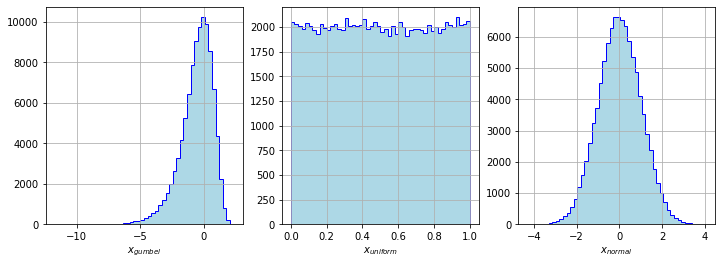
\includegraphics{figures/ex_gumbel_to_gauss.png}
\end{center}
\end{Answer}

\begin{Exercise}[title={(Random Numbers)}]
Without using the corresponding \texttt{rvs()} method try to generate 10 random numbers distributed as Beta distribution (parameters \texttt{a=3} and \texttt{b=10}).

\textbf{Hint:} starts with generating uniformly distributed random numbers.
\end{Exercise}	

\begin{Answer}
\begin{tcolorbox}[size=fbox, boxrule=1pt, colback=cellbackground, colframe=cellborder]
\begin{Verbatim}[commandchars=\\\{\}]
\PY{k+kn}{from} \PY{n+nn}{scipy}\PY{n+nn}{.}\PY{n+nn}{stats} \PY{k}{import} \PY{n}{beta}\PY{p}{,} \PY{n}{uniform}
		
\PY{n}{x} \PY{o}{=} \PY{n}{uniform}\PY{o}{.}\PY{n}{rvs}\PY{p}{(}\PY{n}{size}\PY{o}{=}\PY{l+m+mi}{10}\PY{p}{)}
\PY{n}{b} \PY{o}{=} \PY{n}{beta}\PY{p}{(}\PY{n}{a}\PY{o}{=}\PY{l+m+mi}{3}\PY{p}{,} \PY{n}{b}\PY{o}{=}\PY{l+m+mi}{10}\PY{p}{)}
\PY{n}{x\PYZus{}b} \PY{o}{=} \PY{n}{b}\PY{o}{.}\PY{n}{ppf}\PY{p}{(}\PY{n}{x}\PY{p}{)}
		
\PY{n+nb}{print} \PY{p}{(}\PY{n}{x\PYZus{}b}\PY{p}{)}

[0.29190237 0.45669406 0.10336582 0.5403107  0.08305872 0.32425694
0.43902811 0.11820592 0.28659784 0.22316621]
\end{Verbatim}
\end{tcolorbox}
\end{Answer}

\begin{Exercise}[title={(Copula)}]
Consider two companies whose default probabilities as a function of time are modeled according to a lognormal distribution with $\sigma =0.5$ (\texttt{scipy.stats.lognorm(0.5)}). Compare the joint 2D distributions in case of no correlation and with a Gaussian correlation of 0.8.

\textbf{Hint:} to plot the joint distribution use \texttt{matplotlib} function \texttt{hist2d(x1, x2, range=[[x1min, x1max], [xmin, x2max]], bins=(50, 50)) }.
\end{Exercise}

\begin{Answer}
\begin{tcolorbox}[size=fbox, boxrule=1pt, colback=cellbackground, colframe=cellborder]
\begin{Verbatim}[commandchars=\\\{\}]
\PY{k+kn}{from} \PY{n+nn}{scipy}\PY{n+nn}{.}\PY{n+nn}{stats} \PY{k}{import} \PY{n}{lognorm}\PY{p}{,} \PY{n}{multivariate\PYZus{}normal}\PY{p}{,} \PY{n}{norm}
\PY{k+kn}{import} \PY{n+nn}{numpy}
		
\PY{n}{numpy}\PY{o}{.}\PY{n}{random}\PY{o}{.}\PY{n}{seed}\PY{p}{(}\PY{l+m+mi}{1}\PY{p}{)}
\PY{n}{samples} \PY{o}{=} \PY{l+m+mi}{1000000}
\PY{n}{l1\PYZus{}uncorr} \PY{o}{=} \PY{n}{lognorm}\PY{p}{(}\PY{l+m+mf}{0.5}\PY{p}{)}\PY{o}{.}\PY{n}{rvs}\PY{p}{(}\PY{n}{size}\PY{o}{=}\PY{n}{samples}\PY{p}{)}
\PY{n}{l2\PYZus{}uncorr} \PY{o}{=} \PY{n}{lognorm}\PY{p}{(}\PY{l+m+mf}{0.5}\PY{p}{)}\PY{o}{.}\PY{n}{rvs}\PY{p}{(}\PY{n}{size}\PY{o}{=}\PY{n}{samples}\PY{p}{)}
\PY{n}{mvnorm} \PY{o}{=} \PY{n}{multivariate\PYZus{}normal}\PY{p}{(}\PY{n}{mean} \PY{o}{=} \PY{p}{(}\PY{l+m+mi}{0}\PY{p}{,} \PY{l+m+mi}{0}\PY{p}{)}\PY{p}{,} \PY{n}{cov}\PY{o}{=}\PY{p}{[}\PY{p}{[}\PY{l+m+mi}{1}\PY{p}{,} \PY{l+m+mf}{0.8}\PY{p}{]}\PY{p}{,}
\PY{p}{[}\PY{l+m+mf}{0.8}\PY{p}{,} \PY{l+m+mi}{1}\PY{p}{]}\PY{p}{]}\PY{p}{)}
\PY{n}{x} \PY{o}{=} \PY{n}{mvnorm}\PY{o}{.}\PY{n}{rvs}\PY{p}{(}\PY{n}{size}\PY{o}{=}\PY{n}{samples}\PY{p}{)}
\PY{n}{x\PYZus{}corr} \PY{o}{=} \PY{n}{norm}\PY{o}{.}\PY{n}{cdf}\PY{p}{(}\PY{n}{x}\PY{p}{)}
\PY{n}{l1\PYZus{}corr} \PY{o}{=} \PY{n}{lognorm}\PY{p}{(}\PY{l+m+mf}{0.5}\PY{p}{)}\PY{o}{.}\PY{n}{ppf}\PY{p}{(}\PY{n}{x\PYZus{}corr}\PY{p}{[}\PY{p}{:}\PY{p}{,} \PY{l+m+mi}{0}\PY{p}{]}\PY{p}{)}
\PY{n}{l2\PYZus{}corr} \PY{o}{=} \PY{n}{lognorm}\PY{p}{(}\PY{l+m+mf}{0.5}\PY{p}{)}\PY{o}{.}\PY{n}{ppf}\PY{p}{(}\PY{n}{x\PYZus{}corr}\PY{p}{[}\PY{p}{:}\PY{p}{,} \PY{l+m+mi}{1}\PY{p}{]}\PY{p}{)}
		
\PY{n}{plt}\PY{o}{.}\PY{n}{figure}\PY{p}{(}\PY{n}{figsize}\PY{o}{=}\PY{p}{(}\PY{l+m+mi}{12}\PY{p}{,} \PY{l+m+mi}{4}\PY{p}{)}\PY{p}{)}
\PY{n}{sub1} \PY{o}{=} \PY{n}{plt}\PY{o}{.}\PY{n}{subplot}\PY{p}{(}\PY{l+m+mi}{1}\PY{p}{,} \PY{l+m+mi}{2}\PY{p}{,} \PY{l+m+mi}{1}\PY{p}{)}
\PY{n}{sub1}\PY{o}{.}\PY{n}{hist2d}\PY{p}{(}\PY{n}{l1\PYZus{}uncorr}\PY{p}{,} \PY{n}{l2\PYZus{}uncorr}\PY{p}{,} \PY{n+nb}{range}\PY{o}{=}\PY{p}{[}\PY{p}{[}\PY{l+m+mi}{0}\PY{p}{,} \PY{l+m+mi}{2}\PY{p}{]}\PY{p}{,} \PY{p}{[}\PY{l+m+mi}{0}\PY{p}{,} \PY{l+m+mi}{2}\PY{p}{]}\PY{p}{]}\PY{p}{,} \PY{n}{bins}\PY{o}{=}\PY{p}{(}\PY{l+m+mi}{100}\PY{p}{,} \PY{l+m+mi}{100}\PY{p}{)}\PY{p}{)}
		
\PY{n}{sub2} \PY{o}{=} \PY{n}{plt}\PY{o}{.}\PY{n}{subplot}\PY{p}{(}\PY{l+m+mi}{1}\PY{p}{,} \PY{l+m+mi}{2}\PY{p}{,} \PY{l+m+mi}{2}\PY{p}{)}
\PY{n}{sub2}\PY{o}{.}\PY{n}{hist2d}\PY{p}{(}\PY{n}{l1\PYZus{}corr}\PY{p}{,} \PY{n}{l2\PYZus{}corr}\PY{p}{,} \PY{n+nb}{range}\PY{o}{=}\PY{p}{[}\PY{p}{[}\PY{l+m+mi}{0}\PY{p}{,} \PY{l+m+mi}{2}\PY{p}{]}\PY{p}{,} \PY{p}{[}\PY{l+m+mi}{0}\PY{p}{,} \PY{l+m+mi}{2}\PY{p}{]}\PY{p}{]}\PY{p}{,} \PY{n}{bins}\PY{o}{=}\PY{p}{(}\PY{l+m+mi}{100}\PY{p}{,} \PY{l+m+mi}{100}\PY{p}{)}\PY{p}{)}
\PY{n}{plt}\PY{o}{.}\PY{n}{show}\PY{p}{(}\PY{p}{)}
\end{Verbatim}
\end{tcolorbox}

\begin{center}
	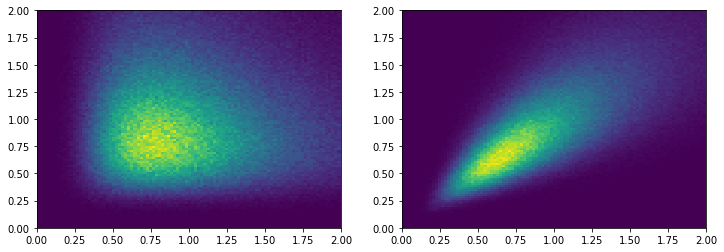
\includegraphics{figures/copula_lognormal.png}
\end{center}

In order to quantify the difference shown with the comparison of the two 2D plots we can calculate the probability that both companies default in the next six months.

So the probability that a single company default in six months regardless the other can be calculated from the \texttt{cdf} of the lognormal distribution.
Hence in case of independent probabilities what required is just the squared of this value
(about 0.07\%).
\begin{tcolorbox}[size=fbox, boxrule=1pt, colback=cellbackground, colframe=cellborder]
\begin{Verbatim}[commandchars=\\\{\}]
\PY{n}{default\PYZus{}6m} \PY{o}{=} \PY{n}{lognorm}\PY{p}{(}\PY{l+m+mf}{0.5}\PY{p}{)}\PY{o}{.}\PY{n}{cdf}\PY{p}{(}\PY{o}{.}\PY{l+m+mi}{5}\PY{p}{)}
\PY{n}{default\PYZus{}6m}\PY{o}{*}\PY{o}{*}\PY{l+m+mi}{2}

0.006860563560014724
\end{Verbatim}
\end{tcolorbox}

In the case of correlation instead we have to loop over the samples from the joint multivariate distribution (with correlation) and check how many times both values are less than \texttt{default\_6m}.

\begin{tcolorbox}[size=fbox, boxrule=1pt, colback=cellbackground, colframe=cellborder]
\begin{Verbatim}[commandchars=\\\{\}]
\PY{n}{success} \PY{o}{=} \PY{l+m+mf}{0.0}
\PY{k}{for} \PY{n}{i} \PY{o+ow}{in} \PY{n+nb}{range}\PY{p}{(}\PY{n}{samples}\PY{p}{)}\PY{p}{:}
    \PY{k}{if} \PY{n+nb}{max}\PY{p}{(}\PY{n}{x\PYZus{}corr}\PY{p}{[}\PY{n}{i}\PY{p}{]}\PY{p}{)} \PY{o}{\PYZlt{}} \PY{n}{default\PYZus{}2}\PY{p}{:}
        \PY{n}{success} \PY{o}{+}\PY{o}{=} \PY{l+m+mi}{1}
		
\PY{n+nb}{print} \PY{p}{(}\PY{n}{success}\PY{o}{/}\PY{n}{samples}\PY{p}{)}

0.044654
\end{Verbatim}
\end{tcolorbox}

This result can be interpreted graphically by saying that the entries in the "square" $[0, 0.5]$ in the left histogram are about 0.7\% of the total while the entries in the right plot in same "square" are about 4.5\% of the total. 
\end{Answer}
%\clearpage
%\chapter{Modeling Correlation between Risks}\label{introduction-to-python---lesson-12}

\begin{Exercise}[title={($n^{th}$ to Default)}]
Estimate the default probabilities for the next 5 years for 6 companies. 
The default correlation between each company is 0.4 and the cumulative probability of default during 
the next 1,2,3,4,5 years is 1\%, 2\%, 5\%, 8\%, 11\% respectively for each company.

When a Gaussian copula is used in order to simulate the defaults determine the 4th-to-default probabilities for each year.
\end{Exercise}
\begin{Answer}
\begin{tcolorbox}[breakable, size=fbox, boxrule=1pt, pad at break*=1mm,colback=cellbackground, colframe=cellborder]
\begin{Verbatim}[commandchars=\\\{\}]
\PY{k+kn}{from} \PY{n+nn}{scipy}\PY{n+nn}{.}\PY{n+nn}{stats} \PY{k}{import} \PY{n}{multivariate\PYZus{}normal}\PY{p}{,} \PY{n}{norm}
	
\PY{n}{p\PYZus{}default} \PY{o}{=} \PY{p}{[}\PY{l+m+mi}{0}\PY{p}{,} \PY{l+m+mf}{0.01}\PY{p}{,} \PY{l+m+mf}{0.02}\PY{p}{,} \PY{l+m+mf}{0.05}\PY{p}{,} \PY{l+m+mf}{0.08}\PY{p}{,} \PY{l+m+mf}{0.11}\PY{p}{]}
	
\PY{n}{mvnorm} \PY{o}{=} \PY{n}{multivariate\PYZus{}normal}\PY{p}{(}\PY{n}{mean}\PY{o}{=}\PY{p}{[}\PY{l+m+mi}{0}\PY{p}{]}\PY{o}{*}\PY{l+m+mi}{6}\PY{p}{,}
\PY{n}{cov} \PY{o}{=} \PY{p}{[}\PY{p}{[}\PY{l+m+mi}{1}\PY{p}{,} \PY{l+m+mf}{0.4}\PY{p}{,} \PY{l+m+mf}{0.4}\PY{p}{,} \PY{l+m+mf}{0.4}\PY{p}{,} \PY{l+m+mf}{0.4}\PY{p}{,} \PY{l+m+mf}{0.4}\PY{p}{]}\PY{p}{,}
       \PY{p}{[}\PY{l+m+mf}{0.4}\PY{p}{,} \PY{l+m+mi}{1}\PY{p}{,} \PY{l+m+mf}{0.4}\PY{p}{,} \PY{l+m+mf}{0.4}\PY{p}{,} \PY{l+m+mf}{0.4}\PY{p}{,} \PY{l+m+mf}{0.4}\PY{p}{]}\PY{p}{,}
       \PY{p}{[}\PY{l+m+mf}{0.4}\PY{p}{,} \PY{l+m+mf}{0.4}\PY{p}{,} \PY{l+m+mi}{1}\PY{p}{,} \PY{l+m+mf}{0.4}\PY{p}{,} \PY{l+m+mf}{0.4}\PY{p}{,} \PY{l+m+mf}{0.4}\PY{p}{]}\PY{p}{,}
       \PY{p}{[}\PY{l+m+mf}{0.4}\PY{p}{,} \PY{l+m+mf}{0.4}\PY{p}{,} \PY{l+m+mf}{0.4}\PY{p}{,} \PY{l+m+mi}{1}\PY{p}{,} \PY{l+m+mf}{0.4}\PY{p}{,} \PY{l+m+mf}{0.4}\PY{p}{]}\PY{p}{,}
       \PY{p}{[}\PY{l+m+mf}{0.4}\PY{p}{,} \PY{l+m+mf}{0.4}\PY{p}{,} \PY{l+m+mf}{0.4}\PY{p}{,} \PY{l+m+mf}{0.4}\PY{p}{,} \PY{l+m+mi}{1}\PY{p}{,} \PY{l+m+mf}{0.4}\PY{p}{]}\PY{p}{,}
       \PY{p}{[}\PY{l+m+mf}{0.4}\PY{p}{,} \PY{l+m+mf}{0.4}\PY{p}{,} \PY{l+m+mf}{0.4}\PY{p}{,} \PY{l+m+mf}{0.4}\PY{p}{,} \PY{l+m+mf}{0.4}\PY{p}{,} \PY{l+m+mi}{1}\PY{p}{]}\PY{p}{]}\PY{p}{)}
	
\PY{n}{n\PYZus{}to\PYZus{}default} \PY{o}{=} \PY{l+m+mi}{4}
\PY{n}{trials} \PY{o}{=} \PY{l+m+mi}{500000}
\PY{n}{result} \PY{o}{=} \PY{p}{[}\PY{l+m+mf}{0.}\PY{p}{,} \PY{l+m+mf}{0.}\PY{p}{,} \PY{l+m+mf}{0.}\PY{p}{,} \PY{l+m+mf}{0.}\PY{p}{,} \PY{l+m+mf}{0.}\PY{p}{,} \PY{l+m+mf}{0.}\PY{p}{]}

\PY{n}{x} \PY{o}{=} \PY{n}{mvnorm}\PY{o}{.}\PY{n}{rvs}\PY{p}{(}\PY{n}{size}\PY{o}{=}\PY{n}{trials}\PY{p}{)}
\end{Verbatim}
\end{tcolorbox}
\begin{tcolorbox}[breakable, size=fbox, boxrule=1pt, pad at break*=1mm,colback=cellbackground, colframe=cellborder]
\begin{Verbatim}[commandchars=\\\{\}]
\PY{k}{for} \PY{n}{n} \PY{o+ow}{in} \PY{n+nb}{range}\PY{p}{(}\PY{n+nb}{len}\PY{p}{(}\PY{n}{x}\PY{p}{)}\PY{p}{)}\PY{p}{:}
    \PY{n}{p} \PY{o}{=} \PY{n+nb}{sorted}\PY{p}{(}\PY{n}{norm}\PY{o}{.}\PY{n}{cdf}\PY{p}{(}\PY{n}{x}\PY{p}{[}\PY{n}{n}\PY{p}{]}\PY{p}{)}\PY{p}{)}
    \PY{k}{for} \PY{n}{i} \PY{o+ow}{in} \PY{n+nb}{range}\PY{p}{(}\PY{l+m+mi}{1}\PY{p}{,} \PY{n+nb}{len}\PY{p}{(}\PY{n}{p\PYZus{}default}\PY{p}{)}\PY{p}{)}\PY{p}{:}
    \PY{k}{if} \PY{n}{p\PYZus{}default}\PY{p}{[}\PY{n}{i}\PY{o}{\PYZhy{}}\PY{l+m+mi}{1}\PY{p}{]} \PY{o}{\PYZlt{}}\PY{o}{=} \PY{n}{p}\PY{p}{[}\PY{n}{n\PYZus{}to\PYZus{}default}\PY{o}{\PYZhy{}}\PY{l+m+mi}{1}\PY{p}{]} \PY{o}{\PYZlt{}}\PY{o}{=} \PY{n}{p\PYZus{}default}\PY{p}{[}\PY{n}{i}\PY{p}{]}\PY{p}{:}
        \PY{n}{result}\PY{p}{[}\PY{n}{i}\PY{p}{]} \PY{o}{+}\PY{o}{=} \PY{l+m+mi}{1}
	
\PY{n+nb}{print} \PY{p}{(}\PY{l+s+s2}{\PYZdq{}}\PY{l+s+s2}{4th\PYZhy{}to\PYZhy{}default probabilies}\PY{l+s+s2}{\PYZdq{}}\PY{p}{)}
	\PY{k}{for} \PY{n}{i} \PY{o+ow}{in} \PY{n+nb}{range}\PY{p}{(}\PY{n+nb}{len}\PY{p}{(}\PY{n}{p\PYZus{}default}\PY{p}{)}\PY{p}{)}\PY{p}{:}
	\PY{n+nb}{print} \PY{p}{(}\PY{l+s+s2}{\PYZdq{}}\PY{l+s+si}{\PYZob{}\PYZcb{}}\PY{l+s+s2}{: }\PY{l+s+si}{\PYZob{}:.4f\PYZcb{}}\PY{l+s+s2}{\PYZdq{}}\PY{o}{.}\PY{n}{format}\PY{p}{(}\PY{n}{i}\PY{p}{,} \PY{n}{result}\PY{p}{[}\PY{n}{i}\PY{p}{]}\PY{o}{/}\PY{n}{trials}\PY{p}{)}\PY{p}{)}

4th-to-default probabilies
0: 0.0000
1: 0.0004
2: 0.0009
3: 0.0059
4: 0.0098
5: 0.0135
\end{Verbatim}
\end{tcolorbox}
\end{Answer}

\begin{Exercise}[title={(Basket Default Swap)}]
Consider a 3-year 5th-to-default basket of ten
reference entities in the situation where the copula correlation is 0.15
and the expected recovery rate, \(R\), is \(40\%\). The term structure
of interest rates is assumed to be flat at 3\%. The default
probabilities for the ten entities are 1\%, 3\% and 7\% respectively.

Determine the breakeven rate and the NPV.
\end{Exercise}
\begin{Answer}	
\begin{tcolorbox}[size=fbox, boxrule=1pt, colback=cellbackground, colframe=cellborder]
\begin{Verbatim}[commandchars=\\\{\}]
\PY{k+kn}{from} \PY{n+nn}{finmarkets\PYZus{}tot} \PY{k}{import} \PY{n}{DiscountCurve}\PY{c+c1}{\PYZsh{}, BasketDefaultSwaps}
\PY{k+kn}{from} \PY{n+nn}{datetime} \PY{k}{import} \PY{n}{date}
\PY{k+kn}{from} \PY{n+nn}{dateutil}\PY{n+nn}{.}\PY{n+nn}{relativedelta} \PY{k}{import} \PY{n}{relativedelta}
	
\PY{n}{n\PYZus{}cds} \PY{o}{=} \PY{l+m+mi}{10}
\PY{n}{rho} \PY{o}{=} \PY{l+m+mf}{0.15}
\PY{n}{l} \PY{o}{=} \PY{l+m+mf}{0.01}
\PY{n}{pillar\PYZus{}dates} \PY{o}{=} \PY{p}{[}\PY{p}{]}
\PY{n}{df} \PY{o}{=} \PY{p}{[}\PY{p}{]}
\PY{n}{observation\PYZus{}date} \PY{o}{=} \PY{n}{date}\PY{o}{.}\PY{n}{today}\PY{p}{(}\PY{p}{)}
\end{Verbatim}
\end{tcolorbox}	

\begin{tcolorbox}[size=fbox, boxrule=1pt, colback=cellbackground, colframe=cellborder]
\begin{Verbatim}[commandchars=\\\{\}]
\PY{k}{for} \PY{n}{i} \PY{o+ow}{in} \PY{n+nb}{range}\PY{p}{(}\PY{l+m+mi}{4}\PY{p}{)}\PY{p}{:}
    \PY{n}{pillar\PYZus{}dates}\PY{o}{.}\PY{n}{append}\PY{p}{(}\PY{n}{observation\PYZus{}date} \PY{o}{+} \PY{n}{relativedelta}\PY{p}{(}\PY{n}{years}\PY{o}{=}\PY{n}{i}\PY{p}{)}\PY{p}{)}
    \PY{n}{df}\PY{o}{.}\PY{n}{append}\PY{p}{(}\PY{l+m+mi}{1}\PY{o}{/}\PY{p}{(}\PY{l+m+mi}{1}\PY{o}{+}\PY{l+m+mf}{0.03}\PY{p}{)}\PY{o}{*}\PY{o}{*}\PY{n}{i}\PY{p}{)}
\PY{n}{dc} \PY{o}{=} \PY{n}{DiscountCurve}\PY{p}{(}\PY{n}{observation\PYZus{}date}\PY{p}{,} \PY{n}{pillar\PYZus{}dates}\PY{p}{,} \PY{n}{df}\PY{p}{)}
	
\PY{n}{Q} \PY{o}{=} \PY{p}{[}\PY{l+m+mf}{0.0}\PY{p}{,} \PY{l+m+mf}{0.01}\PY{p}{,} \PY{l+m+mf}{0.03}\PY{p}{,} \PY{l+m+mf}{0.07}\PY{p}{]}
	
\PY{n}{ndefaults} \PY{o}{=} \PY{l+m+mi}{5}
\PY{n}{basket} \PY{o}{=} \PY{n}{BasketDefaultSwaps}\PY{p}{(}\PY{l+m+mi}{1}\PY{p}{,} \PY{n}{observation\PYZus{}date}\PY{p}{,} \PY{l+m+mf}{0.01}\PY{p}{,} \PY{l+m+mi}{3}\PY{p}{,} \PY{l+m+mi}{12}\PY{p}{,} \PY{n}{n\PYZus{}cds}\PY{p}{,} \PY{n}{rho}\PY{p}{)}
	
\PY{n+nb}{print}\PY{p}{(}\PY{n}{basket}\PY{o}{.}\PY{n}{breakeven}\PY{p}{(}\PY{n}{pillar_dates}\PY{p}{,} \PY{n}{Q}\PY{p}{,} \PY{n}{dc}\PY{p}{,} \PY{n}{ndefaults}\PY{p}{)}\PY{p}{)}
\PY{n+nb}{print}\PY{p}{(}\PY{n}{basket}\PY{o}{.}\PY{n}{npv}\PY{p}{(}\PY{n}{pillar_dates}\PY{p}{,} \PY{n}{Q}\PY{p}{,} \PY{n}{dc}\PY{p}{,} \PY{n}{ndefaults}\PY{p}{)}\PY{p}{)}

0.0002528465216073568
0.11147956240052284
\end{Verbatim}
\end{tcolorbox}	
\end{Answer}

\begin{Exercise}[title={(Cash CDO)}]
Consider a Cash CDO with a maturity of 1 year, made of 125 bonds. 
Each bond pays a coupon of one unit after 1 year and it has not yet defaulted
(the recovery rate $R$ is assumed 0). The CDO has three tranches: equity ([0, 3] defaults), mezzanine ([4, 6] defaults) 
and senior ([7, 125] defaults).

Draw the expected loss as a function of the correlation $\rho$ for the three tranches and 
show that the sum of the losses of each tranche is independent from $\rho$.
\end{Exercise}
\begin{Answer}	
To solve this exercise we need to implement a function that evaluate through the one-factor copula model and the binomial distribution the probability of $l$ defaults.
Then we can compute the expected losses for each tranche and for various values of the correlation parameter $\rho$, saving into a list the results for later plotting.

\begin{tcolorbox}[size=fbox, boxrule=1pt, colback=cellbackground, colframe=cellborder]
\begin{Verbatim}[commandchars=\\\{\}]
\PY{k+kn}{from} \PY{n+nn}{scipy}\PY{n+nn}{.}\PY{n+nn}{stats} \PY{k}{import} \PY{n}{binom}\PY{p}{,} \PY{n}{norm}
\PY{k+kn}{from} \PY{n+nn}{scipy}\PY{n+nn}{.}\PY{n+nn}{integrate} \PY{k}{import} \PY{n}{quad}
\PY{k+kn}{import} \PY{n+nn}{numpy} \PY{k}{as} \PY{n+nn}{np}
			
\PY{n}{N} \PY{o}{=} \PY{l+m+mi}{125}
\PY{n}{A} \PY{o}{=} \PY{l+m+mi}{1}
\PY{n}{R} \PY{o}{=} \PY{l+m+mi}{0}
\PY{n}{M} \PY{o}{=} \PY{l+m+mi}{1}
\PY{n}{q} \PY{o}{=} \PY{l+m+mf}{0.02}
			
\PY{n}{tranches} \PY{o}{=} \PY{p}{[}\PY{p}{[}\PY{l+m+mi}{1}\PY{p}{,}\PY{l+m+mi}{3}\PY{p}{]}\PY{p}{,}\PY{p}{[}\PY{l+m+mi}{4}\PY{p}{,} \PY{l+m+mi}{6}\PY{p}{]}\PY{p}{,}\PY{p}{[}\PY{l+m+mi}{7}\PY{p}{,}\PY{l+m+mi}{125}\PY{p}{]}\PY{p}{]}
\end{Verbatim}
\end{tcolorbox}

\begin{tcolorbox}[size=fbox, boxrule=1pt, colback=cellbackground, colframe=cellborder]
\begin{Verbatim}[commandchars=\\\{\}]
\PY{k}{def} \PY{n+nf}{p}\PY{p}{(}\PY{n}{M}\PY{p}{,} \PY{n}{rho}\PY{p}{,} \PY{n}{lims}\PY{p}{)}\PY{p}{:}
    \PY{n}{qM} \PY{o}{=} \PY{n}{norm}\PY{o}{.}\PY{n}{cdf}\PY{p}{(}\PY{p}{(}\PY{n}{norm}\PY{o}{.}\PY{n}{ppf}\PY{p}{(}\PY{n}{q}\PY{p}{)}\PY{o}{\PYZhy{}}\PY{n}{np}\PY{o}{.}\PY{n}{sqrt}\PY{p}{(}\PY{n}{rho}\PY{p}{)}\PY{o}{*}\PY{n}{M}\PY{p}{)}\PY{o}{/}\PY{p}{(}\PY{n}{np}\PY{o}{.}\PY{n}{sqrt}\PY{p}{(}\PY{l+m+mi}{1}\PY{o}{\PYZhy{}}\PY{n}{rho}\PY{p}{)}\PY{p}{)}\PY{p}{)}
    \PY{n}{pN} \PY{o}{=} \PY{n}{binom}\PY{p}{(}\PY{n}{N}\PY{p}{,} \PY{n}{qM}\PY{p}{)}
    \PY{n}{prob} \PY{o}{=} \PY{p}{(}\PY{n}{lims}\PY{p}{[}\PY{l+m+mi}{1}\PY{p}{]}\PY{o}{\PYZhy{}}\PY{n}{lims}\PY{p}{[}\PY{l+m+mi}{0}\PY{p}{]}\PY{o}{+}\PY{l+m+mi}{1}\PY{p}{)} \PY{o}{*} \PY{p}{(}\PY{n}{pN}\PY{o}{.}\PY{n}{cdf}\PY{p}{(}\PY{n}{N}\PY{p}{)} \PY{o}{\PYZhy{}} \PY{n}{pN}\PY{o}{.}\PY{n}{cdf}\PY{p}{(}\PY{n}{lims}\PY{p}{[}\PY{l+m+mi}{1}\PY{p}{]}\PY{o}{\PYZhy{}}\PY{l+m+mi}{1}\PY{p}{)}\PY{p}{)}
    \PY{k}{for} \PY{n}{i} \PY{o+ow}{in} \PY{n+nb}{range}\PY{p}{(}\PY{n}{lims}\PY{p}{[}\PY{l+m+mi}{0}\PY{p}{]}\PY{p}{,} \PY{n}{lims}\PY{p}{[}\PY{l+m+mi}{1}\PY{p}{]}\PY{p}{)}\PY{p}{:}
        \PY{n}{prob} \PY{o}{+}\PY{o}{=} \PY{p}{(}\PY{n}{i}\PY{o}{\PYZhy{}}\PY{n}{lims}\PY{p}{[}\PY{l+m+mi}{0}\PY{p}{]}\PY{o}{+}\PY{l+m+mi}{1}\PY{p}{)}\PY{o}{*}\PY{n}{pN}\PY{o}{.}\PY{n}{pmf}\PY{p}{(}\PY{n}{i}\PY{p}{)}        
    \PY{k}{return} \PY{n}{norm}\PY{o}{.}\PY{n}{pdf}\PY{p}{(}\PY{n}{M}\PY{p}{)}\PY{o}{*}\PY{n}{prob}

\PY{n}{res} \PY{o}{=} \PY{p}{[}\PY{p}{[}\PY{p}{]}\PY{p}{,}\PY{p}{[}\PY{p}{]}\PY{p}{,}\PY{p}{[}\PY{p}{]}\PY{p}{]}
\PY{k}{for} \PY{n}{i} \PY{o+ow}{in} \PY{n+nb}{range}\PY{p}{(}\PY{n+nb}{len}\PY{p}{(}\PY{n}{tranches}\PY{p}{)}\PY{p}{)}\PY{p}{:}
    \PY{k}{for} \PY{n}{rho} \PY{o+ow}{in} \PY{n}{np}\PY{o}{.}\PY{n}{arange}\PY{p}{(}\PY{l+m+mf}{0.}\PY{p}{,} \PY{l+m+mf}{1.05}\PY{p}{,} \PY{l+m+mf}{0.05}\PY{p}{)}\PY{p}{:}
        \PY{k}{if} \PY{n}{rho} \PY{o}{==} \PY{l+m+mf}{1.0}\PY{p}{:}
            \PY{n}{rho} \PY{o}{=} \PY{l+m+mf}{0.99}
        \PY{n}{v} \PY{o}{=} \PY{n}{quad}\PY{p}{(}\PY{n}{p}\PY{p}{,} \PY{o}{\PYZhy{}}\PY{n}{np}\PY{o}{.}\PY{n}{inf}\PY{p}{,} \PY{n}{np}\PY{o}{.}\PY{n}{inf}\PY{p}{,} \PY{n}{args}\PY{o}{=}\PY{p}{(}\PY{n}{rho}\PY{p}{,} \PY{n}{tranches}\PY{p}{[}\PY{n}{i}\PY{p}{]}\PY{p}{)}\PY{p}{)}
    \PY{n}{res}\PY{p}{[}\PY{n}{i}\PY{p}{]}\PY{o}{.}\PY{n}{append}\PY{p}{(}\PY{n}{v}\PY{p}{[}\PY{l+m+mi}{0}\PY{p}{]}\PY{p}{)}
\end{Verbatim}
\end{tcolorbox}
		
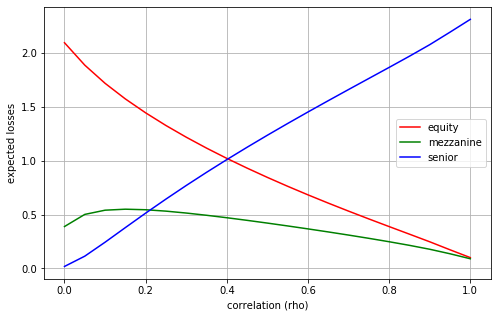
\includegraphics{figures/losses_vs_rho_2}

To demonstrate that the total expected loss is independent from $\rho$ it is enough to print its values for a couple of different values of the correlation parameter. Since the expected loss of the tranches have been saved into lists the sum can be done among values of the lists with similar indices. 

\begin{tcolorbox}[size=fbox, boxrule=1pt, colback=cellbackground, colframe=cellborder]
\begin{Verbatim}[commandchars=\\\{\}]
\PY{n+nb}{print} \PY{p}{(}\PY{n}{res}\PY{p}{[}\PY{l+m+mi}{0}\PY{p}{]}\PY{p}{[}\PY{l+m+mi}{5}\PY{p}{]} \PY{o}{+} \PY{n}{res}\PY{p}{[}\PY{l+m+mi}{1}\PY{p}{]}\PY{p}{[}\PY{l+m+mi}{5}\PY{p}{]} \PY{o}{+} \PY{n}{res}\PY{p}{[}\PY{l+m+mi}{2}\PY{p}{]}\PY{p}{[}\PY{l+m+mi}{5}\PY{p}{]}\PY{p}{)}
\PY{n+nb}{print} \PY{p}{(}\PY{n}{res}\PY{p}{[}\PY{l+m+mi}{0}\PY{p}{]}\PY{p}{[}\PY{l+m+mi}{10}\PY{p}{]} \PY{o}{+} \PY{n}{res}\PY{p}{[}\PY{l+m+mi}{1}\PY{p}{]}\PY{p}{[}\PY{l+m+mi}{10}\PY{p}{]} \PY{o}{+} \PY{n}{res}\PY{p}{[}\PY{l+m+mi}{2}\PY{p}{]}\PY{p}{[}\PY{l+m+mi}{10}\PY{p}{]}\PY{p}{)}
\PY{n+nb}{print} \PY{p}{(}\PY{n}{res}\PY{p}{[}\PY{l+m+mi}{0}\PY{p}{]}\PY{p}{[}\PY{l+m+mi}{15}\PY{p}{]} \PY{o}{+} \PY{n}{res}\PY{p}{[}\PY{l+m+mi}{1}\PY{p}{]}\PY{p}{[}\PY{l+m+mi}{15}\PY{p}{]} \PY{o}{+} \PY{n}{res}\PY{p}{[}\PY{l+m+mi}{2}\PY{p}{]}\PY{p}{[}\PY{l+m+mi}{15}\PY{p}{]}\PY{p}{)}

2.4999999999999725
2.499999999999975
2.4999999999999774
\end{Verbatim}
\end{tcolorbox}
\end{Answer}

\begin{Exercise}[title={(Synthetic CDO)}]
Using the \texttt{CollDebtObligation} class in the \texttt{finmarkets} module determine the fair value of each tranche in a CDO with 1 year maturity and a reference portfolio of 125 names. Each of them have the same default probabilities, 1\% and the correlation is set to 0.2. The tenor of the premium leg is 12 months. The risk free rate is flat at 5\%.
\begin{itemize}
	\item equity: [0.0, 0.03] (spread 0.20);
	\item mezzanine: [0.03, 0.06] (spread 0.01);
	\item senior: [0.06, 1.0] (spread 0.005).
\end{itemize}

How does these results change if the default probability raises to 5\% ?

How does these results change if instead there is an higher correlation (0.6) ?
\end{Exercise}
\begin{Answer}
\begin{tcolorbox}[size=fbox, boxrule=1pt, colback=cellbackground, colframe=cellborder]
\begin{Verbatim}[commandchars=\\\{\}]
\PY{k+kn}{from} \PY{n+nn}{finmarkets} \PY{k}{import} \PY{n}{DiscountCurve}\PY{p}{,} \PY{n}{CreditCurve}\PY{p}{,} \PY{n}{CollDebtObligation}
\PY{k+kn}{from} \PY{n+nn}{datetime} \PY{k}{import} \PY{n}{date}
\PY{k+kn}{from} \PY{n+nn}{dateutil}\PY{n+nn}{.}\PY{n+nn}{relativedelta} \PY{k}{import} \PY{n}{relativedelta}

\PY{n}{pillar\PYZus{}dates} \PY{o}{=} \PY{p}{[}\PY{p}{]}
\PY{n}{df} \PY{o}{=} \PY{p}{[}\PY{p}{]}
\PY{n}{observation\PYZus{}date} \PY{o}{=} \PY{n}{date}\PY{o}{.}\PY{n}{today}\PY{p}{(}\PY{p}{)}
			
\PY{k}{for} \PY{n}{i} \PY{o+ow}{in} \PY{n+nb}{range}\PY{p}{(}\PY{l+m+mi}{2}\PY{p}{)}\PY{p}{:}
	\PY{n}{pillar\PYZus{}dates}\PY{o}{.}\PY{n}{append}\PY{p}{(}\PY{n}{observation\PYZus{}date} \PY{o}{+} \PY{n}{relativedelta}\PY{p}{(}\PY{n}{years}\PY{o}{=}\PY{n}{i}\PY{p}{)}\PY{p}{)}
	\PY{n}{df}\PY{o}{.}\PY{n}{append}\PY{p}{(}\PY{l+m+mi}{1} \PY{o}{/} \PY{p}{(}\PY{l+m+mi}{1} \PY{o}{+} \PY{l+m+mf}{0.05}\PY{p}{)} \PY{o}{*}\PY{o}{*} \PY{n}{i}\PY{p}{)}
\PY{n}{dc} \PY{o}{=} \PY{n}{DiscountCurve}\PY{p}{(}\PY{n}{observation\PYZus{}date}\PY{p}{,} \PY{n}{pillar\PYZus{}dates}\PY{p}{,} \PY{n}{df}\PY{p}{)}
			
\PY{n}{cc} \PY{o}{=} \PY{n}{CreditCurve}\PY{p}{(}\PY{p}{[}\PY{n}{observation\PYZus{}date} \PY{o}{+} \PY{n}{relativedelta}\PY{p}{(}\PY{n}{years}\PY{o}{=}\PY{n}{i}\PY{p}{)} \PY{k}{for} \PY{n}{i} \PY{o+ow}{in} \PY{n+nb}{range}\PY{p}{(}\PY{l+m+mi}{5}\PY{p}{)}\PY{p}{]}\PY{p}{,}
\PY{p}{[}\PY{l+m+mi}{1}\PY{p}{,} \PY{l+m+mf}{0.99}\PY{p}{,} \PY{l+m+mf}{0.97}\PY{p}{,} \PY{l+m+mf}{0.95}\PY{p}{,} \PY{l+m+mf}{0.93}\PY{p}{]}\PY{p}{)}
			
\PY{n}{tranches} \PY{o}{=} \PY{p}{[}\PY{p}{[}\PY{l+m+mf}{0.0}\PY{p}{,} \PY{l+m+mf}{0.03}\PY{p}{]}\PY{p}{,} \PY{p}{[}\PY{l+m+mf}{0.03}\PY{p}{,} \PY{l+m+mf}{0.06}\PY{p}{]}\PY{p}{,} \PY{p}{[}\PY{l+m+mf}{0.06}\PY{p}{,} \PY{l+m+mf}{0.09}\PY{p}{]}\PY{p}{,} \PY{p}{[}\PY{l+m+mf}{0.09}\PY{p}{,} \PY{l+m+mf}{1.0}\PY{p}{]}\PY{p}{]}
\PY{n}{spreads} \PY{o}{=} \PY{p}{[}\PY{l+m+mf}{0.15}\PY{p}{,} \PY{l+m+mf}{0.07}\PY{p}{,} \PY{l+m+mf}{0.03}\PY{p}{,} \PY{l+m+mf}{0.01}\PY{p}{]}
			
\PY{n}{cdo} \PY{o}{=} \PY{n}{CollDebtObligation}\PY{p}{(}\PY{l+m+mf}{100e6}\PY{p}{,} \PY{l+m+mi}{125}\PY{p}{,} \PY{n}{tranches}\PY{p}{,} \PY{l+m+mf}{0.3}\PY{p}{,} \PY{n}{cc}\PY{p}{,}
\PY{n}{observation\PYZus{}date}\PY{p}{,} \PY{n}{spreads}\PY{p}{,} \PY{l+m+mi}{1}\PY{p}{,} \PY{l+m+mi}{12}\PY{p}{)}
\PY{k}{for} \PY{n}{i} \PY{o+ow}{in} \PY{n+nb}{range}\PY{p}{(}\PY{n+nb}{len}\PY{p}{(}\PY{n}{tranches}\PY{p}{)}\PY{p}{)}\PY{p}{:}
    \PY{n+nb}{print} \PY{p}{(}\PY{l+s+s2}{\PYZdq{}}\PY{l+s+s2}{Tranche }\PY{l+s+si}{\PYZob{}\PYZcb{}}\PY{l+s+s2}{ (}\PY{l+s+si}{\PYZob{}\PYZcb{}}\PY{l+s+s2}{): }\PY{l+s+si}{\PYZob{}:.5f\PYZcb{}}\PY{l+s+s2}{\PYZdq{}}\PY{o}{.}\PY{n}{format}\PY{p}{(}\PY{n}{i}\PY{p}{,} \PY{n}{tranches}\PY{p}{[}\PY{n}{i}\PY{p}{]}\PY{p}{,} \PY{n}{cdo}\PY{o}{.}\PY{n}{fair\PYZus{}value}\PY{p}{(}\PY{n}{i}\PY{p}{,} \PY{n}{dc}\PY{p}{)}\PY{p}{)}\PY{p}{)}
	
Tranche 0 ([0.0, 0.03]): 0.17775
Tranche 1 ([0.03, 0.06]): 0.01570
Tranche 2 ([0.06, 1.0]): 0.00012
\end{Verbatim}
\end{tcolorbox}

With an higher default probability instead, the NPV of the default leg increases and so does the fair value.

\begin{tcolorbox}[size=fbox, boxrule=1pt, colback=cellbackground, colframe=cellborder]
\begin{Verbatim}[commandchars=\\\{\}]
Tranche 0 ([0.0, 0.03]): 0.59296
Tranche 1 ([0.03, 0.06]): 0.22714
Tranche 2 ([0.06, 1.0]): 0.00530
\end{Verbatim}
\end{tcolorbox}

With a larger correlation finally the probability of multiple defaults increases leading to larger losses in safer tranches. So the fair value increases in mezzanine and senior tranches, but is lower in the equity where the probability of few defaults is reduced.

\begin{tcolorbox}[size=fbox, boxrule=1pt, colback=cellbackground, colframe=cellborder]
\begin{Verbatim}[commandchars=\\\{\}]
Tranche 0 ([0.0, 0.03]): 0.09899
Tranche 1 ([0.03, 0.06]): 0.03498
Tranche 2 ([0.06, 1.0]): 0.00192
\end{Verbatim}
\end{tcolorbox}
\end{Answer}

%\clearpage
%\chapter{VaR and Credit Risk}\label{exercise-13}

\begin{Exercise}[title={(VaR and Historical Series)}]
Given the historical series of three stock prices in the file
\(\href{https://drive.google.com/file/d/1iLCV5zlfNe9eAu_TQwQyZFhvIKR86-vM/view?usp=sharing}{\textrm{historical.csv}}\)
compute the 1-day 95\% VaR for a portfolio consisting of 40 FOX shares, 35 ABC shares 
and 25 CBS shares. 
Today's price is the last entry of the series.

\textbf{Hint:} when simulating the historical scenarios take care of possible NaN values
in the series. 
\end{Exercise}

\begin{Answer}
\begin{tcolorbox}[size=fbox, boxrule=1pt, colback=cellbackground, colframe=cellborder]
\begin{Verbatim}[commandchars=\\\{\}]
\PY{k+kn}{import} \PY{n+nn}{pandas} \PY{k}{as} \PY{n+nn}{pd}
\PY{k+kn}{from} \PY{n+nn}{scipy}\PY{n+nn}{.}\PY{n+nn}{stats} \PY{k}{import} \PY{n}{norm}
		
\PY{n}{df} \PY{o}{=} \PY{n}{pd}\PY{o}{.}\PY{n}{read\PYZus{}csv}\PY{p}{(}\PY{l+s+s2}{\PYZdq{}}\PY{l+s+s2}{historical.csv}\PY{l+s+s2}{\PYZdq{}}\PY{p}{)}
		
\PY{n}{fox} \PY{o}{=} \PY{n}{df}\PY{p}{[}\PY{n}{df}\PY{p}{[}\PY{l+s+s1}{\PYZsq{}}\PY{l+s+s1}{ticker}\PY{l+s+s1}{\PYZsq{}}\PY{p}{]}\PY{o}{==}\PY{l+s+s1}{\PYZsq{}}\PY{l+s+s1}{FOX}\PY{l+s+s1}{\PYZsq{}}\PY{p}{]}\PY{o}{.}\PY{n}{copy}\PY{p}{(}\PY{p}{)}
\PY{n}{cbs} \PY{o}{=} \PY{n}{df}\PY{p}{[}\PY{n}{df}\PY{p}{[}\PY{l+s+s1}{\PYZsq{}}\PY{l+s+s1}{ticker}\PY{l+s+s1}{\PYZsq{}}\PY{p}{]}\PY{o}{==}\PY{l+s+s1}{\PYZsq{}}\PY{l+s+s1}{CBS}\PY{l+s+s1}{\PYZsq{}}\PY{p}{]}\PY{o}{.}\PY{n}{copy}\PY{p}{(}\PY{p}{)}
\PY{n}{abc} \PY{o}{=} \PY{n}{df}\PY{p}{[}\PY{n}{df}\PY{p}{[}\PY{l+s+s1}{\PYZsq{}}\PY{l+s+s1}{ticker}\PY{l+s+s1}{\PYZsq{}}\PY{p}{]}\PY{o}{==}\PY{l+s+s1}{\PYZsq{}}\PY{l+s+s1}{ABC}\PY{l+s+s1}{\PYZsq{}}\PY{p}{]}\PY{o}{.}\PY{n}{copy}\PY{p}{(}\PY{p}{)}
		
\PY{n}{fox}\PY{p}{[}\PY{l+s+s1}{\PYZsq{}}\PY{l+s+s1}{rets}\PY{l+s+s1}{\PYZsq{}}\PY{p}{]} \PY{o}{=} \PY{n}{fox}\PY{p}{[}\PY{l+s+s1}{\PYZsq{}}\PY{l+s+s1}{adj\PYZus{}close}\PY{l+s+s1}{\PYZsq{}}\PY{p}{]}\PY{o}{/}\PY{n}{fox}\PY{p}{[}\PY{l+s+s1}{\PYZsq{}}\PY{l+s+s1}{adj\PYZus{}close}\PY{l+s+s1}{\PYZsq{}}\PY{p}{]}\PY{o}{.}\PY{n}{shift}\PY{p}{(}\PY{l+m+mi}{1}\PY{p}{)} \PY{o}{\PYZhy{}} \PY{l+m+mi}{1} 
\PY{n}{cbs}\PY{p}{[}\PY{l+s+s1}{\PYZsq{}}\PY{l+s+s1}{rets}\PY{l+s+s1}{\PYZsq{}}\PY{p}{]} \PY{o}{=} \PY{n}{cbs}\PY{p}{[}\PY{l+s+s1}{\PYZsq{}}\PY{l+s+s1}{adj\PYZus{}close}\PY{l+s+s1}{\PYZsq{}}\PY{p}{]}\PY{o}{/}\PY{n}{cbs}\PY{p}{[}\PY{l+s+s1}{\PYZsq{}}\PY{l+s+s1}{adj\PYZus{}close}\PY{l+s+s1}{\PYZsq{}}\PY{p}{]}\PY{o}{.}\PY{n}{shift}\PY{p}{(}\PY{l+m+mi}{1}\PY{p}{)} \PY{o}{\PYZhy{}} \PY{l+m+mi}{1} 
\PY{n}{abc}\PY{p}{[}\PY{l+s+s1}{\PYZsq{}}\PY{l+s+s1}{rets}\PY{l+s+s1}{\PYZsq{}}\PY{p}{]} \PY{o}{=} \PY{n}{abc}\PY{p}{[}\PY{l+s+s1}{\PYZsq{}}\PY{l+s+s1}{adj\PYZus{}close}\PY{l+s+s1}{\PYZsq{}}\PY{p}{]}\PY{o}{/}\PY{n}{abc}\PY{p}{[}\PY{l+s+s1}{\PYZsq{}}\PY{l+s+s1}{adj\PYZus{}close}\PY{l+s+s1}{\PYZsq{}}\PY{p}{]}\PY{o}{.}\PY{n}{shift}\PY{p}{(}\PY{l+m+mi}{1}\PY{p}{)} \PY{o}{\PYZhy{}} \PY{l+m+mi}{1} 
		
\PY{n+nb}{print} \PY{p}{(}\PY{n}{fox}\PY{o}{.}\PY{n}{head}\PY{p}{(}\PY{p}{)}\PY{p}{)}

None        date ticker  adj\_close      rets
0     0  2018-03-27    FOX      36.08       NaN
1     1  2018-03-26    FOX      36.58  0.013858
2     2  2018-03-23    FOX      35.45 -0.030891
3     3  2018-03-22    FOX      36.18  0.020592
4     4  2018-03-21    FOX      36.30  0.003317
\end{Verbatim}
\end{tcolorbox}

\begin{tcolorbox}[size=fbox, boxrule=1pt, colback=cellbackground, colframe=cellborder]
\begin{Verbatim}[commandchars=\\\{\}]
\PY{n}{w} \PY{o}{=} \PY{n}{np}\PY{o}{.}\PY{n}{array}\PY{p}{(}\PY{p}{[}\PY{l+m+mf}{0.4}\PY{p}{,} \PY{l+m+mf}{0.35}\PY{p}{,} \PY{l+m+mf}{0.25}\PY{p}{]}\PY{p}{)}
		
\PY{n}{rets} \PY{o}{=} \PY{p}{[}\PY{p}{]}
\PY{k}{for} \PY{n}{i} \PY{o+ow}{in} \PY{n+nb}{range}\PY{p}{(}\PY{l+m+mi}{1}\PY{p}{,} \PY{n+nb}{len}\PY{p}{(}\PY{n}{abc}\PY{p}{)}\PY{p}{)}\PY{p}{:}
    \PY{n}{ret} \PY{o}{=} \PY{p}{[}\PY{n}{fox}\PY{o}{.}\PY{n}{iloc}\PY{p}{[}\PY{n}{i}\PY{p}{]}\PY{p}{[}\PY{l+s+s1}{\PYZsq{}}\PY{l+s+s1}{rets}\PY{l+s+s1}{\PYZsq{}}\PY{p}{]}\PY{p}{,}
            \PY{n}{abc}\PY{o}{.}\PY{n}{iloc}\PY{p}{[}\PY{n}{i}\PY{p}{]}\PY{p}{[}\PY{l+s+s1}{\PYZsq{}}\PY{l+s+s1}{rets}\PY{l+s+s1}{\PYZsq{}}\PY{p}{]}\PY{p}{,}
            \PY{n}{cbs}\PY{o}{.}\PY{n}{iloc}\PY{p}{[}\PY{n}{i}\PY{p}{]}\PY{p}{[}\PY{l+s+s1}{\PYZsq{}}\PY{l+s+s1}{rets}\PY{l+s+s1}{\PYZsq{}}\PY{p}{]}\PY{p}{]}
    \PY{k}{if} \PY{n}{np}\PY{o}{.}\PY{n}{NaN} \PY{o+ow}{in} \PY{n}{ret}\PY{p}{:}
        \PY{k}{continue}
    \PY{n}{rets}\PY{o}{.}\PY{n}{append}\PY{p}{(}\PY{n}{w}\PY{p}{[}\PY{l+m+mi}{0}\PY{p}{]}\PY{o}{*}\PY{n}{ret}\PY{p}{[}\PY{l+m+mi}{0}\PY{p}{]} \PY{o}{+} \PY{n}{w}\PY{p}{[}\PY{l+m+mi}{1}\PY{p}{]}\PY{o}{*}\PY{n}{ret}\PY{p}{[}\PY{l+m+mi}{1}\PY{p}{]} \PY{o}{+} \PY{n}{w}\PY{p}{[}\PY{l+m+mi}{2}\PY{p}{]} \PY{o}{*} \PY{n}{ret}\PY{p}{[}\PY{l+m+mi}{2}\PY{p}{]}\PY{p}{)}
			
\PY{n}{current\PYZus{}price} \PY{o}{=} \PY{p}{[}\PY{n}{fox}\PY{o}{.}\PY{n}{iloc}\PY{p}{[}\PY{o}{\PYZhy{}}\PY{l+m+mi}{1}\PY{p}{]}\PY{p}{[}\PY{l+s+s1}{\PYZsq{}}\PY{l+s+s1}{adj\PYZus{}close}\PY{l+s+s1}{\PYZsq{}}\PY{p}{]}\PY{p}{,} 
                 \PY{n}{abc}\PY{o}{.}\PY{n}{iloc}\PY{p}{[}\PY{o}{\PYZhy{}}\PY{l+m+mi}{1}\PY{p}{]}\PY{p}{[}\PY{l+s+s1}{\PYZsq{}}\PY{l+s+s1}{adj\PYZus{}close}\PY{l+s+s1}{\PYZsq{}}\PY{p}{]}\PY{p}{,}
                 \PY{n}{cbs}\PY{o}{.}\PY{n}{iloc}\PY{p}{[}\PY{o}{\PYZhy{}}\PY{l+m+mi}{1}\PY{p}{]}\PY{p}{[}\PY{l+s+s1}{\PYZsq{}}\PY{l+s+s1}{adj\PYZus{}close}\PY{l+s+s1}{\PYZsq{}}\PY{p}{]}\PY{p}{]}
\PY{n}{portfolio\PYZus{}price} \PY{o}{=} \PY{n}{w}\PY{o}{.}\PY{n}{dot}\PY{p}{(}\PY{n}{current\PYZus{}price}\PY{p}{)}
\PY{n}{hist\PYZus{}var} \PY{o}{=} \PY{n}{portfolio\PYZus{}price}\PY{o}{*}\PY{n}{np}\PY{o}{.}\PY{n}{percentile}\PY{p}{(}\PY{n}{rets}\PY{p}{,} \PY{l+m+mi}{1}\PY{p}{)}

\PY{n+nb}{print} \PY{p}{(}\PY{l+s+s1}{\PYZsq{}}\PY{l+s+s1}{Historical VAR is }\PY{l+s+si}{\PYZob{}:.3f\PYZcb{}}\PY{l+s+s1}{\PYZsq{}}\PY{o}{.}\PY{n}{format}\PY{p}{(}\PY{n}{hist\PYZus{}var}\PY{p}{)}\PY{p}{)}

Historical VAR is -1.385
\end{Verbatim}
\end{tcolorbox}

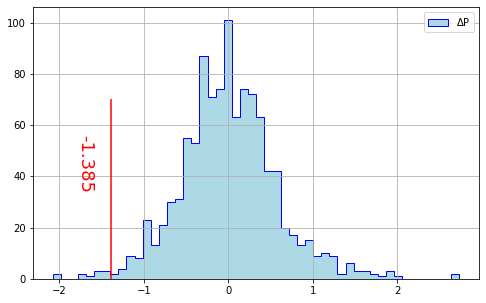
\includegraphics{figures/hist_var_ex}
\end{Answer}

\begin{Exercise}[title={(Credit Valuation Adjustment)}]
You have a 3-years call with strike \euro{110}. The underlying initial price is \euro{100} and the mean rate of return is 0.05 with a volatility of 0.15. The risk-free rate is 0.03 flat.
Compute the CVA of the contract assuming a recovery rate of 40\% and default probabilities for the underlying of 10\%, 20\% and 30\% for first, second and third year respectively.
\end{Exercise}

\begin{Answer}
Below ten simulations of the underlying price in the next three years.

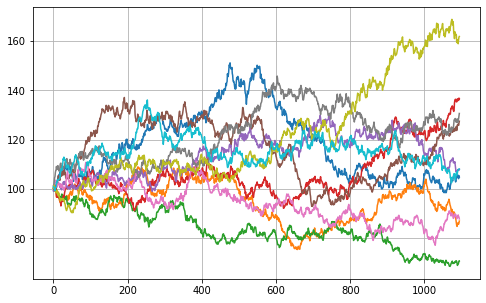
\includegraphics{figures/underlying_simulation}

This is a first implementation of the CVA calculation, not optimized in terms of speed. It takes about 700 seconds to run 1000 simulations.

\begin{tcolorbox}[size=fbox, boxrule=1pt, colback=cellbackground, colframe=cellborder]
\begin{Verbatim}[commandchars=\\\{\}]
\PY{k+kn}{from} \PY{n+nn}{datetime} \PY{k}{import} \PY{n}{date}
\PY{k+kn}{from} \PY{n+nn}{dateutil}\PY{n+nn}{.}\PY{n+nn}{relativedelta} \PY{k}{import} \PY{n}{relativedelta}
\PY{k+kn}{from} \PY{n+nn}{finmarkets} \PY{k}{import} \PY{n}{call\PYZus{}price}\PY{p}{,} \PY{n}{CreditCurve}
\PY{k+kn}{from} \PY{n+nn}{scipy}\PY{n+nn}{.}\PY{n+nn}{stats} \PY{k}{import} \PY{n}{norm}
\PY{k+kn}{import} \PY{n+nn}{numpy} \PY{k}{as} \PY{n+nn}{np}
		
\PY{n}{np}\PY{o}{.}\PY{n}{random}\PY{o}{.}\PY{n}{seed}\PY{p}{(}\PY{l+m+mi}{1}\PY{p}{)}
\PY{n}{dt} \PY{o}{=} \PY{l+m+mi}{1}\PY{o}{/}\PY{l+m+mi}{365}
\PY{n}{K} \PY{o}{=} \PY{l+m+mi}{110}
\PY{n}{sigma} \PY{o}{=} \PY{l+m+mf}{0.15}
\PY{n}{mu} \PY{o}{=} \PY{l+m+mf}{0.05}
\PY{n}{r} \PY{o}{=} \PY{l+m+mf}{0.03}
\PY{n}{T} \PY{o}{=} \PY{l+m+mi}{3}
\PY{n}{R} \PY{o}{=} \PY{l+m+mf}{0.4}
\PY{n}{S} \PY{o}{=} \PY{p}{[}\PY{l+m+mi}{1}\PY{p}{,} \PY{l+m+mf}{0.9}\PY{p}{,} \PY{l+m+mf}{0.8}\PY{p}{,} \PY{l+m+mf}{0.7}\PY{p}{]}
\PY{n}{obs\PYZus{}date} \PY{o}{=} \PY{n}{date}\PY{o}{.}\PY{n}{today}\PY{p}{(}\PY{p}{)}
\PY{n}{pillars} \PY{o}{=} \PY{p}{[}\PY{n}{obs\PYZus{}date} \PY{o}{+} \PY{n}{relativedelta}\PY{p}{(}\PY{n}{years}\PY{o}{=}\PY{n}{i}\PY{p}{)} \PY{k}{for} \PY{n}{i} \PY{o+ow}{in} \PY{n+nb}{range}\PY{p}{(}\PY{n}{T}\PY{o}{+}\PY{l+m+mi}{1}\PY{p}{)}\PY{p}{]}
\PY{n}{cc} \PY{o}{=} \PY{n}{CreditCurve}\PY{p}{(}\PY{n}{pillars}\PY{p}{,} \PY{n}{S}\PY{p}{)}
		
\PY{k+kn}{import} \PY{n+nn}{time}
\PY{n}{t1} \PY{o}{=} \PY{n}{time}\PY{o}{.}\PY{n}{time}\PY{p}{(}\PY{p}{)}
\PY{n}{scenarios} \PY{o}{=} \PY{l+m+mi}{1000}
\PY{n}{cvas} \PY{o}{=} \PY{p}{[}\PY{p}{]}
\end{Verbatim}
\end{tcolorbox}

\begin{tcolorbox}[size=fbox, boxrule=1pt, colback=cellbackground, colframe=cellborder]
\begin{Verbatim}[commandchars=\\\{\}]
\PY{n}{St} \PY{o}{=} \PY{n}{S0}\PY{o}{*}\PY{n}{np}\PY{o}{.}\PY{n}{ones}\PY{p}{(}\PY{n}{shape}\PY{o}{=}\PY{p}{(}\PY{n}{T}\PY{o}{*}\PY{l+m+mi}{365}\PY{p}{,} \PY{n}{scenarios}\PY{p}{)}\PY{p}{)}    
\PY{k}{for} \PY{n}{s} \PY{o+ow}{in} \PY{n+nb}{range}\PY{p}{(}\PY{n}{scenarios}\PY{p}{)}\PY{p}{:}
    \PY{n}{cva} \PY{o}{=} \PY{l+m+mi}{0}
    \PY{n}{St} \PY{o}{=} \PY{l+m+mi}{100}
    \PY{k}{for} \PY{n}{t} \PY{o+ow}{in} \PY{n+nb}{range}\PY{p}{(}\PY{l+m+mi}{0}\PY{p}{,} \PY{l+m+mi}{365}\PY{o}{*}\PY{n}{T}\PY{p}{)}\PY{p}{:} 
        \PY{n}{St} \PY{o}{=} \PY{n}{St} \PY{o}{*} \PY{n}{np}\PY{o}{.}\PY{n}{exp}\PY{p}{(}\PY{p}{(}\PY{n}{mu} \PY{o}{\PYZhy{}} \PY{l+m+mf}{0.5} \PY{o}{*} \PY{n}{sigma}\PY{o}{*}\PY{o}{*}\PY{l+m+mi}{2}\PY{p}{)} \PY{o}{*} \PY{n}{dt} \PY{o}{+} \PY{n}{sigma} 
                \PY{o}{*} \PY{n}{np}\PY{o}{.}\PY{n}{sqrt}\PY{p}{(}\PY{n}{dt}\PY{p}{)} \PY{o}{*} \PY{n}{norm}\PY{o}{.}\PY{n}{rvs}\PY{p}{(}\PY{n}{size}\PY{o}{=}\PY{l+m+mi}{1}\PY{p}{)}\PY{p}{)}
        \PY{n}{cva} \PY{o}{+}\PY{o}{=} \PY{n}{call\PYZus{}price}\PY{p}{(}\PY{n}{dt}\PY{o}{*}\PY{n}{t}\PY{p}{,} \PY{n}{St}\PY{p}{,} \PY{n}{K}\PY{p}{,} \PY{n}{r}\PY{p}{,} \PY{n}{sigma}\PY{p}{,} \PY{n}{T}\PY{p}{)}
                         \PY{o}{*}\PY{p}{(}\PY{n}{cc}\PY{o}{.}\PY{n}{ndp}\PY{p}{(}\PY{n}{obs\PYZus{}date}\PY{o}{+}\PY{n}{relativedelta}\PY{p}{(}\PY{n}{days}\PY{o}{=}\PY{n}{t}\PY{p}{)}\PY{p}{)}\PY{o}{\PYZhy{}}
                         \PY{n}{cc}\PY{o}{.}\PY{n}{ndp}\PY{p}{(}\PY{n}{obs\PYZus{}date}\PY{o}{+}\PY{n}{relativedelta}\PY{p}{(}\PY{n}{days}\PY{o}{=}\PY{n}{t}\PY{o}{+}\PY{l+m+mi}{1}\PY{p}{)}\PY{p}{)}\PY{p}{)}        
    \PY{n}{cvas}\PY{o}{.}\PY{n}{append}\PY{p}{(}\PY{n}{cva}\PY{o}{*}\PY{p}{(}\PY{l+m+mi}{1}\PY{o}{\PYZhy{}}\PY{n}{R}\PY{p}{)}\PY{p}{)}
		
\PY{n+nb}{print} \PY{p}{(}\PY{n}{np}\PY{o}{.}\PY{n}{mean}\PY{p}{(}\PY{n}{cvas}\PY{p}{)}\PY{p}{)}
\PY{n+nb}{print} \PY{p}{(}\PY{n}{time}\PY{o}{.}\PY{n}{time}\PY{p}{(}\PY{p}{)}\PY{o}{\PYZhy{}}\PY{n}{t1}\PY{p}{)}
\end{Verbatim}
\end{tcolorbox}

The next implementation, the one actually used, exploits the \texttt{numpy.array} and it is about 30\% faster.

\begin{tcolorbox}[size=fbox, boxrule=1pt, colback=cellbackground, colframe=cellborder]
\begin{Verbatim}[commandchars=\\\{\}]
\PY{k+kn}{from} \PY{n+nn}{datetime} \PY{k}{import} \PY{n}{date}
\PY{k+kn}{from} \PY{n+nn}{dateutil}\PY{n+nn}{.}\PY{n+nn}{relativedelta} \PY{k}{import} \PY{n}{relativedelta}
\PY{k+kn}{from} \PY{n+nn}{finmarkets} \PY{k}{import} \PY{n}{call\PYZus{}price}\PY{p}{,} \PY{n}{CreditCurve}
\PY{k+kn}{from} \PY{n+nn}{scipy}\PY{n+nn}{.}\PY{n+nn}{stats} \PY{k}{import} \PY{n}{norm}
\PY{k+kn}{import} \PY{n+nn}{numpy} \PY{k}{as} \PY{n+nn}{np}
		
\PY{n}{np}\PY{o}{.}\PY{n}{random}\PY{o}{.}\PY{n}{seed}\PY{p}{(}\PY{l+m+mi}{1}\PY{p}{)}
\PY{n}{dt} \PY{o}{=} \PY{l+m+mi}{1}\PY{o}{/}\PY{l+m+mi}{365}
\PY{n}{K} \PY{o}{=} \PY{l+m+mi}{110}
\PY{n}{sigma} \PY{o}{=} \PY{l+m+mf}{0.15}
\PY{n}{mu} \PY{o}{=} \PY{l+m+mf}{0.05}
\PY{n}{r} \PY{o}{=} \PY{l+m+mf}{0.03}
\PY{n}{T} \PY{o}{=} \PY{l+m+mi}{3}
\PY{n}{R} \PY{o}{=} \PY{l+m+mf}{0.4}
\PY{n}{S} \PY{o}{=} \PY{p}{[}\PY{l+m+mi}{1}\PY{p}{,} \PY{l+m+mf}{0.9}\PY{p}{,} \PY{l+m+mf}{0.8}\PY{p}{,} \PY{l+m+mf}{0.7}\PY{p}{]}
\PY{n}{obs\PYZus{}date} \PY{o}{=} \PY{n}{date}\PY{o}{.}\PY{n}{today}\PY{p}{(}\PY{p}{)}
\PY{n}{pillars} \PY{o}{=} \PY{p}{[}\PY{n}{obs\PYZus{}date} \PY{o}{+} \PY{n}{relativedelta}\PY{p}{(}\PY{n}{years}\PY{o}{=}\PY{n}{i}\PY{p}{)} \PY{k}{for} \PY{n}{i} \PY{o+ow}{in} \PY{n+nb}{range}\PY{p}{(}\PY{n}{T}\PY{o}{+}\PY{l+m+mi}{1}\PY{p}{)}\PY{p}{]}
\PY{n}{cc} \PY{o}{=} \PY{n}{CreditCurve}\PY{p}{(}\PY{n}{pillars}\PY{p}{,} \PY{n}{S}\PY{p}{)}
		
\PY{k+kn}{import} \PY{n+nn}{time}
\PY{n}{t1} \PY{o}{=} \PY{n}{time}\PY{o}{.}\PY{n}{time}\PY{p}{(}\PY{p}{)}
\PY{n}{scenarios} \PY{o}{=} \PY{l+m+mi}{1000}
\PY{n}{cvas} \PY{o}{=} \PY{p}{[}\PY{p}{]}
		
\PY{n}{St} \PY{o}{=} \PY{n}{S0}\PY{o}{*}\PY{n}{np}\PY{o}{.}\PY{n}{ones}\PY{p}{(}\PY{n}{shape}\PY{o}{=}\PY{p}{(}\PY{n}{T}\PY{o}{*}\PY{l+m+mi}{365}\PY{p}{,} \PY{n}{scenarios}\PY{p}{)}\PY{p}{)}    
\PY{k}{for} \PY{n}{i} \PY{o+ow}{in} \PY{n+nb}{range}\PY{p}{(}\PY{n}{T}\PY{o}{*}\PY{l+m+mi}{365}\PY{p}{)}\PY{p}{:}
    \PY{n}{norms} \PY{o}{=} \PY{n}{norm}\PY{o}{.}\PY{n}{rvs}\PY{p}{(}\PY{n}{size}\PY{o}{=}\PY{n}{scenarios}\PY{p}{)}
    \PY{n}{St}\PY{p}{[}\PY{n}{i}\PY{p}{,} \PY{p}{:}\PY{p}{]} \PY{o}{=} \PY{n}{St}\PY{p}{[}\PY{n}{i}\PY{o}{\PYZhy{}}\PY{l+m+mi}{1}\PY{p}{,} \PY{p}{:}\PY{p}{]} \PY{o}{*} \PY{n}{np}\PY{o}{.}\PY{n}{exp}\PY{p}{(}\PY{p}{(}\PY{n}{mu} \PY{o}{\PYZhy{}} \PY{l+m+mf}{0.5} \PY{o}{*} \PY{n}{sigma}\PY{o}{*}\PY{o}{*}\PY{l+m+mi}{2}\PY{p}{)} \PY{o}{*} \PY{n}{dt} \PY{o}{+} \PY{n}{sigma}
                          \PY{o}{*} \PY{n}{np}\PY{o}{.}\PY{n}{sqrt}\PY{p}{(}\PY{n}{dt}\PY{p}{)} \PY{o}{*} \PY{n}{norms}\PY{p}{[}\PY{p}{:}\PY{p}{]}\PY{p}{)}
\end{Verbatim}
\end{tcolorbox}

\begin{tcolorbox}[size=fbox, boxrule=1pt, colback=cellbackground, colframe=cellborder]
\begin{Verbatim}[commandchars=\\\{\}]
	
\PY{k}{for} \PY{n}{s} \PY{o+ow}{in} \PY{n+nb}{range}\PY{p}{(}\PY{n}{scenarios}\PY{p}{)}\PY{p}{:}
    \PY{n}{cva} \PY{o}{=} \PY{l+m+mi}{0}
    \PY{k}{for} \PY{n}{t} \PY{o+ow}{in} \PY{n+nb}{range}\PY{p}{(}\PY{l+m+mi}{365}\PY{o}{*}\PY{n}{T}\PY{p}{)}\PY{p}{:} 
        \PY{n}{cva} \PY{o}{+}\PY{o}{=} \PY{n}{call\PYZus{}price}\PY{p}{(}\PY{n}{dt}\PY{o}{*}\PY{n}{t}\PY{p}{,} \PY{n}{St}\PY{p}{[}\PY{n}{i}\PY{p}{,} \PY{n}{s}\PY{p}{]}\PY{p}{,} \PY{n}{K}\PY{p}{,} \PY{n}{r}\PY{p}{,} \PY{n}{sigma}\PY{p}{,} \PY{n}{T}\PY{p}{)}\PY{o}{*} \PYZbs{}
                           \PY{p}{(}\PY{n}{cc}\PY{o}{.}\PY{n}{ndp}\PY{p}{(}\PY{n}{obs\PYZus{}date}\PY{o}{+}\PY{n}{relativedelta}\PY{p}{(}\PY{n}{days}\PY{o}{=}\PY{n}{t}\PY{p}{)}\PY{p}{)}\PY{o}{\PYZhy{}}
                           \PY{n}{cc}\PY{o}{.}\PY{n}{ndp}\PY{p}{(}\PY{n}{obs\PYZus{}date}\PY{o}{+}\PY{n}{relativedelta}\PY{p}{(}\PY{n}{days}\PY{o}{=}\PY{n}{t}\PY{o}{+}\PY{l+m+mi}{1}\PY{p}{)}\PY{p}{)}\PY{p}{)}        
    \PY{n}{cvas}\PY{o}{.}\PY{n}{append}\PY{p}{(}\PY{n}{cva}\PY{o}{*}\PY{p}{(}\PY{l+m+mi}{1}\PY{o}{\PYZhy{}}\PY{n}{R}\PY{p}{)}\PY{p}{)}
				
\PY{n+nb}{print} \PY{p}{(}\PY{n}{np}\PY{o}{.}\PY{n}{mean}\PY{p}{(}\PY{n}{cvas}\PY{p}{)}\PY{p}{)}
\PY{n+nb}{print} \PY{p}{(}\PY{n}{time}\PY{o}{.}\PY{n}{time}\PY{p}{(}\PY{p}{)}\PY{o}{\PYZhy{}}\PY{n}{t1}\PY{p}{)}

3.7521017896018973
459.46695613861084
\end{Verbatim}
\end{tcolorbox}
\end{Answer}

\begin{Exercise}[title={(Credit VaR)}]
Consider a 1-years call with strike \euro{110}. The underlying initial price is \euro{100} and the mean rate of return is 0.05 with a volatility of 0.15. The risk-free rate is 0.03 flat.
Compute the 99.9\% Credit VaR assuming a recovery rate of 40\% and default probabilities for the underlying of 30\% within next year.
\end{Exercise}

\begin{Answer}
\begin{tcolorbox}[size=fbox, boxrule=1pt, colback=cellbackground, colframe=cellborder]
\begin{Verbatim}[commandchars=\\\{\}]
\PY{c+c1}{\PYZsh{} 460s for 1000 simulations}
\PY{k+kn}{from} \PY{n+nn}{datetime} \PY{k}{import} \PY{n}{date}
\PY{k+kn}{from} \PY{n+nn}{dateutil}\PY{n+nn}{.}\PY{n+nn}{relativedelta} \PY{k}{import} \PY{n}{relativedelta}
\PY{k+kn}{from} \PY{n+nn}{finmarkets} \PY{k}{import} \PY{n}{call\PYZus{}price}\PY{p}{,} \PY{n}{CreditCurve}
\PY{k+kn}{from} \PY{n+nn}{scipy}\PY{n+nn}{.}\PY{n+nn}{stats} \PY{k}{import} \PY{n}{norm}
\PY{k+kn}{import} \PY{n+nn}{numpy} \PY{k}{as} \PY{n+nn}{np}
		
\PY{n}{np}\PY{o}{.}\PY{n}{random}\PY{o}{.}\PY{n}{seed}\PY{p}{(}\PY{l+m+mi}{1}\PY{p}{)}
\PY{n}{dt} \PY{o}{=} \PY{l+m+mi}{1}\PY{o}{/}\PY{l+m+mi}{365}
\PY{n}{K} \PY{o}{=} \PY{l+m+mi}{110}
\PY{n}{sigma} \PY{o}{=} \PY{l+m+mf}{0.15}
\PY{n}{mu} \PY{o}{=} \PY{l+m+mf}{0.05}
\PY{n}{r} \PY{o}{=} \PY{l+m+mf}{0.03}
\PY{n}{T} \PY{o}{=} \PY{l+m+mi}{1}
\PY{n}{R} \PY{o}{=} \PY{l+m+mf}{0.4}
\PY{n}{S} \PY{o}{=} \PY{p}{[}\PY{l+m+mi}{1}\PY{p}{,} \PY{l+m+mf}{0.7}\PY{p}{]}
\PY{n}{obs\PYZus{}date} \PY{o}{=} \PY{n}{date}\PY{o}{.}\PY{n}{today}\PY{p}{(}\PY{p}{)}
\PY{n}{pillars} \PY{o}{=} \PY{p}{[}\PY{n}{obs\PYZus{}date} \PY{o}{+} \PY{n}{relativedelta}\PY{p}{(}\PY{n}{years}\PY{o}{=}\PY{n}{i}\PY{p}{)} \PY{k}{for} \PY{n}{i} \PY{o+ow}{in} \PY{n+nb}{range}\PY{p}{(}\PY{n}{T}\PY{o}{+}\PY{l+m+mi}{1}\PY{p}{)}\PY{p}{]}
\PY{n}{cc} \PY{o}{=} \PY{n}{CreditCurve}\PY{p}{(}\PY{n}{pillars}\PY{p}{,} \PY{n}{S}\PY{p}{)}
		
\PY{n}{scenarios} \PY{o}{=} \PY{l+m+mi}{1000}
\PY{n}{losses} \PY{o}{=} \PY{p}{[}\PY{p}{]}
\end{Verbatim}
\end{tcolorbox}		

\begin{tcolorbox}[size=fbox, boxrule=1pt, colback=cellbackground, colframe=cellborder]
\begin{Verbatim}[commandchars=\\\{\}]

\PY{n}{St} \PY{o}{=} \PY{n}{S0}\PY{o}{*}\PY{n}{np}\PY{o}{.}\PY{n}{ones}\PY{p}{(}\PY{n}{shape}\PY{o}{=}\PY{p}{(}\PY{n}{T}\PY{o}{*}\PY{l+m+mi}{365}\PY{p}{,} \PY{n}{scenarios}\PY{p}{)}\PY{p}{)}    
\PY{k}{for} \PY{n}{i} \PY{o+ow}{in} \PY{n+nb}{range}\PY{p}{(}\PY{n}{T}\PY{o}{*}\PY{l+m+mi}{365}\PY{p}{)}\PY{p}{:}
    \PY{n}{norms} \PY{o}{=} \PY{n}{norm}\PY{o}{.}\PY{n}{rvs}\PY{p}{(}\PY{n}{size}\PY{o}{=}\PY{n}{scenarios}\PY{p}{)}
    \PY{n}{St}\PY{p}{[}\PY{n}{i}\PY{p}{,} \PY{p}{:}\PY{p}{]} \PY{o}{=} \PY{n}{St}\PY{p}{[}\PY{n}{i}\PY{o}{\PYZhy{}}\PY{l+m+mi}{1}\PY{p}{,} \PY{p}{:}\PY{p}{]} \PY{o}{*} \PY{n}{np}\PY{o}{.}\PY{n}{exp}\PY{p}{(}\PY{p}{(}\PY{n}{mu} \PY{o}{\PYZhy{}} \PY{l+m+mf}{0.5} \PY{o}{*} \PY{n}{sigma}\PY{o}{*}\PY{o}{*}\PY{l+m+mi}{2}\PY{p}{)} \PY{o}{*} \PY{n}{dt} \PY{o}{+} \PY{n}{sigma}
                         \PY{o}{*} \PY{n}{np}\PY{o}{.}\PY{n}{sqrt}\PY{p}{(}\PY{n}{dt}\PY{p}{)} \PY{o}{*} 	\PY{n}{norms}\PY{p}{[}\PY{p}{:}\PY{p}{]}\PY{p}{)}
		
\PY{k}{for} \PY{n}{s} \PY{o+ow}{in} \PY{n+nb}{range}\PY{p}{(}\PY{n}{scenarios}\PY{p}{)}\PY{p}{:}
    \PY{n}{loss} \PY{o}{=} \PY{l+m+mi}{0}
    \PY{k}{for} \PY{n}{t} \PY{o+ow}{in} \PY{n+nb}{range}\PY{p}{(}\PY{l+m+mi}{365}\PY{o}{*}\PY{n}{T}\PY{p}{)}\PY{p}{:} 
        \PY{n}{loss} \PY{o}{+}\PY{o}{=} \PY{n}{call\PYZus{}price}\PY{p}{(}\PY{n}{dt}\PY{o}{*}\PY{n}{t}\PY{p}{,} \PY{n}{St}\PY{p}{[}\PY{n}{i}\PY{p}{,} \PY{n}{s}\PY{p}{]}\PY{p}{,} \PY{n}{K}\PY{p}{,} \PY{n}{r}\PY{p}{,} \PY{n}{sigma}\PY{p}{,} \PY{n}{T}\PY{p}{)}\PY{o}{*} \PYZbs{}
                            \PY{p}{(}\PY{n}{cc}\PY{o}{.}\PY{n}{ndp}\PY{p}{(}\PY{n}{obs\PYZus{}date}\PY{o}{+}\PY{n}{relativedelta}\PY{p}{(}\PY{n}{days}\PY{o}{=}\PY{n}{t}\PY{p}{)}\PY{p}{)}\PY{o}{\PYZhy{}}
                            \PY{n}{cc}\PY{o}{.}\PY{n}{ndp}\PY{p}{(}\PY{n}{obs\PYZus{}date}\PY{o}{+}\PY{n}{relativedelta}\PY{p}{(}\PY{n}{days}\PY{o}{=}\PY{n}{t}\PY{o}{+}\PY{l+m+mi}{1}\PY{p}{)}\PY{p}{)}\PY{p}{)}        
    \PY{n}{losses}\PY{o}{.}\PY{n}{append}\PY{p}{(}\PY{n}{cva}\PY{o}{*}\PY{p}{(}\PY{l+m+mi}{1}\PY{o}{\PYZhy{}}\PY{n}{R}\PY{p}{)}\PY{p}{)}
		
\PY{n+nb}{print} \PY{p}{(}\PY{n}{np}\PY{o}{.}\PY{n}{percentile}\PY{p}{(}\PY{n}{cvas}\PY{p}{,} \PY{p}{[}\PY{l+m+mf}{99.9}\PY{p}{]}\PY{p}{)}\PY{p}{)}

[9.96586061]
\end{Verbatim}
\end{tcolorbox}

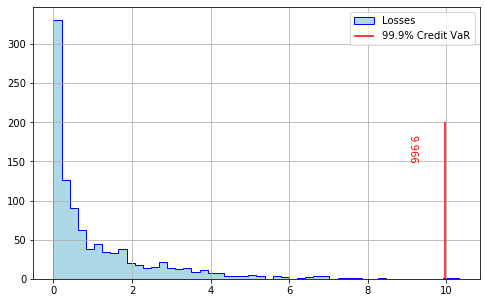
\includegraphics{figures/cr_var_ex}
\end{Answer}






%\clearpage
%\chapter{VaR and Credit Risk}\label{exercise-13}

\begin{Exercise}[title={(VaR and Historical Series)}]
Given the historical series of three stock prices in the file
\(\href{https://drive.google.com/file/d/1iLCV5zlfNe9eAu_TQwQyZFhvIKR86-vM/view?usp=sharing}{\textrm{historical.csv}}\)
compute the 1-day 95\% VaR for a portfolio consisting of 40 FOX shares, 35 ABC shares 
and 25 CBS shares. 
Today's price is the last entry of the series.

\textbf{Hint:} when simulating the historical scenarios take care of possible NaN values
in the series. 
\end{Exercise}

\begin{Answer}
\begin{tcolorbox}[size=fbox, boxrule=1pt, colback=cellbackground, colframe=cellborder]
\begin{Verbatim}[commandchars=\\\{\}]
\PY{k+kn}{import} \PY{n+nn}{pandas} \PY{k}{as} \PY{n+nn}{pd}
\PY{k+kn}{from} \PY{n+nn}{scipy}\PY{n+nn}{.}\PY{n+nn}{stats} \PY{k}{import} \PY{n}{norm}
		
\PY{n}{df} \PY{o}{=} \PY{n}{pd}\PY{o}{.}\PY{n}{read\PYZus{}csv}\PY{p}{(}\PY{l+s+s2}{\PYZdq{}}\PY{l+s+s2}{historical.csv}\PY{l+s+s2}{\PYZdq{}}\PY{p}{)}
		
\PY{n}{fox} \PY{o}{=} \PY{n}{df}\PY{p}{[}\PY{n}{df}\PY{p}{[}\PY{l+s+s1}{\PYZsq{}}\PY{l+s+s1}{ticker}\PY{l+s+s1}{\PYZsq{}}\PY{p}{]}\PY{o}{==}\PY{l+s+s1}{\PYZsq{}}\PY{l+s+s1}{FOX}\PY{l+s+s1}{\PYZsq{}}\PY{p}{]}\PY{o}{.}\PY{n}{copy}\PY{p}{(}\PY{p}{)}
\PY{n}{cbs} \PY{o}{=} \PY{n}{df}\PY{p}{[}\PY{n}{df}\PY{p}{[}\PY{l+s+s1}{\PYZsq{}}\PY{l+s+s1}{ticker}\PY{l+s+s1}{\PYZsq{}}\PY{p}{]}\PY{o}{==}\PY{l+s+s1}{\PYZsq{}}\PY{l+s+s1}{CBS}\PY{l+s+s1}{\PYZsq{}}\PY{p}{]}\PY{o}{.}\PY{n}{copy}\PY{p}{(}\PY{p}{)}
\PY{n}{abc} \PY{o}{=} \PY{n}{df}\PY{p}{[}\PY{n}{df}\PY{p}{[}\PY{l+s+s1}{\PYZsq{}}\PY{l+s+s1}{ticker}\PY{l+s+s1}{\PYZsq{}}\PY{p}{]}\PY{o}{==}\PY{l+s+s1}{\PYZsq{}}\PY{l+s+s1}{ABC}\PY{l+s+s1}{\PYZsq{}}\PY{p}{]}\PY{o}{.}\PY{n}{copy}\PY{p}{(}\PY{p}{)}
		
\PY{n}{fox}\PY{p}{[}\PY{l+s+s1}{\PYZsq{}}\PY{l+s+s1}{rets}\PY{l+s+s1}{\PYZsq{}}\PY{p}{]} \PY{o}{=} \PY{n}{fox}\PY{p}{[}\PY{l+s+s1}{\PYZsq{}}\PY{l+s+s1}{adj\PYZus{}close}\PY{l+s+s1}{\PYZsq{}}\PY{p}{]}\PY{o}{/}\PY{n}{fox}\PY{p}{[}\PY{l+s+s1}{\PYZsq{}}\PY{l+s+s1}{adj\PYZus{}close}\PY{l+s+s1}{\PYZsq{}}\PY{p}{]}\PY{o}{.}\PY{n}{shift}\PY{p}{(}\PY{l+m+mi}{1}\PY{p}{)} \PY{o}{\PYZhy{}} \PY{l+m+mi}{1} 
\PY{n}{cbs}\PY{p}{[}\PY{l+s+s1}{\PYZsq{}}\PY{l+s+s1}{rets}\PY{l+s+s1}{\PYZsq{}}\PY{p}{]} \PY{o}{=} \PY{n}{cbs}\PY{p}{[}\PY{l+s+s1}{\PYZsq{}}\PY{l+s+s1}{adj\PYZus{}close}\PY{l+s+s1}{\PYZsq{}}\PY{p}{]}\PY{o}{/}\PY{n}{cbs}\PY{p}{[}\PY{l+s+s1}{\PYZsq{}}\PY{l+s+s1}{adj\PYZus{}close}\PY{l+s+s1}{\PYZsq{}}\PY{p}{]}\PY{o}{.}\PY{n}{shift}\PY{p}{(}\PY{l+m+mi}{1}\PY{p}{)} \PY{o}{\PYZhy{}} \PY{l+m+mi}{1} 
\PY{n}{abc}\PY{p}{[}\PY{l+s+s1}{\PYZsq{}}\PY{l+s+s1}{rets}\PY{l+s+s1}{\PYZsq{}}\PY{p}{]} \PY{o}{=} \PY{n}{abc}\PY{p}{[}\PY{l+s+s1}{\PYZsq{}}\PY{l+s+s1}{adj\PYZus{}close}\PY{l+s+s1}{\PYZsq{}}\PY{p}{]}\PY{o}{/}\PY{n}{abc}\PY{p}{[}\PY{l+s+s1}{\PYZsq{}}\PY{l+s+s1}{adj\PYZus{}close}\PY{l+s+s1}{\PYZsq{}}\PY{p}{]}\PY{o}{.}\PY{n}{shift}\PY{p}{(}\PY{l+m+mi}{1}\PY{p}{)} \PY{o}{\PYZhy{}} \PY{l+m+mi}{1} 
		
\PY{n+nb}{print} \PY{p}{(}\PY{n}{fox}\PY{o}{.}\PY{n}{head}\PY{p}{(}\PY{p}{)}\PY{p}{)}

None        date ticker  adj\_close      rets
0     0  2018-03-27    FOX      36.08       NaN
1     1  2018-03-26    FOX      36.58  0.013858
2     2  2018-03-23    FOX      35.45 -0.030891
3     3  2018-03-22    FOX      36.18  0.020592
4     4  2018-03-21    FOX      36.30  0.003317
\end{Verbatim}
\end{tcolorbox}

\begin{tcolorbox}[size=fbox, boxrule=1pt, colback=cellbackground, colframe=cellborder]
\begin{Verbatim}[commandchars=\\\{\}]
\PY{n}{w} \PY{o}{=} \PY{n}{np}\PY{o}{.}\PY{n}{array}\PY{p}{(}\PY{p}{[}\PY{l+m+mf}{0.4}\PY{p}{,} \PY{l+m+mf}{0.35}\PY{p}{,} \PY{l+m+mf}{0.25}\PY{p}{]}\PY{p}{)}
		
\PY{n}{rets} \PY{o}{=} \PY{p}{[}\PY{p}{]}
\PY{k}{for} \PY{n}{i} \PY{o+ow}{in} \PY{n+nb}{range}\PY{p}{(}\PY{l+m+mi}{1}\PY{p}{,} \PY{n+nb}{len}\PY{p}{(}\PY{n}{abc}\PY{p}{)}\PY{p}{)}\PY{p}{:}
    \PY{n}{ret} \PY{o}{=} \PY{p}{[}\PY{n}{fox}\PY{o}{.}\PY{n}{iloc}\PY{p}{[}\PY{n}{i}\PY{p}{]}\PY{p}{[}\PY{l+s+s1}{\PYZsq{}}\PY{l+s+s1}{rets}\PY{l+s+s1}{\PYZsq{}}\PY{p}{]}\PY{p}{,}
            \PY{n}{abc}\PY{o}{.}\PY{n}{iloc}\PY{p}{[}\PY{n}{i}\PY{p}{]}\PY{p}{[}\PY{l+s+s1}{\PYZsq{}}\PY{l+s+s1}{rets}\PY{l+s+s1}{\PYZsq{}}\PY{p}{]}\PY{p}{,}
            \PY{n}{cbs}\PY{o}{.}\PY{n}{iloc}\PY{p}{[}\PY{n}{i}\PY{p}{]}\PY{p}{[}\PY{l+s+s1}{\PYZsq{}}\PY{l+s+s1}{rets}\PY{l+s+s1}{\PYZsq{}}\PY{p}{]}\PY{p}{]}
    \PY{k}{if} \PY{n}{np}\PY{o}{.}\PY{n}{NaN} \PY{o+ow}{in} \PY{n}{ret}\PY{p}{:}
        \PY{k}{continue}
    \PY{n}{rets}\PY{o}{.}\PY{n}{append}\PY{p}{(}\PY{n}{w}\PY{p}{[}\PY{l+m+mi}{0}\PY{p}{]}\PY{o}{*}\PY{n}{ret}\PY{p}{[}\PY{l+m+mi}{0}\PY{p}{]} \PY{o}{+} \PY{n}{w}\PY{p}{[}\PY{l+m+mi}{1}\PY{p}{]}\PY{o}{*}\PY{n}{ret}\PY{p}{[}\PY{l+m+mi}{1}\PY{p}{]} \PY{o}{+} \PY{n}{w}\PY{p}{[}\PY{l+m+mi}{2}\PY{p}{]} \PY{o}{*} \PY{n}{ret}\PY{p}{[}\PY{l+m+mi}{2}\PY{p}{]}\PY{p}{)}
			
\PY{n}{current\PYZus{}price} \PY{o}{=} \PY{p}{[}\PY{n}{fox}\PY{o}{.}\PY{n}{iloc}\PY{p}{[}\PY{o}{\PYZhy{}}\PY{l+m+mi}{1}\PY{p}{]}\PY{p}{[}\PY{l+s+s1}{\PYZsq{}}\PY{l+s+s1}{adj\PYZus{}close}\PY{l+s+s1}{\PYZsq{}}\PY{p}{]}\PY{p}{,} 
                 \PY{n}{abc}\PY{o}{.}\PY{n}{iloc}\PY{p}{[}\PY{o}{\PYZhy{}}\PY{l+m+mi}{1}\PY{p}{]}\PY{p}{[}\PY{l+s+s1}{\PYZsq{}}\PY{l+s+s1}{adj\PYZus{}close}\PY{l+s+s1}{\PYZsq{}}\PY{p}{]}\PY{p}{,}
                 \PY{n}{cbs}\PY{o}{.}\PY{n}{iloc}\PY{p}{[}\PY{o}{\PYZhy{}}\PY{l+m+mi}{1}\PY{p}{]}\PY{p}{[}\PY{l+s+s1}{\PYZsq{}}\PY{l+s+s1}{adj\PYZus{}close}\PY{l+s+s1}{\PYZsq{}}\PY{p}{]}\PY{p}{]}
\PY{n}{portfolio\PYZus{}price} \PY{o}{=} \PY{n}{w}\PY{o}{.}\PY{n}{dot}\PY{p}{(}\PY{n}{current\PYZus{}price}\PY{p}{)}
\PY{n}{hist\PYZus{}var} \PY{o}{=} \PY{n}{portfolio\PYZus{}price}\PY{o}{*}\PY{n}{np}\PY{o}{.}\PY{n}{percentile}\PY{p}{(}\PY{n}{rets}\PY{p}{,} \PY{l+m+mi}{1}\PY{p}{)}

\PY{n+nb}{print} \PY{p}{(}\PY{l+s+s1}{\PYZsq{}}\PY{l+s+s1}{Historical VAR is }\PY{l+s+si}{\PYZob{}:.3f\PYZcb{}}\PY{l+s+s1}{\PYZsq{}}\PY{o}{.}\PY{n}{format}\PY{p}{(}\PY{n}{hist\PYZus{}var}\PY{p}{)}\PY{p}{)}

Historical VAR is -1.385
\end{Verbatim}
\end{tcolorbox}

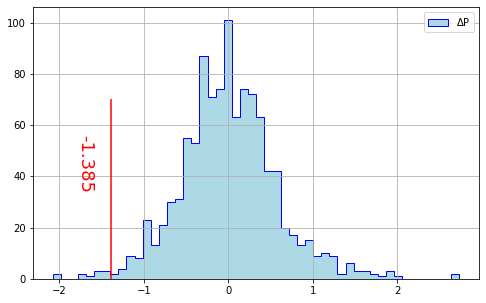
\includegraphics{figures/hist_var_ex}
\end{Answer}

\begin{Exercise}[title={(Credit Valuation Adjustment)}]
You have a 3-years call with strike \euro{110}. The underlying initial price is \euro{100} and the mean rate of return is 0.05 with a volatility of 0.15. The risk-free rate is 0.03 flat.
Compute the CVA of the contract assuming a recovery rate of 40\% and default probabilities for the underlying of 10\%, 20\% and 30\% for first, second and third year respectively.
\end{Exercise}

\begin{Answer}
Below ten simulations of the underlying price in the next three years.

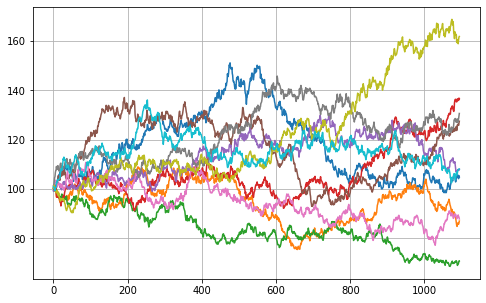
\includegraphics{figures/underlying_simulation}

This is a first implementation of the CVA calculation, not optimized in terms of speed. It takes about 700 seconds to run 1000 simulations.

\begin{tcolorbox}[size=fbox, boxrule=1pt, colback=cellbackground, colframe=cellborder]
\begin{Verbatim}[commandchars=\\\{\}]
\PY{k+kn}{from} \PY{n+nn}{datetime} \PY{k}{import} \PY{n}{date}
\PY{k+kn}{from} \PY{n+nn}{dateutil}\PY{n+nn}{.}\PY{n+nn}{relativedelta} \PY{k}{import} \PY{n}{relativedelta}
\PY{k+kn}{from} \PY{n+nn}{finmarkets} \PY{k}{import} \PY{n}{call\PYZus{}price}\PY{p}{,} \PY{n}{CreditCurve}
\PY{k+kn}{from} \PY{n+nn}{scipy}\PY{n+nn}{.}\PY{n+nn}{stats} \PY{k}{import} \PY{n}{norm}
\PY{k+kn}{import} \PY{n+nn}{numpy} \PY{k}{as} \PY{n+nn}{np}
		
\PY{n}{np}\PY{o}{.}\PY{n}{random}\PY{o}{.}\PY{n}{seed}\PY{p}{(}\PY{l+m+mi}{1}\PY{p}{)}
\PY{n}{dt} \PY{o}{=} \PY{l+m+mi}{1}\PY{o}{/}\PY{l+m+mi}{365}
\PY{n}{K} \PY{o}{=} \PY{l+m+mi}{110}
\PY{n}{sigma} \PY{o}{=} \PY{l+m+mf}{0.15}
\PY{n}{mu} \PY{o}{=} \PY{l+m+mf}{0.05}
\PY{n}{r} \PY{o}{=} \PY{l+m+mf}{0.03}
\PY{n}{T} \PY{o}{=} \PY{l+m+mi}{3}
\PY{n}{R} \PY{o}{=} \PY{l+m+mf}{0.4}
\PY{n}{S} \PY{o}{=} \PY{p}{[}\PY{l+m+mi}{1}\PY{p}{,} \PY{l+m+mf}{0.9}\PY{p}{,} \PY{l+m+mf}{0.8}\PY{p}{,} \PY{l+m+mf}{0.7}\PY{p}{]}
\PY{n}{obs\PYZus{}date} \PY{o}{=} \PY{n}{date}\PY{o}{.}\PY{n}{today}\PY{p}{(}\PY{p}{)}
\PY{n}{pillars} \PY{o}{=} \PY{p}{[}\PY{n}{obs\PYZus{}date} \PY{o}{+} \PY{n}{relativedelta}\PY{p}{(}\PY{n}{years}\PY{o}{=}\PY{n}{i}\PY{p}{)} \PY{k}{for} \PY{n}{i} \PY{o+ow}{in} \PY{n+nb}{range}\PY{p}{(}\PY{n}{T}\PY{o}{+}\PY{l+m+mi}{1}\PY{p}{)}\PY{p}{]}
\PY{n}{cc} \PY{o}{=} \PY{n}{CreditCurve}\PY{p}{(}\PY{n}{pillars}\PY{p}{,} \PY{n}{S}\PY{p}{)}
		
\PY{k+kn}{import} \PY{n+nn}{time}
\PY{n}{t1} \PY{o}{=} \PY{n}{time}\PY{o}{.}\PY{n}{time}\PY{p}{(}\PY{p}{)}
\PY{n}{scenarios} \PY{o}{=} \PY{l+m+mi}{1000}
\PY{n}{cvas} \PY{o}{=} \PY{p}{[}\PY{p}{]}
\end{Verbatim}
\end{tcolorbox}

\begin{tcolorbox}[size=fbox, boxrule=1pt, colback=cellbackground, colframe=cellborder]
\begin{Verbatim}[commandchars=\\\{\}]
\PY{n}{St} \PY{o}{=} \PY{n}{S0}\PY{o}{*}\PY{n}{np}\PY{o}{.}\PY{n}{ones}\PY{p}{(}\PY{n}{shape}\PY{o}{=}\PY{p}{(}\PY{n}{T}\PY{o}{*}\PY{l+m+mi}{365}\PY{p}{,} \PY{n}{scenarios}\PY{p}{)}\PY{p}{)}    
\PY{k}{for} \PY{n}{s} \PY{o+ow}{in} \PY{n+nb}{range}\PY{p}{(}\PY{n}{scenarios}\PY{p}{)}\PY{p}{:}
    \PY{n}{cva} \PY{o}{=} \PY{l+m+mi}{0}
    \PY{n}{St} \PY{o}{=} \PY{l+m+mi}{100}
    \PY{k}{for} \PY{n}{t} \PY{o+ow}{in} \PY{n+nb}{range}\PY{p}{(}\PY{l+m+mi}{0}\PY{p}{,} \PY{l+m+mi}{365}\PY{o}{*}\PY{n}{T}\PY{p}{)}\PY{p}{:} 
        \PY{n}{St} \PY{o}{=} \PY{n}{St} \PY{o}{*} \PY{n}{np}\PY{o}{.}\PY{n}{exp}\PY{p}{(}\PY{p}{(}\PY{n}{mu} \PY{o}{\PYZhy{}} \PY{l+m+mf}{0.5} \PY{o}{*} \PY{n}{sigma}\PY{o}{*}\PY{o}{*}\PY{l+m+mi}{2}\PY{p}{)} \PY{o}{*} \PY{n}{dt} \PY{o}{+} \PY{n}{sigma} 
                \PY{o}{*} \PY{n}{np}\PY{o}{.}\PY{n}{sqrt}\PY{p}{(}\PY{n}{dt}\PY{p}{)} \PY{o}{*} \PY{n}{norm}\PY{o}{.}\PY{n}{rvs}\PY{p}{(}\PY{n}{size}\PY{o}{=}\PY{l+m+mi}{1}\PY{p}{)}\PY{p}{)}
        \PY{n}{cva} \PY{o}{+}\PY{o}{=} \PY{n}{call\PYZus{}price}\PY{p}{(}\PY{n}{dt}\PY{o}{*}\PY{n}{t}\PY{p}{,} \PY{n}{St}\PY{p}{,} \PY{n}{K}\PY{p}{,} \PY{n}{r}\PY{p}{,} \PY{n}{sigma}\PY{p}{,} \PY{n}{T}\PY{p}{)}
                         \PY{o}{*}\PY{p}{(}\PY{n}{cc}\PY{o}{.}\PY{n}{ndp}\PY{p}{(}\PY{n}{obs\PYZus{}date}\PY{o}{+}\PY{n}{relativedelta}\PY{p}{(}\PY{n}{days}\PY{o}{=}\PY{n}{t}\PY{p}{)}\PY{p}{)}\PY{o}{\PYZhy{}}
                         \PY{n}{cc}\PY{o}{.}\PY{n}{ndp}\PY{p}{(}\PY{n}{obs\PYZus{}date}\PY{o}{+}\PY{n}{relativedelta}\PY{p}{(}\PY{n}{days}\PY{o}{=}\PY{n}{t}\PY{o}{+}\PY{l+m+mi}{1}\PY{p}{)}\PY{p}{)}\PY{p}{)}        
    \PY{n}{cvas}\PY{o}{.}\PY{n}{append}\PY{p}{(}\PY{n}{cva}\PY{o}{*}\PY{p}{(}\PY{l+m+mi}{1}\PY{o}{\PYZhy{}}\PY{n}{R}\PY{p}{)}\PY{p}{)}
		
\PY{n+nb}{print} \PY{p}{(}\PY{n}{np}\PY{o}{.}\PY{n}{mean}\PY{p}{(}\PY{n}{cvas}\PY{p}{)}\PY{p}{)}
\PY{n+nb}{print} \PY{p}{(}\PY{n}{time}\PY{o}{.}\PY{n}{time}\PY{p}{(}\PY{p}{)}\PY{o}{\PYZhy{}}\PY{n}{t1}\PY{p}{)}
\end{Verbatim}
\end{tcolorbox}

The next implementation, the one actually used, exploits the \texttt{numpy.array} and it is about 30\% faster.

\begin{tcolorbox}[size=fbox, boxrule=1pt, colback=cellbackground, colframe=cellborder]
\begin{Verbatim}[commandchars=\\\{\}]
\PY{k+kn}{from} \PY{n+nn}{datetime} \PY{k}{import} \PY{n}{date}
\PY{k+kn}{from} \PY{n+nn}{dateutil}\PY{n+nn}{.}\PY{n+nn}{relativedelta} \PY{k}{import} \PY{n}{relativedelta}
\PY{k+kn}{from} \PY{n+nn}{finmarkets} \PY{k}{import} \PY{n}{call\PYZus{}price}\PY{p}{,} \PY{n}{CreditCurve}
\PY{k+kn}{from} \PY{n+nn}{scipy}\PY{n+nn}{.}\PY{n+nn}{stats} \PY{k}{import} \PY{n}{norm}
\PY{k+kn}{import} \PY{n+nn}{numpy} \PY{k}{as} \PY{n+nn}{np}
		
\PY{n}{np}\PY{o}{.}\PY{n}{random}\PY{o}{.}\PY{n}{seed}\PY{p}{(}\PY{l+m+mi}{1}\PY{p}{)}
\PY{n}{dt} \PY{o}{=} \PY{l+m+mi}{1}\PY{o}{/}\PY{l+m+mi}{365}
\PY{n}{K} \PY{o}{=} \PY{l+m+mi}{110}
\PY{n}{sigma} \PY{o}{=} \PY{l+m+mf}{0.15}
\PY{n}{mu} \PY{o}{=} \PY{l+m+mf}{0.05}
\PY{n}{r} \PY{o}{=} \PY{l+m+mf}{0.03}
\PY{n}{T} \PY{o}{=} \PY{l+m+mi}{3}
\PY{n}{R} \PY{o}{=} \PY{l+m+mf}{0.4}
\PY{n}{S} \PY{o}{=} \PY{p}{[}\PY{l+m+mi}{1}\PY{p}{,} \PY{l+m+mf}{0.9}\PY{p}{,} \PY{l+m+mf}{0.8}\PY{p}{,} \PY{l+m+mf}{0.7}\PY{p}{]}
\PY{n}{obs\PYZus{}date} \PY{o}{=} \PY{n}{date}\PY{o}{.}\PY{n}{today}\PY{p}{(}\PY{p}{)}
\PY{n}{pillars} \PY{o}{=} \PY{p}{[}\PY{n}{obs\PYZus{}date} \PY{o}{+} \PY{n}{relativedelta}\PY{p}{(}\PY{n}{years}\PY{o}{=}\PY{n}{i}\PY{p}{)} \PY{k}{for} \PY{n}{i} \PY{o+ow}{in} \PY{n+nb}{range}\PY{p}{(}\PY{n}{T}\PY{o}{+}\PY{l+m+mi}{1}\PY{p}{)}\PY{p}{]}
\PY{n}{cc} \PY{o}{=} \PY{n}{CreditCurve}\PY{p}{(}\PY{n}{pillars}\PY{p}{,} \PY{n}{S}\PY{p}{)}
		
\PY{k+kn}{import} \PY{n+nn}{time}
\PY{n}{t1} \PY{o}{=} \PY{n}{time}\PY{o}{.}\PY{n}{time}\PY{p}{(}\PY{p}{)}
\PY{n}{scenarios} \PY{o}{=} \PY{l+m+mi}{1000}
\PY{n}{cvas} \PY{o}{=} \PY{p}{[}\PY{p}{]}
		
\PY{n}{St} \PY{o}{=} \PY{n}{S0}\PY{o}{*}\PY{n}{np}\PY{o}{.}\PY{n}{ones}\PY{p}{(}\PY{n}{shape}\PY{o}{=}\PY{p}{(}\PY{n}{T}\PY{o}{*}\PY{l+m+mi}{365}\PY{p}{,} \PY{n}{scenarios}\PY{p}{)}\PY{p}{)}    
\PY{k}{for} \PY{n}{i} \PY{o+ow}{in} \PY{n+nb}{range}\PY{p}{(}\PY{n}{T}\PY{o}{*}\PY{l+m+mi}{365}\PY{p}{)}\PY{p}{:}
    \PY{n}{norms} \PY{o}{=} \PY{n}{norm}\PY{o}{.}\PY{n}{rvs}\PY{p}{(}\PY{n}{size}\PY{o}{=}\PY{n}{scenarios}\PY{p}{)}
    \PY{n}{St}\PY{p}{[}\PY{n}{i}\PY{p}{,} \PY{p}{:}\PY{p}{]} \PY{o}{=} \PY{n}{St}\PY{p}{[}\PY{n}{i}\PY{o}{\PYZhy{}}\PY{l+m+mi}{1}\PY{p}{,} \PY{p}{:}\PY{p}{]} \PY{o}{*} \PY{n}{np}\PY{o}{.}\PY{n}{exp}\PY{p}{(}\PY{p}{(}\PY{n}{mu} \PY{o}{\PYZhy{}} \PY{l+m+mf}{0.5} \PY{o}{*} \PY{n}{sigma}\PY{o}{*}\PY{o}{*}\PY{l+m+mi}{2}\PY{p}{)} \PY{o}{*} \PY{n}{dt} \PY{o}{+} \PY{n}{sigma}
                          \PY{o}{*} \PY{n}{np}\PY{o}{.}\PY{n}{sqrt}\PY{p}{(}\PY{n}{dt}\PY{p}{)} \PY{o}{*} \PY{n}{norms}\PY{p}{[}\PY{p}{:}\PY{p}{]}\PY{p}{)}
\end{Verbatim}
\end{tcolorbox}

\begin{tcolorbox}[size=fbox, boxrule=1pt, colback=cellbackground, colframe=cellborder]
\begin{Verbatim}[commandchars=\\\{\}]
	
\PY{k}{for} \PY{n}{s} \PY{o+ow}{in} \PY{n+nb}{range}\PY{p}{(}\PY{n}{scenarios}\PY{p}{)}\PY{p}{:}
    \PY{n}{cva} \PY{o}{=} \PY{l+m+mi}{0}
    \PY{k}{for} \PY{n}{t} \PY{o+ow}{in} \PY{n+nb}{range}\PY{p}{(}\PY{l+m+mi}{365}\PY{o}{*}\PY{n}{T}\PY{p}{)}\PY{p}{:} 
        \PY{n}{cva} \PY{o}{+}\PY{o}{=} \PY{n}{call\PYZus{}price}\PY{p}{(}\PY{n}{dt}\PY{o}{*}\PY{n}{t}\PY{p}{,} \PY{n}{St}\PY{p}{[}\PY{n}{i}\PY{p}{,} \PY{n}{s}\PY{p}{]}\PY{p}{,} \PY{n}{K}\PY{p}{,} \PY{n}{r}\PY{p}{,} \PY{n}{sigma}\PY{p}{,} \PY{n}{T}\PY{p}{)}\PY{o}{*} \PYZbs{}
                           \PY{p}{(}\PY{n}{cc}\PY{o}{.}\PY{n}{ndp}\PY{p}{(}\PY{n}{obs\PYZus{}date}\PY{o}{+}\PY{n}{relativedelta}\PY{p}{(}\PY{n}{days}\PY{o}{=}\PY{n}{t}\PY{p}{)}\PY{p}{)}\PY{o}{\PYZhy{}}
                           \PY{n}{cc}\PY{o}{.}\PY{n}{ndp}\PY{p}{(}\PY{n}{obs\PYZus{}date}\PY{o}{+}\PY{n}{relativedelta}\PY{p}{(}\PY{n}{days}\PY{o}{=}\PY{n}{t}\PY{o}{+}\PY{l+m+mi}{1}\PY{p}{)}\PY{p}{)}\PY{p}{)}        
    \PY{n}{cvas}\PY{o}{.}\PY{n}{append}\PY{p}{(}\PY{n}{cva}\PY{o}{*}\PY{p}{(}\PY{l+m+mi}{1}\PY{o}{\PYZhy{}}\PY{n}{R}\PY{p}{)}\PY{p}{)}
				
\PY{n+nb}{print} \PY{p}{(}\PY{n}{np}\PY{o}{.}\PY{n}{mean}\PY{p}{(}\PY{n}{cvas}\PY{p}{)}\PY{p}{)}
\PY{n+nb}{print} \PY{p}{(}\PY{n}{time}\PY{o}{.}\PY{n}{time}\PY{p}{(}\PY{p}{)}\PY{o}{\PYZhy{}}\PY{n}{t1}\PY{p}{)}

3.7521017896018973
459.46695613861084
\end{Verbatim}
\end{tcolorbox}
\end{Answer}

\begin{Exercise}[title={(Credit VaR)}]
Consider a 1-years call with strike \euro{110}. The underlying initial price is \euro{100} and the mean rate of return is 0.05 with a volatility of 0.15. The risk-free rate is 0.03 flat.
Compute the 99.9\% Credit VaR assuming a recovery rate of 40\% and default probabilities for the underlying of 30\% within next year.
\end{Exercise}

\begin{Answer}
\begin{tcolorbox}[size=fbox, boxrule=1pt, colback=cellbackground, colframe=cellborder]
\begin{Verbatim}[commandchars=\\\{\}]
\PY{c+c1}{\PYZsh{} 460s for 1000 simulations}
\PY{k+kn}{from} \PY{n+nn}{datetime} \PY{k}{import} \PY{n}{date}
\PY{k+kn}{from} \PY{n+nn}{dateutil}\PY{n+nn}{.}\PY{n+nn}{relativedelta} \PY{k}{import} \PY{n}{relativedelta}
\PY{k+kn}{from} \PY{n+nn}{finmarkets} \PY{k}{import} \PY{n}{call\PYZus{}price}\PY{p}{,} \PY{n}{CreditCurve}
\PY{k+kn}{from} \PY{n+nn}{scipy}\PY{n+nn}{.}\PY{n+nn}{stats} \PY{k}{import} \PY{n}{norm}
\PY{k+kn}{import} \PY{n+nn}{numpy} \PY{k}{as} \PY{n+nn}{np}
		
\PY{n}{np}\PY{o}{.}\PY{n}{random}\PY{o}{.}\PY{n}{seed}\PY{p}{(}\PY{l+m+mi}{1}\PY{p}{)}
\PY{n}{dt} \PY{o}{=} \PY{l+m+mi}{1}\PY{o}{/}\PY{l+m+mi}{365}
\PY{n}{K} \PY{o}{=} \PY{l+m+mi}{110}
\PY{n}{sigma} \PY{o}{=} \PY{l+m+mf}{0.15}
\PY{n}{mu} \PY{o}{=} \PY{l+m+mf}{0.05}
\PY{n}{r} \PY{o}{=} \PY{l+m+mf}{0.03}
\PY{n}{T} \PY{o}{=} \PY{l+m+mi}{1}
\PY{n}{R} \PY{o}{=} \PY{l+m+mf}{0.4}
\PY{n}{S} \PY{o}{=} \PY{p}{[}\PY{l+m+mi}{1}\PY{p}{,} \PY{l+m+mf}{0.7}\PY{p}{]}
\PY{n}{obs\PYZus{}date} \PY{o}{=} \PY{n}{date}\PY{o}{.}\PY{n}{today}\PY{p}{(}\PY{p}{)}
\PY{n}{pillars} \PY{o}{=} \PY{p}{[}\PY{n}{obs\PYZus{}date} \PY{o}{+} \PY{n}{relativedelta}\PY{p}{(}\PY{n}{years}\PY{o}{=}\PY{n}{i}\PY{p}{)} \PY{k}{for} \PY{n}{i} \PY{o+ow}{in} \PY{n+nb}{range}\PY{p}{(}\PY{n}{T}\PY{o}{+}\PY{l+m+mi}{1}\PY{p}{)}\PY{p}{]}
\PY{n}{cc} \PY{o}{=} \PY{n}{CreditCurve}\PY{p}{(}\PY{n}{pillars}\PY{p}{,} \PY{n}{S}\PY{p}{)}
		
\PY{n}{scenarios} \PY{o}{=} \PY{l+m+mi}{1000}
\PY{n}{losses} \PY{o}{=} \PY{p}{[}\PY{p}{]}
\end{Verbatim}
\end{tcolorbox}		

\begin{tcolorbox}[size=fbox, boxrule=1pt, colback=cellbackground, colframe=cellborder]
\begin{Verbatim}[commandchars=\\\{\}]

\PY{n}{St} \PY{o}{=} \PY{n}{S0}\PY{o}{*}\PY{n}{np}\PY{o}{.}\PY{n}{ones}\PY{p}{(}\PY{n}{shape}\PY{o}{=}\PY{p}{(}\PY{n}{T}\PY{o}{*}\PY{l+m+mi}{365}\PY{p}{,} \PY{n}{scenarios}\PY{p}{)}\PY{p}{)}    
\PY{k}{for} \PY{n}{i} \PY{o+ow}{in} \PY{n+nb}{range}\PY{p}{(}\PY{n}{T}\PY{o}{*}\PY{l+m+mi}{365}\PY{p}{)}\PY{p}{:}
    \PY{n}{norms} \PY{o}{=} \PY{n}{norm}\PY{o}{.}\PY{n}{rvs}\PY{p}{(}\PY{n}{size}\PY{o}{=}\PY{n}{scenarios}\PY{p}{)}
    \PY{n}{St}\PY{p}{[}\PY{n}{i}\PY{p}{,} \PY{p}{:}\PY{p}{]} \PY{o}{=} \PY{n}{St}\PY{p}{[}\PY{n}{i}\PY{o}{\PYZhy{}}\PY{l+m+mi}{1}\PY{p}{,} \PY{p}{:}\PY{p}{]} \PY{o}{*} \PY{n}{np}\PY{o}{.}\PY{n}{exp}\PY{p}{(}\PY{p}{(}\PY{n}{mu} \PY{o}{\PYZhy{}} \PY{l+m+mf}{0.5} \PY{o}{*} \PY{n}{sigma}\PY{o}{*}\PY{o}{*}\PY{l+m+mi}{2}\PY{p}{)} \PY{o}{*} \PY{n}{dt} \PY{o}{+} \PY{n}{sigma}
                         \PY{o}{*} \PY{n}{np}\PY{o}{.}\PY{n}{sqrt}\PY{p}{(}\PY{n}{dt}\PY{p}{)} \PY{o}{*} 	\PY{n}{norms}\PY{p}{[}\PY{p}{:}\PY{p}{]}\PY{p}{)}
		
\PY{k}{for} \PY{n}{s} \PY{o+ow}{in} \PY{n+nb}{range}\PY{p}{(}\PY{n}{scenarios}\PY{p}{)}\PY{p}{:}
    \PY{n}{loss} \PY{o}{=} \PY{l+m+mi}{0}
    \PY{k}{for} \PY{n}{t} \PY{o+ow}{in} \PY{n+nb}{range}\PY{p}{(}\PY{l+m+mi}{365}\PY{o}{*}\PY{n}{T}\PY{p}{)}\PY{p}{:} 
        \PY{n}{loss} \PY{o}{+}\PY{o}{=} \PY{n}{call\PYZus{}price}\PY{p}{(}\PY{n}{dt}\PY{o}{*}\PY{n}{t}\PY{p}{,} \PY{n}{St}\PY{p}{[}\PY{n}{i}\PY{p}{,} \PY{n}{s}\PY{p}{]}\PY{p}{,} \PY{n}{K}\PY{p}{,} \PY{n}{r}\PY{p}{,} \PY{n}{sigma}\PY{p}{,} \PY{n}{T}\PY{p}{)}\PY{o}{*} \PYZbs{}
                            \PY{p}{(}\PY{n}{cc}\PY{o}{.}\PY{n}{ndp}\PY{p}{(}\PY{n}{obs\PYZus{}date}\PY{o}{+}\PY{n}{relativedelta}\PY{p}{(}\PY{n}{days}\PY{o}{=}\PY{n}{t}\PY{p}{)}\PY{p}{)}\PY{o}{\PYZhy{}}
                            \PY{n}{cc}\PY{o}{.}\PY{n}{ndp}\PY{p}{(}\PY{n}{obs\PYZus{}date}\PY{o}{+}\PY{n}{relativedelta}\PY{p}{(}\PY{n}{days}\PY{o}{=}\PY{n}{t}\PY{o}{+}\PY{l+m+mi}{1}\PY{p}{)}\PY{p}{)}\PY{p}{)}        
    \PY{n}{losses}\PY{o}{.}\PY{n}{append}\PY{p}{(}\PY{n}{cva}\PY{o}{*}\PY{p}{(}\PY{l+m+mi}{1}\PY{o}{\PYZhy{}}\PY{n}{R}\PY{p}{)}\PY{p}{)}
		
\PY{n+nb}{print} \PY{p}{(}\PY{n}{np}\PY{o}{.}\PY{n}{percentile}\PY{p}{(}\PY{n}{cvas}\PY{p}{,} \PY{p}{[}\PY{l+m+mf}{99.9}\PY{p}{]}\PY{p}{)}\PY{p}{)}

[9.96586061]
\end{Verbatim}
\end{tcolorbox}

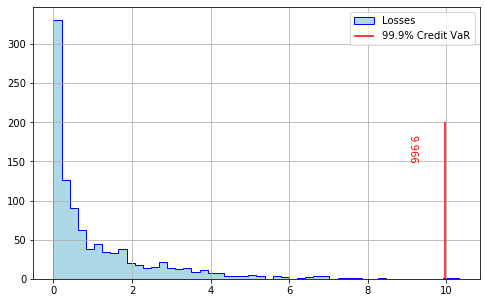
\includegraphics{figures/cr_var_ex}
\end{Answer}






%\clearpage
%\chapter{Machine Learning}\label{ex-lesson-15}

\begin{Exercise}
In order to see how different parameter choices affect the training
(both looking at a plot like the one before and the the \(MSE\)) try to:

\begin{itemize}
\tightlist
\item
  reduce the number of points used in the training (change the step from
  0.1 to 1 or to 0.01 in \(\tt{x = arange(-50, 51, 0.1))}\), expect
  worse results with less points;
\item
  change the number of nodes per layer;
\item
  change the activation function from `sigmoid' to `relu';
\item
  change the number of epochs, this is the number of times the neural
  network will process the sample data to improve the training; setting
  verbose to 1 will show the progress with an estimate of the goodness
  of the training after each epoch; expect worse training with less
  epoch.
\end{itemize}
\end{Exercise}
\begin{Answer}
\end{Answer}

\begin{Exercise}
To see how well our NN behaves with different kind of digits we will try
to check how it works with my calligraphy (as homework try to repeat the
exercise using your own digit following the instructions given below).

\begin{itemize}
\tightlist
\item
  Open \texttt{paint} and create a 280x280 white square
\item
  Change brush type and set the maximum size
\item
  With the mouse draw a digit
\item
  Finally save the file (e.g.~five.png)
\end{itemize}

Before passing the image to the NN it has to be resized and this is done
with an ad-hoc function (\texttt{transform\_image}) which is in the
\texttt{digit\_converter.py} module.
\end{Exercise}
\begin{Answer}
\end{Answer}

\begin{Exercise}
Taking as example the pricing NN trained on call, try to price put
options.
\end{Exercise}
\begin{Answer}
\end{Answer}

%\clearpage

\end{document}
